\documentclass[b4paper,12pt]{book}
   
\usepackage{amsfonts}
\usepackage[serbian]{babel}
 

\usepackage[utf8]{inputenc}
\usepackage{amsmath}
\usepackage{graphicx}
\usepackage{minted}
\usepackage{fixme}
\usepackage{theorem}
\usepackage{algorithm} 
\usepackage{algpseudocode}
\usepackage[table]{xcolor}

\newtheorem{theorem}{Teorema}[chapter]
\newtheorem{definition}{Definicija}[chapter]
%\newtheorem{example}{Primjer}[chapter]{\begin{trivlist}
%		\item[\hskip \labelsep {\bfseries #1}]\end{trivlist}}
\newtheorem{example}{Primjer}[chapter]

\newenvironment{proof}[1][Dokaz]{\begin{trivlist}
		\item[\hskip \labelsep {\bfseries #1}]}{\end{trivlist}}
%\newenvironment{theorem}[1][Teorema]{\begin{trivlist}
%			\item[\hskip \labelsep {\bfseries #1}]}{\end{trivlist}}
 
%\newenvironment{example}[1][Primjer]{\begin{trivlist}
%		\item[\hskip \labelsep {\bfseries #1}]}{\end{trivlist}}
\newenvironment{remark}[1][Remark]{\begin{trivlist}
		\item[\hskip \labelsep {\bfseries #1}]}{\end{trivlist}}
	
\newenvironment{solution}[1][\emph{Rješenje}.]{\begin{trivlist}
			\item[\hskip \labelsep {\bfseries #1}]}{\end{trivlist}}
		
		
		\makeatletter
		\renewcommand{\ALG@name}{Algoritam}
		\makeatother
 
		
		
\begin{document}

\author{Marko Đukanović}
\title{Osnovne algoritamske paradigme kroz programski jezik Pajton}
\date{Januar 2024}

%\frontmatter
 
\maketitle
 
\tableofcontents
 \clearpage
 \setcounter{page}{1}
%\mainmatter

\chapter*{Predgovor}

Ova skripta je napisana za predmet Proceduralno programiranje, koji se obrađuje na prvoj godini Studijskog programa Matematike i informatike -- smjer Informatika na Prirodno-matematičkom fakultetu, Univerziteta u Banjoj Luci. Skipta se sastoji od četiri dijela. Prvi dio obrađuje osnovne pojmove poput pojma programa, algoritma, modela izraču\-navanja, ali bez ulaženja u širinu i sitne detalje, koji se po planu izučavaju na višim godinama iz kurseva Algoritmike. Drugi dio je vezan za osnove programskog jezika Pajton, prvo se obrađuju  osnovni tipovi podatka, složeni tipovi podataka, bitni ugrađeni moduli, pa sve do pisanja korisničkih modula i njihovog postavljanja na zvanični repozitorij \texttt{PyPI}. Treći dio se odnosi na konceptualizaciju osnovnih algoritamskih paradigmi poput paradigme brutalne sile, podijeli pa zavladaj, pohlepnih algoritama, dinamičkog programiranja, te njihovih primjena na rješavanje raznih tipova problema. Četvri dio je vezan za probleme iz aritmetike i njihovo efikasno rješavanje pomoću izloženih algoritamskih paradigmi. 

 Na kraju svake glave se mogu naći zadaci za utvrđivanje materije. Ukupno je više od 40 zadataka dato u ovoj knjizi za utrđivanje naučenih modula, uz oko 30ak riješenih gdje je za većinu njih data kompletna implementacija u Pajtonu uz prateće detalje vezano za korake dizajniranja samih algoritama. 
 
 
 Ovaj udžbenik u nastajanju može služiti studentima nižih godina studija orijenitisanih ka matematici ili informatici ili pak tehničkim naukama u svrhu dograđivanja znanja iz algoritmike (računanja kompleksnosti algoritama, struktura podataka), osnovnih algoritamskih paradigmi te osnova programskog jezika Pajton. Štaviše, mogu ga koristiti i talentovani učenici srednjih škola koji se pripremaju za takmičenja iz informatike. Naime, implementacije problema koje su date u ovoj knjizi se vrlo lako mogu ``prepjevati'' u druge (mnogo brže) jezike nižeg nivoa kao što su C ili C++. Napomenimo da ideja korišćenja jezika Pajton primarno nije bilo da se empirijski osjeti brzina izvršavanja samih algoritama već da se uz pomoć relativno jednostavne i intuitivne implementacije, za što je Pajton neprikosnoven, pokaže primjena raznih algoritamskih paradigmi na rješavanje problema iz akademskog ali i realnog domena.

\chapter{Osnove teorije algoritama}
  U ovoj sekciji uvodimo pojam računskog problema sa fokusom na računarske nauke. Potom uvodimo i pojam algoritma, navodimo neke vrste algoritama te računarskog problema preko uvedenog teorijskog modela računara. Nakon toga se uvode pojmovi složenosti algoritma. Na kraju izlažemo pojam valjanosti algoritma preko metoda invarijantne petlje.  
   
\section{Računski problem}
%https://www.cs.stanford.edu/~trevisan/cs254-10/lecture02.pdf ==> dijelom pratimo:

\textit{Računski problem} (eng. computational problem) u računarskim naukama se jednostavno i slobodno može definisati kao zadatak koji je potrebno riješiti uz pomoć računara. 

Formalna definicija ovog pojma zahtjeva uvođenje mnogih kompleksnih pojmova poput definicije jezika.  U računskom problemu, dat nam je ulaz za koji, bez gubitka opštosti, pretpostavljamo da je kodiran  binarno kao niz iz skupa binarnih nizova proizvoljne dužine $L=\{0, 1\}^*$, a  izlaz je 
rješenje koje zadovoljava neko svojstvo: računski problem  opisujemo  pomoću svojstava koje izlaz mora zadovoljiti s obzirom na (svaki validan) zadani ulaz. Ulaz se često naziva \textit{instanca} problema, dok je izlaz \textit{rješenje} problema s obzirom na ulaz. Primjer računskog programa u računarskim naukama je sortiranje numeričkih nizova. Kao ulaz dat je niz brojeva dužine $n$. Kao izlaz problema sortiranja dobijamo uređen niz (po nekom zadanom kriterijumu sortiranja). Međutim, ne moraju samo numerički nizovi da se sortiraju, već uopšteno, bilo koji objekti nad kojima možemo definisati relaciju totalnog uređenja. Zbog toga ima smisla govoriti o rješavanju računskog problema kao 
 uparivanju ulazno-izlaznih parametara. Ulazni i izlazni parametri mogu se predstaviti nekim matematičkim objektima kao što su brojevi, skupovi, nizovi itd. Ulazni dio problema tada nazivamo \textit{generička instanca} problema, dok izlazni nazivamo  \textit{generiško rješenje} generičke instance problema.  { \begin{color}{red}  Defiicija grafa prije svega? \end{color} }
 
 Postoji nekoliko tipova problema u računarskim naukama; ovdje izdvojimo četiri često prisutna u literaturi: problemi odlučivanja, problemi pretraživanja, problemi optimizacije i problemi prebrojavanja. 
 
 U problemu \textit{odlučivanja}, s obzirom na ulaz $x \in \{0, 1\}^*$, traži se izlaz DA/NE (\emph{True}/\emph{False}). Dakle, u problemu odlučivanja se traži da provjerimo da li instanca problema zadovoljava određeno svojstvo ili ne. Primjer problema odlučivanja je problem \textit{3--bojenja} (3--COL):
 U ulazu problema imamo neusmjereni graf. Potrebno je odrediti da li postoji dodjela   ``boje''  iz skupa $\{1, 2, 3\}$ svakom čvoru grafa tako da niti jedan susjedni čvor nemaju istu dodjeljenu boju.
 
~ Prikladan način za specificiranje problema odlučivanja je detektovanje skupa $L \subseteq \{0, 1\}^*$ ulaza za koje je odgovor DA. Podskup skupa $\{0, 1\}^*$ se takođe naziva jezikom, tako da, uz prethodnu konvenciju, svaki problem odlučivanja može biti specificiran pomoću jezika (a svaki jezik specificira problem odlučivanja). Na primjer, ako sa   3--COL imenujemo podskup skupa $\{0, 1\}^*$ koji sadrži (opise) 3-obojive grafove, tada 3--COL predstavlja jezik koji specificira problem 3-bojenja. %Od sada ćemo govoriti o problemima odlučivanja i jezicima naizmjenično.

U problemu pretraživanja, obzirom na ulaz $x \in \{0, 1\}^*$, potrebno je izračunati neki odgovor
$y \in  \{0, 1\}^*$ koji je u nekom odnosu sa $x$, ako takav  postoji. Dakle, problem pretraživanja je
definisan relacijom $R \subseteq \{0, 1\}^* \times \{0, 1\}^*$, gdje $(x, y) \in R$ ako i samo ako je $y$ dopustiv odgovor  za dati $x$. 

Razmotrimo problem pretraživanja  u vezi sa problemom 3--COL. Dat je
neusmjereni graf $G = (V, E)$, potrebno je pronaći, ukoliko postoji, bojanje $c \colon V \rightarrow \{1, 2, 3\}$
čvorova, tako da za svaki $(u, v) \in V$ vrijedi $c(u) \neq c(v)$. Ovako definisan problem je sada drugačiji (i zahtjevniji) od verzije odlučivanja, jer  od nas se traži  više od toga  --  pored
utvrđivanja postoji li takav $c$, traži se da ga konstruišemo, pod uslovom da postoji.
Formalno, problem 3-bojenja specificiran je relacijom $R_{3-COL}$ koja sadrži sve
parovi $(G, c)$ gdje je $G$ predstavlja 3-obojljivi graf, a $c$ je valjano 3-bojanje grafa $G$.

Problemi optimizacije predstavljaju matematičke probleme koji uključuju pronalazak najboljeg rješenja iz skupa mogućih rješenja. Cilj je maksimizovati / minimizovati   ciljnu funkciju, u odnosu na skup  ograničenja dati definicijom problema. Drugim riječima, cilj je pronaći optimalnu vrijednost određene varijable ili skupa varijabli unutar zadanog skupa ograničenja. Primjer problema optimizacije je klasični ``problem trgovačkog putnika''. U ovom problemu, osoba mora posjetiti skup gradova i vratiti se u   početni grad, sa ciljem da minimizuje ukupnu pređenu udaljenost. Problem se sastoji u pronalasku optimalne rute kojom osoba može posjetiti sve gradove (tačno jednom) uz minimaliziranje ukupne pređene udaljenosti.

Pod problemima prebrojavanja podrazumijevamo matematičke probleme koji uključuju prebrojavanje načina na koje se određeni događaj može dogoditi. Ovi problemi variraju od relativno jednostavnih zadataka kao što je prebrojavanje ljudi u prostoriji do mnogo složenijih scenarija kao što je prebrojavanje    mogućih kombinacija slova u riječi. Pretpostavimo da imamo četiri košulje različitih boja i troje pantalona različitih boja. Na koliko različitih načina se osoba može obući, ako nosimo jednu košulju i jedne hlače?  Za rješavanje ovog problema možemo upotrijebiti princip množenja, koje kaže da ako imamo $ n$ izbora za prvi zadatak i $m$ izbora za drugi zadatak, tada je ukupan broj različitih oblačenja koji se može izvesti jednak  $n \times m$.

Za kraj ovog poglavlja, formalno definišimo računski problem.

\begin{definition}
	Računski problem je funkcija $f \colon \mathbb{N}^* \rightarrow 2^{\mathbb{N}^*}$. $f (x)$ predstavlja skup tačnih odgovora  za ulaz $x$.
\end{definition} 
 
\section{Računarski program i pojam algoritma}
%https://stanford-cs161.github.io/winter2023/lectures/ ==> pratimo lekcije 

Računarski program je (konačan) niz instrukcija napisanih u nekom programskom jeziku koje računar  može da izvrši. Ove instrukcije govore računaru šta da radi i kako da to uradi u eksplicitno definisanom nizu.

Računarski programi mogu biti dizajnirani za obavljanje specifičnih zadataka ili funkcija,  npr. obrada teksta, analiza podataka,  ili pregledavanje veba.  Razvijaju se za različite platforme i operativne sisteme, uključujući desktop računare, mobilne uređaje, ugrađene sisteme itd.  Kompjuterski programi se mogu kreirati korišćenjem raznih programskih jezika, kao što su Pajton, Java, C++  i mnogi drugi. Kada je program napisan, potrebno ga je kompajlirati ili interpretirati u mašinski k\^od koji je razumljiv procesoru računara. Rezultirajući izvršni k\^od korisnici mogu pokrenuti kako bi izvršili željene zadatke ili funkcije.
%https://www.geeksforgeeks.org/introduction-to-algorithms/

Algoritam predstavlja  korak-po-korak postupak za rješavanje problema ili postizanja određenog   cilja. U informatici, algoritmi se su predstavljeni konačnim  niza instrukcija koje kompjuterski program slijedi da bi riješio određeni problem ili izvršio određeni zadatak. Algoritam najčešće počinje sa inicijalnim ulazom, koji zatim nizom logičkih koraka ili operacija dovodi do očekivanog izlaza ili rezultata.  Analogija algoritma u stvarnom svijetu se može predstaviti primjerom kuhanja po receptu. Da biste skuhali po receptu, neophodno je čitati uputstva i korake te ih izvršavati jedno po jedno, u datom redoslijedu. Dobijeni (očekivani) rezultat je jelo koje je kuhano.  

 Primjeri dobro poznatih algoritama uključuju algoritme za sortiranje koji se koriste za uređivanje podataka u odnosu na relaciju  uređenja, algoritme pretraživanja koji služe za pronalaženje određenih informacija na velikom skupu podataka, zatim algoritme dešifrovanja i druge.  %koji se koriste za zaštitu osjetljivih informacija od neovlaštenog pristupa.

Algoritmi su korisni iz više razloga:
\begin{itemize}
	\item   Neophodni su za efikasno i efektivno rješavanje složenih problema.
	
	\item  Pomažu u automatizaciji procesa -- čine ih pouzdanijim, bržim i lakšim za izvođenje.
	
	\item  Omogućavaju računarima da izvršavaju zadatke koje bi ljudima bilo teško ili nemoguće izvršiti ručno.
	
	%\item korisi u raznim oblastima kao što su matematika, računarstvo, inženjering, finansije itd. za optimizaciju procesa, analizu podataka, predviđanje i pružanje rješenja za probleme.
\end{itemize}
Ne određuje svaki niz instrukcija jedan algoritam. Da bi neke instrukcije činile algoritam, sljedeće karakteristike treba da budu ispoštovane:

\begin{itemize}
    \item    \textit{Dobro definisani ulazi}: Ako algoritam zahtjeva podatke u ulazu, podaci bi trebali biti dobro definisani. 
    \item \textit{Dobro definisani rezultati}: Algoritam mora jasno definisati koji će se rezultat dobiti (kao izlaz) u zavisnosti od svakog ulaza. %Trebalo bi da vrati najmanje jedan izlaz.
    \item    \textit{Konačnost}: Algoritam mora biti konačan, tj. trebao bi se prekinuti nakon konačnog vremena za sve testne slučajeve. Beskonačne petlje ili rekurzivne funkcije bez baznih uslova ne posjeduju svojstvo konačnosti; o ovome ćemo govoriti u nastavku.  
    \item  \textit{Dopustivost}: Algoritam mora biti generički i praktičan, u smislu da se može izvršiti u okviru dostupnih resursa.  %Ne smije sadržavati neku buduću tehnologiju ili bilo šta drugo.
      \item \textit{Nezavisnost od jezika:} Algoritam koji je dizajniran mora biti nezavisan o jeziku u kojem se implementira; dakle, izlaz invarijantan od jezika imlementacije.
      \item   \textit{Definisanost}: Sve instrukcije u algoritmu moraju biti nedvosmislene, precizne i lake za interpretaciju. Pozivanjem  bilo koje  instrukcije algoritma,   jasno se može razumjeti šta ona radi. Svaki osnovni operator u instrukciji mora biti definisan bez   nejasnoća.  
      %\item \textit{Učinkovitost}: Algoritam se mora razviti korištenjem vrlo osnovnih, jednostavnih i izvodljivih operacija tako da se može rekonstruisati (čak i na papiru).  %koristeći samo papir i olovku.
\end{itemize}
Koncizno rečeno, svaki algoritam posjeduje sljedeće karakteristike:  
\begin{itemize}
	\item Završava se nakon određenog vremena.
    \item Vraća barem jedan izlaz.
    \item Ima ulaz domenzije nula ili više.
    \item Posjeduje determinizam, tj. svaki put daje isti izlaz za isti ulazni slučaj.
    \item Svaki korak u algoritmu je efikasan, tj. svaki korak bi trebao obaviti određeni posao.
\end{itemize}

\textit{Veličina ulaza} algoritma je defisana kao ukupan broj elemenata prisutnih u ulazu. Za dva problema, veličina ulaza $n$ može biti okarakterisana na drugačiji način.  Npr.  u problemu sortiranja to  je ukupan broj stavki za sortiranje, dok je to  u problemima sa grafovima  ukupan broj čvorova i grana, a  u numeričkim problemima je to ukupan broj bitova potrebnih za predstavljanje broja. 

 %https://www.geeksforgeeks.org/introduction-to-algorithms/ ==> Types of algorithms...
 \subsection{Vrste algoritama}
Na raspolaganju je nekoliko tipova (paradigmi) algoritama. Neke važnije paradigme nabrajamo u nastavku. 
\begin{enumerate}
	\item Algoritmi \textit{brutalne sile} (eng. \textit{brute force}): jedan od najjednostavnijih pristupa rješaanja problema. Ujedno je i prvi pristup koji se konstruiše za  rješavanje problema jer je ideja rješenja u pozadini često vrlo naivna te se razmatraju svi mogući slučajevi koji  potencijalno mogu predstaviti rješenje problema.
	\item \textit{Rekurzivni algoritmi}: Ovi algoritmi su zasnovani na rekurziji. U ovom slučaju, problem se dijeli na nekoliko podproblema te  se ista funkcija poziva iznova za rješavanje tih podproblemima, dok god se ne dođe do nekih trivijano rješivih slučajeva.
	\item \textit{Algoritam vraćanja unazad}: Ovo je algoritamska tehnika rekurzivnog rješavanja problema koja pokušava postepeno izgraditi rješenje, dio po dio, isključujući momentalno ona rješenja koja ne uspijevaju zadovoljiti ograničenja problema. 
	\item  \textit{Algoritmi pretraživanja}:  Oi algoritmi se koriste za pretraživanje elemenata ili grupa elemenata iz određene strukture podataka. Mogu biti različitih tipova na osnovu njihovog pristupa ili strukture podataka u kojoj se element nalazi.
	\item \textit{Algoritmi sortiranja}: Sortiranje je uređivnanje grupe podataka  shodno nekom kriterijumu. Algoritmi koji pomažu u obavljanju ove funkcije nazivaju se algoritmi sortiranja. %Sortiranje grupa podataka na rastući ili opadajući način.
	\item \textit{Algoritam podijeli i vladaj}: Ovaj algoritam razbija problem na podpro\-bleme, rješava podprobleme i spaja njihova rješenja kako bi se dobilo konačno rješenje. Sastoji se od sljedeće tri procedure:
    podijeli, riješi, kombinuj. Ovo je, inače, algoritamska paradigma koja se koristi u rješavanju raznih tipova problema poput sortiranja.
  
    \item \textit{Pohlepni algoritmi}: U ovom tipu algoritma rješenje se gradi konstruktivno, komponentu po komponentu.   Komopnenta koja daje najveću korist pri dodavanju na trenutno rješenje, biće i uzeta kao komponenta koja  proširuje trenutno  rješenje. Odabir  narednog rješenja u nizu donosi se na osnovu nekog (pohlepnog) kriteijuma.
    \item \textit{Dinamičko programiranje}: Ovaj tip algoritma koristi koncept korištenja već pronađenog rješenja (koje se čuva u memoriji) kako bi se izbjeglo ponavljanje izračunavanja istog dijela problema. Ova paradigma dijeli problem na manje podprobleme, koji se preklapaju, a potom ih rekurzivno rješava.
\end{enumerate}
   
   Većina ovih tipova algoritama predstavljaju generičke sheme (paradigme) koje se mogu primijeniti na  rješavanje većeg opsega različitih problema. Tu pripadaju algoritmi brutalne sile, rekurzivni algoritmi, podijeli i zavladaj, algoritam vraćanja unazad, pohlepni algoritmi, dinamičko programiranje isl. U glavi 3 biće detaljno obrađene  neke od pomenutih paradigmi. \\
  
Dizajniranje efikasnog algoritma je obično dugotrajan proces koji nije direktan, te zahtijeva veliko domensko znanje o problemu te domišljatost onoga koji rješava vezano za način rješavanja samog  problema.  Međutim, postoje neka pravila kojima se vodimo kada konstruišemo algoritam, kao što su korištenje paradigmi za koje znamo da su dovoljno efikasne u rješavaju određenog tipa problema. 
 \\ 
 
 U nastavku govorimo malo o istorijskoj pozadini nastanka riječi \textit{algoritam}. Riječ ``Algoritam'' je iskrivljena transliteracija imena ``al-Khwarizmi''. Al-Khwarizmi bio je persijski matematičar iz IX veka, rođen na prostorima današnjeg Uzbekistana, studirao i radio u Bagdadu za vrijeme Abasidskog kalifata; oko 820. godine nove ere imenovan je za
  šefa biblioteke ``Kuće mudrosti'' u Bagdadu. Napisao je nekoliko
 uticajnih knjiga, uključujući i jednu sa naslovom ``O kalkulaciji sa hinduistanskim brojevima'', koja opisuje kako se izvodi aritmetika koristeći arapske brojeve (aka arapsko-hindu, a kraće hinduistički brojevi). Originalni rukopis je izgubljen, ali latinski prevod iz 
 1100. godine uveo je ovaj brojevni sistem u Evropu te se smatra odgovornim  za današnje korišćenje  arapskih brojeva.   Stara francuska riječ \textit{algorisme} značila je
 ``arapski numerički sistem'', a tek kasnije je postao opšti recept za rješavanje računskih problema.

\section{Teorijski RAM model}

Pri razvoju algoritama, postavljaju se nekoliko ključnih pitanja: 
\begin{enumerate}
	\item Da li je naš algoritam efikasan? 
	\item Da li je jedan algoritam brži od drugog? 
	\item Koliko je najgore očekivano vrijeme izvršavanja algoritma za ulaze velikih dimenzija? 
\end{enumerate}
 

Odgovor na ova pitanja nije trivijalan, i zahtjeva uvođenje stroge matematičke notacije i modela izračunljivosti. 

Najprije uvedimo pojam \textit{mašine sa slučajnim pristupom} (eng. \textit{random access machine}), teorijskog modela računara.  Mašina sa slučajnim pristupom može da izvršava instrukcije i manipuliše podacima. Ova mašina pretpostavlja da je memorija  %koja se može zamisliti kao beskonačna traka,  
podijeljena na diskretne ćelije, od kojih se svakoj može pristupiti i direktno modifikovati njen sadržaj, te da mašina izvršava instrukcije na sekvencijalni način (ne postoji paralelizam).

Mašina sa slučajnim pristupom predstavlja varijaciju RAM modela koji uključuje randomizaciju u svojim operacijama. Gledajući fizički RAM model, redoslijed instrukcija je fiksan, ali u RAM-u se neke operacije mogu nasumično rasporediti. Npr. RAM može imati ``slučajnu''  instrukciju koja nasumično odabira ćeliju u memoriji i izvodi odgovarajuću operaciju u odabranoj ćeliji.

Ova mašina predstavlja model (apstrakciju) koja se koristi u analizi algoritama i njihove složenosti jer omogućava \textit{precizno} izračunavanje broja instrukcija potrebnih za obavljanje određenog zadatka. Ovaj model pretpostavlja da su vremena pristupa memoriji konstantna, što nije tačno na realnim računarima. U praksi, pristup memoriji može uzimati različito vrijeme ovisno o faktorima kao što su keširanje, pristup disku i kašnjenje mreže.

%http://people.seas.harvard.edu/~cs125/fall14/lec6.pdf ==> follow
\subsection{Instrukcije u RAM modelu}
Krenimo sa formalizovanjem teorijskog modela koji 
se standardno koristi za analizu algoritma.  Posmatrajući viši nivo,   karakteristike modela su sljedeće:

\begin{itemize}
	\item Glavna memorija je niz $M = (M[0], \ldots, M[S-1])$  $w$-bitnih riječi, koje se takođe mogu prikazati kao brojevi u intervalu
 $\{0,\ldots , 2^w - 1\}$.
 	\item Niz $R = (R[0], \ldots , R[r - 1])$,  gdje je $r$ broj registara, koji su takođe $w$-bitne riječi. Registri se koriste za privremeno pohranjivanje podataka tokom izvođenja programa, te za pohranjivanje adresa za dohvaćanje podataka iz RAM-a.  %, kao i za čuvanje privremenih rezultata izračunavanja. 
 	
 	\item Algoritmima je dozvoljen samo direktan pristup registrima. Preostalim memorijskim lokacijama može se pristupiti samo
 	indirektnim adresiranjem -- intepretirajući riječi (u registru) kao pokazivač na drugu memorijsku lokaciju. Dakle, zahtjevamo
 	$S \leq  2^w$.
 	\item Program je konačan niz instrukcija.
 	\item Skup instrukcija se sastoji od osnovnih aritmetičkih i bitskih operacija nad riječima (u registrima), kondicionalima
 	(\texttt{if}--\texttt{else}), \texttt{goto}, kopiranja riječi između registara i glavne memorije, zaustavljanja.
 	\item Dopuštamo \texttt{\textit{malloc}} operaciju, tj. dodavanje dodatne memorijske ćelije, povećavajući $S$ eksplicitno (i $w$ ako je potrebno da osiguramo $S \leq 2^w$).
 	\item Početna konfiguracija memorije je sljedeća:
 	($i$) Ulaz veličine $n$ smješten je u glavne memorijske lokacije $(M[0],\ldots , M[n - 1])$; ($ii$) Veličina riječi postavljena je na $w = \lfloor \log_2 \max\{n + 1, k + 1\} \rfloor $, gdje je $k$ gornja granica za brojeve koji se
 	pojavljuju ili u ulazu ili kao konstanta u programu; ($iii$) Registar 0 se inicijalizira sa $w$, a registar 1 sa $n$.
 \end{itemize}

Formalno, dopuštene se sljedeće instrukcije (u RAM modelu) za indekse $i, j, k, m \in \mathbb{N} $:

%\begin{figure}[H]
%	\centering
%	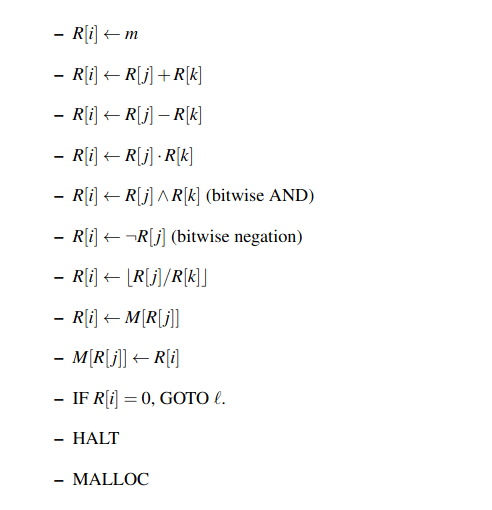
\includegraphics[width=300pt,height=280pt]{slike/instructions_ram.png}
%
%	\caption{Pregled instrukcija u RAM modelu.}	\label{fig: ram_instructions}
%\end{figure}

\begin{itemize}
	\item $R[i] \gets m$ (dodjela)
	\item $R[i] \gets R[j] \pm R[k]$
	\item $R[i] \gets R[j] \cdot/ R[k] $
	\item $R[i] \gets R[j] \/ R[k] $
	\item $R[i] \gets R[j] \wedge R[k]$
	\item $R[i] \gets \neq R[j] $ (bitovska negacija)
	\item $R[i] \gets M[R[j]]$
	\item $M[R[j]] \gets R[i]$
	\item IF $R[i] = 0$, GOTO $l$
	\item HALT
	\item MALLOC (inicijalizacija dodatne memorije)
	\item $\vdots$
\end{itemize}

\begin{definition}
   ${w}$-RAM program je bilo koji konačan niz instrukcija $P = (P_1, P_2,\ldots, P_q)$ gore navedenog tipa. Broj $r$ registara je implicitno definisan kao  najveći indeks direktne memorijske adrese (među indeksima $i, j, k$ skupa instrukcija) koji se javljaju u programu.
\end{definition}

\subsection{Formalizacija programa na RAM-u}

Pojam konfiguracije ima za cilj da obuhvati cjelokupno stanje računanja u određenom trenutku --  sve što je neophodno za određivanje budućeg ponašanja.
\begin{definition}
Konfiguracija  \emph{w}--RAM programa $P$ je torka $K = (l, S, w, R, M)$, gdje je $l \in  \{1, \ldots, q + 1\}$ 
programski brojač, $S \in  \mathbb{N}$ je korišteni prostor, $w \in  \mathbb{N}$ je veličina riječi, $R = (R[0], \ldots , R[r - 1]) \in  \{0, \ldots , 2^w - 1\}^r$ je
niz registara, i $M = (M[0], \ldots, M[|S| - 1]) \in  \{0, \ldots, 2^w - 1\}^{|S|}$ je memorijski niz.
\end{definition}
%%https://medium.com/@_SD10_/the-ram-model-of-computation-and-big-o-notation-a1b3cc50ec2c
\begin{definition}
 Za konfiguraciju $K = (l, S, w, R, M)$ \textit{w}-RAM programa $(P_1, \ldots, P_q)$ definišemo sljedeću konfiguraciju $K' = (l', S', w', R', M')$, u zapisu $K$ $\Rightarrow_P K'$, na sljedeći način:
 
 \begin{itemize}
 	\item Ako je $P_l$ = ``IF $R[i] = 0$, GOTO $m$'' za neke $i < r$ i $m \in  \{1, \ldots , q\}$, onda  $K' = (l', S, w, R, M)$ gdje je  $l'= m$ ako je $R[i] = 0$, a $l' = l + 1$ inače. 
 	\item Ako je $P_l$ = ``$R[i] \leftarrow  m$'' za $i < r$, onda $K' = (l  + 1, S, w, R', M)$ gdje  $R'[i] = m$ \emph{mod} $2^w$ i $R'[ j] = R[ j]$ za sve $j \neq i$. 
 	\item Ako je $P_l$ = ``$R[i] \leftarrow R[ j] + R[k]$'' za neki $i, j, k < r$, onda  $K' = (l+1, S, w, R', M)$   gdje je $R'[i] = (R[ j]+R[k])$ \textit{mod} $2^w$
 	i $R'[j] = R[j]$ za sve $j \neq i$.
 	\item Ako je $P_l$ = ``$M[R[ j]] \leftarrow R[i]$'' za $i, j < r$ i $R[ j] < S$, onda $K' = (l+ 1, S, w, R, M')$ gdje je $M'[R[ j]] = R[i]$ i
 	$M'[k] = M[k]$ za sve  $k \neq  R[ j]$.
 	\item Ako je $P_l$ = ``MALLOC'', onda je $K' = (l+ 1, S + 1, w', R, M')$, gdje je $w' = \max\{w, \lceil log_2(S + 1) \rceil \}$, $M'[S] = 0$ i
 	$M'[i] = M[i]$ za $i = 0, \ldots , S-1$.
 	\item Ako je $P_l$ = ``HALT ili  $l = q + 1$'', onda je $K' = (q + 1, S, w, R, M)$.
 \end{itemize}
 
 
\end{definition}

Napomenimo da smo prethodno naveli   samo neke od instrukcija, dok se ostale definišu slično. \\


Definišimo sada formalno pojam računarskog problema shodno prethodno definisanom pojmu RAM modela. 
\begin{definition}
	 RAM program $P = (P_1, \ldots, P_q)$ sa $r \geq 2$ registara rješava problem $f \colon \mathbb{N}^* \rightarrow 2^{\mathbb{N}^* } $
	ako za svaki ulaz $x = (x_1,\ldots, x_n) \in \mathbb{N}^* $ i $k \geq \max\{x_1,\ldots, x_n, m\}$ gdje je $m$ najveća konstanta koja se pojavljuje u $P$, postoji niz konfiguracija $K_0,\ldots,K_t$ tako da:
	\begin{itemize}
		\item $K_0 = (1, n, w, R, M)$ gdje je $w = \lceil \log_2(\max\{n, k +1\})\rceil$, $R[0] = n$, $R[1] = k$, $R[2] = R[3] = \cdots =  R[r-1] = 0$, $M[0] = x_1,
		M[1] = x_2, \ldots , M[n - 1] = x_n$,
		\item $K_{i-1} \Rightarrow_P K_i $ za sve $i = 1, \ldots ,t$,
		\item $K_t = (q+1, S, w, R, M)$ gdje je $(M[1], M[2], \ldots , M[R[0] - 1]) \in  f (x)$. 
	\end{itemize}
\end{definition}

\textit{Komentar}.  Ključne tačke u vezi teorijskog RAM modela su:
\begin{itemize}
	\item  \textit{Ujednačenost}: zahtijevamo da postoji konačan program koji bi trebao raditi za proizvoljne ulaze neograničene veličine
(kad $n, k \rightarrow \infty$).
    \item Računanje se odvija nizom “baznih” operacija.
    \item Ne namećemo a priori ograničenje za vrijeme (broj koraka) ili prostor   (memorija). Ove resurse 
      želimo minimizirati, ali i dalje teorijski RAM model  smatra  algoritmom čak i ako on koristi ogromne količine vremena i prostora, što se, vidjećemo, razlikuje od praktičnog aspekta algoritama. 
\end{itemize}

Pri računanju broja instrukcija izvršavanja programa $P$, u obzir uzimamo sljedeće operacije: aritmetičke i bitske operacije (+, -, *, /, \&, $\mid,\ldots $), logičke ($\wedge$,$\vee$, $\Rightarrow$, $\Leftrightarrow$), operacija dodjele, te ulazno/izlazne operacije. Ove operacije nazivamo \textit{jediničnim instrukcijama}.  Pretpostavka je da se sve jednične instrukcija izvršavaju u jediničnom vremenu.  Vremenska složenost programa se upravo mjeri na osnovu ukupnog broja jediničnih instrukcija, o čemu ćemo više reći u narednoj sekciji. 

\section{Pojam složenosti algoritma}

Napomenimo da je jediničnim modelom složenosti definisan (teorijski) RAM model gdje se svaka operacija izvršava u jediničnom vremenu.  Bez obzira što operacije sabiranja i množenja nemaju isto vrijeme izvođenja na stvarnom računaru, to ne umanjuje značaj teorijskog RAM modela, što ćemo prikazati u nastavku.   

Definišimo sada vremensku složenost izvršavanja programa $P$ na RAM modelu.

\begin{definition}
	Vrijeme rada $P$ za ulaz  $x \in \mathbb{N}^*$ je broj $t$ koraka prije nego $P$ dostigne zaustavnu
	konfiguracija (operacija ``HALT'') za $x$. Dakle, najmanji $t$ za koji postoji niz $K_0 \Rightarrow_P  K_1 \Rightarrow_P \cdots \Rightarrow_P K_t$ takav da je $K_0$
	početna konfiguracija od $P$ za ulaz $x$, a $K_t$ je konfiguracija zaustavljanja (gdje se programski brojač  ažurira na $q + 1$, a $q$
	označava broj instrukcija u programu $P$).  
	Pogledajmo sljedeći primjer. 
	
\end{definition}
 
%\begin{example} \\
	
\begin{minted}{C}
	algoritam max(a, n)
	  maximum = a[0]
 	  for i in 1 to n-1 do
	      if a[i] > maximum then
                  maximum = a[i]
          return maximum    
\end{minted}

%\end{example}

Izračunajmo tačan broj instrukcija programa konkretnog ulaza $a = [1\ 5\ 2\ 10\ 7]$ i $n = 5$. Imamo: prva linija sadrži jednu instrukciju (dodjela). Unutar petlje (koja se izvršava $n-1$ puta, za koju se dodjeljuje nova  vrijednost iteratoru \texttt{i}, te se potom provjerava da li je ona veća od $n$), broj instrukcija koji je uvjetovan prolazom elementima niza  $\texttt{a}$ je $5, 3, 5$ i $3$, što je ukupno $1+5+3+5+3=17$ izvršenih instrukcija.  U kombinaciji sa instrukcijama za varijable \texttt{i} u \emph{for} petlji, ovaj program izvršava ukupno $17+ 4 \cdot 2 + 1 = 26$ instrukcija.



Vremenska složenost izvršavanja programa se mjeri u odnosu na ukupan broj
jediničnih instrukcija. Tačan broj instrukcija za svaki ulaz u kompleksnim programima je     teško precizno izračunati. Zbog toga uvodimo pojam \textit{najgoreg vremena izvršavanja} programa (eng. \textit{worst-case running time}) koji nam pruža   lakši način računanja broja instrukcija programa, ali opet dovoljno reprezentativan da ukaže na to koliko je algoritam efikasan. 

\begin{definition}
	  Najgore vrijeme izvršavanja programa $P$ je funkcija $T \colon \mathbb{N} \times \mathbb{N} \rightarrow \mathbb{N}$ gdje je $T (n, k)$ maksimalno
	vrijeme rada programa $P$ u odnosu na sve moguće ulaze $x \in  \{0, \ldots , k\}^n$.
\end{definition}

\begin{example} 
	
	Pogledajmo sljedeći program  \\  \vspace{0.3cm} 
\begin{minted}{Python}

algoritam sort(a, n)
  for i in 1  to n-1 do
     for j in 0 to  i-1 do
        if a[i] > a[j] then
           swap (a[i], a[j])
           
           	\end{minted}
\end{example}

Najgori slučaj za ulazne podatke je kada se instrukcije pod \emph{if}--petljom stalno izvršavaju; to je slučaj kada je na ulazu niz \texttt{a} kojem su elementi poredani u obrnutom  poretku u odnosu na traženi poredak. Prema tome \texttt{swap} operacija se tada izvršava u svakoj iteraciji, i ona sadrži 3 instrukcije (dodjela). Unutrašnja petlja se izvršava $i$ puta  za svaki $i=1, \ldots, n-1$.  Tada imamo da je  
$$ \sum_{i=1}^{n-1} \sum_{j=0}^{i-1} 2 \cdot 3 = 6 \sum_{i=1}^{n-1} i = 3 \cdot {(n-1) \cdot n}$$ najveći (najgori) broj instrukcija koji algoritam izvršava za svaki ulaz dužine $n$. 
\\


Za najgore vrijeme izvršavanja  uzimamo najgori slučaj ulaznih podataka određene dimenzije za koji će se izvršiti maksimalan broj instrukcija. Motivacija za računanje najgoreg vremena izvršavanje programa (algoritama) je sljedeća. Najgori slučaj izvršavanja algoritma je obično lakši za detektovanje i izračunavanje nego je to slučaj sa   tačnim brojem koraka (instrukcija) za konkretnu instancu, koji ne govori mnogo o broju instrukcija programa za ulaze drugačijih distribucija. Prepoznavanje najgoreg slučaja za ulazne podatke određene dimenzije za koje program radi najduže nam omogućuje da utvrdimo gornju granicu za broj instrukcija svakog mogućeg izvršenja programa. Ovakvo vrijeme izvršavanja ne  zavisi od konkretne (distribucije) ulazne instance, čime se dobija bolji osjećaj o efikasnosti programa u odnosu na veličinu ulaza.
 
Bez obzira na ovakva pojednostavljenja, i dalje je egzaktno računanje najgoreg vremena izvršavanja težak posao u većini kompleksnih programa. Stoga, u nastavku govorimo o pojmu \textit{asimptotskog} vremena izvršavanja programa.  Gotovo uvijek se broj koraka izvršavanja u algoritmu povećava shodno povećavanju dimenzije ulaza. Prema tome, ima smisla posmatrati ponašanje algoritma na  
ulazima velike dimenzije jer se često programi čiji su ulazi  malih dimenzija ionako efikasno izvršavaju (imaju kratko vrijeme izvršavanja)  nezavisno od algoritamske tehnike rješavanja. U sljedećoj podsekciji, formalno uvedimo pojam $O$--notacije. 
 
 
\subsection{$O$--notacija} 
$O$-notacija   dodatno pojednostavljuje ocjenjivanje broja izvršenih instrukcija  programa, fokusirajući se na ponašanje algoritma na ulazima velikih dimenzija.  Pretpostavimo da imamo sljedeću situaciju o ocjeni najgoreg scenarija izvršavanja dva algoritma (na istom posmatranom problemu): 
\begin{itemize}
	\item $T_1(n) = 2 n^{\frac{3}{2}} + 3n + 10$
	\item $T_2(n) = 4 n \cdot \log n + \lceil \sqrt{n} \rceil + 22 $
\end{itemize}

Upoređivanje ovakvih funkcija zahtjeva analitičku analizu obje funkcije, pri čemu se može utvrditi da je prvi algoritam (koji se izvršava u $T_1$ vremenu u odnosu na ulaz veličine $n$)  brži -- zahtjeva izvođenje manjeg broja instrukcija -- za manje $n$, dok je za veće $n$ očigledno u prednosti algoritam sa vremenom izvršavanja $T_2$ ($n \log n$ dosta sporije raste od funkcije $n^{\frac{3}{2}}$). 

Dakle, cilj je je pojednostaviti računanje izvršenog broja instrukcija, koje se postiže uvođenjem sljedećih konvencija u svrhu ocijenjivanja ponašanja algoritma na instancama velikih dimenzija.
\begin{enumerate}
	\item Konstante uz svaki od termova se ignorišu.
	\item Dominantni termovi se uzimaju, dok se ostali (nedominirajući) ignorišu. Dominantan je onaj term koji najbrže raste sa porastom dimenzije ulaza. Dakle, procjenjuje se asimptotsko ponašanje broja instrukcija u zavisnosti od veličine ulaza programa. 
\end{enumerate}

Za $T_1(n)$  je dominantni term funkcija $n^{\frac{3}{2}}$, dok je to za $T_2(n)$ funkcija $n \cdot \log n$. 
 
 Nadalje pretpostavimo da radimo sa pozitivnim funkcijama, sa pozitivnim vrijednostima argumenata. 

%%https://www.khanacademy.org/computing/computer-science/algorithms/asymptotic-notation/a/big-o-notation

\begin{definition}
Neka su date dvije funkcije $f$ i $g$. Kažemo da $f = O(g)$ akko postoji konstanta $c >0$ tako da $f(n) \leq c \cdot g(n)$ počevši od nekog dovoljno velikog $N$. tj. za $n \geq {N}$. Kažemo da je $g$ (gornja) asimptotska granica za $f$. 
\end{definition}

\begin{figure}[H]
	\centering
	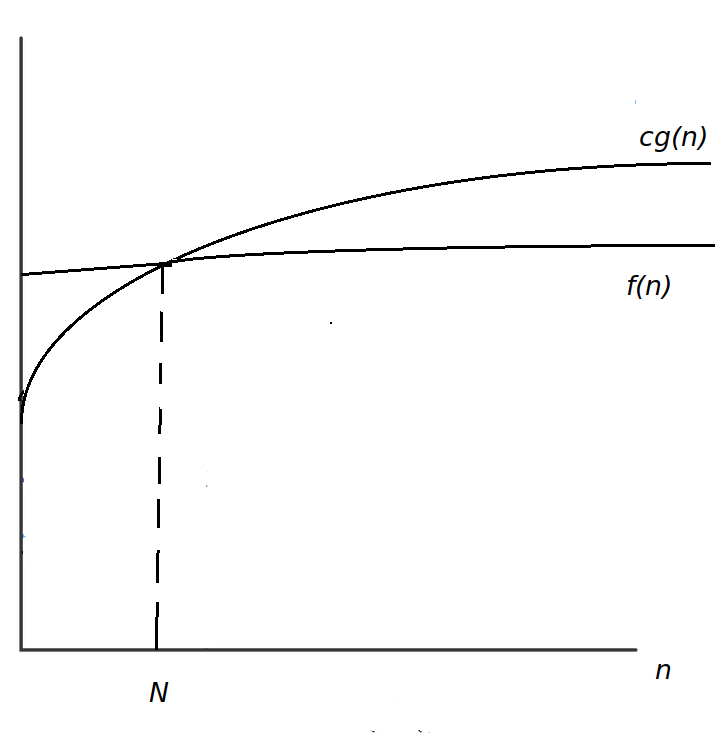
\includegraphics[width=170pt,height=170pt]{slike/O_notation.png}
	\label{fig:O_notation}
	\caption{$O$--notacija: vizuelizacija.}
\end{figure}


%https://afteracademy.com/blog/time-and-space-complexity-analysis-of-algorithm/

\begin{example}
	Jasno je da $T_1 = O(n^2)$, ali i $T_1 = O(n^{\frac{3}{2}})$. Takođe, $T_2 = O(n \log n)$. 
\end{example}

U osnovi, dominirajući term nam govori o asimptotskoj granici čitavog izraza (dobijen računanjem (najgoreg mogućeg) broja instrukcija izvršenog u programu), jer kad je $n$ dovoljno veliko, vrijednost izraza dominantno zavisi od dominirajućeg terma, dok se ostali termi doprinose u ne tako značajnoj mjeri da bi se promijenio zaključak o asimptotskom ponašalju porasta broja instrukacija programa sa porastom dimenzije ulaza. 

$O$--notacija, bez obzira na praktičnost i jednostavnost, dovodi i do određenih  dvosmislenosti. Npr.\  $n^2 + n = O(n^2)$, ali vrijedi i $n^2 + n = O(n^3)$. U svakom slučaju, korisniji zaključak dobijamo uzimajući prvi od ova dva.  Ovo nas dovodi do definisanja $\Theta$--notacije (eng. Big-Theta).

\begin{definition}
Neka su date dvije funkcije $f$ i $g$.  Ako $f = \Theta(g)$, onda postoje konstante $c_1, c_2 >0$ tako da $c_1 g(n) \leq f(n) \leq c_2 g(n)$, počevši od nekog dovoljno velikog $n$. 
\end{definition}

U prevodu, funkcije $f$ i $g$ imaju isto asimptotsko ponašanje (dakle, za velike vrijednosti ulaza $n$), vidjeti Sliku~\ref{fig:theta_notation}. 

\begin{figure}[H]
	\centering
	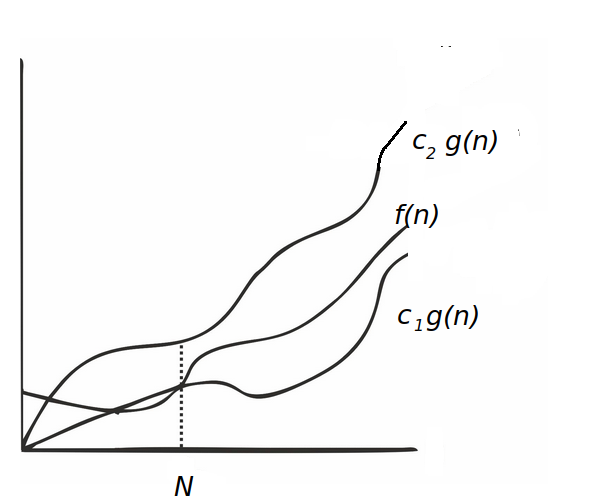
\includegraphics[width=170pt,height=150pt]{slike/theta-notation.png}
 
	\caption{$\Theta$--notacija: vizuelizacija za slučaj $f(n)=\Theta(g(n))$.}	\label{fig:theta_notation}
\end{figure}

\begin{example}
Imamo	$T_1 = \Theta(n^{\frac{3}{2}})$, dok je $T_2 = \Theta(n \log n)$.  
\end{example}

Postoji još nekoliko notacija za složenost algoritama, a to su $\Omega$ i $o$--notacija.

\begin{definition}
 Neka su date dvije funkcije $f$ i $g$. Kažemo da $f = \Omega(g)$ akko postoji konstanta $c >0$ tako da je $f(n) \geq c g(n)$, počevši od nekog dovoljno velikog $n$.  
\end{definition}
$\Omega$-notacija govori o funkcijama za koje je $g$ asimptotska donja granica, budući da ograničava rast vremena rada odozdo za dovoljno velike veličine ulaza.

\begin{example}
  Vrijedi $n^3= \Omega(n^2 + n)$ i $n\log n = \Omega(n)$.
\end{example}

\begin{definition}
	Neka su date dvije funkcije $f$ i $g$. Kažemo da $f = o(g)$ akko za sve $c > 0$ postoji   $N > 0$ takav da je $0 \leq f(n) < cg(n)$ za sve $n \geq N$. 
	
\end{definition}

\noindent \textbf{\textit{Napomena}}. Vrijednost $k$ ne smije zavisiti od $n$, ali može da zavisi od $c$.

Neformalno, ako $f(n) = o(g(n))$, to znači da  $f$ postaje beznačajno mala u odnosu na $g$ kako se $n$ približava beskonačnosti.

\begin{example}
    Vrijedi $n = o(n^2)$, kao i $n = o(n^3)$, ali ne vrijedi $n = o(n)$. 
\end{example}

\subsection{Neka svojstva $O$--notacije}

\begin{theorem} Neka su $f, g$ i $h$ pozitivne funkcije, pozitivnih vrijednosti argumenata.  Vrijede sljedeće tvrdnje:
	\begin{itemize}
		\item 	  $f = O(c \cdot f)$ za svako $c > 0$ (konstantni faktori su irelevantni);
		\item Ako $f = O(g +  h)$ i $h = O(g)$, onda je i $f = O(g)$  (pravilo dominantnog terma);
		\item $O(f + g) = O(f)  + O(g)$ (pravilo zbira);
		\item $O( f \cdot g) = O(f) \cdot O(g)$ (pravilo proizvoda);
        \item $f = O(g)$ i $g = O(h)$ onda
        vrijedi i $f = O(h)$ (pravilo tranzitivnosti). 
	\end{itemize}
 
\end{theorem}

\begin{proof}
	Dokazi tvrdnji se direktno izvode na osnovu definicije $O$--notacije.
\end{proof}

\subsection{Uputstva za procjenu složenosti algoritama}

Prethodna sekcija nam daje na uvid neke od osnovnih notacija za ocjenjivanje složenosti   algoritma, tj. izvršenja broja instrukcija programa koja se obično razmatra u zavisnosti od veličine ulaza. 

 Najčešće funkcije koje se pominju u analizi složenosti izvršavanja algoritama su nabrojane u Tabeli~\ref{tab:slozenosti_funkcije-a}. 
 
 \begin{table}[H]
 	   \caption{Česte klase $O$--složenosti. }  \label{tab:slozenosti_funkcije-a}
 	\centering 
 	\begin{tabular}{l |l} \hline 
 		\textbf{Funkcija}   &  \textbf{Klasa složenosti} \\ \hline
 		1          & konstantna \\
 		$\log n$   & logaritamska \\
 		$n$        &  linearna \\
 		$n \log n$ & super-linearna  \\
 		$n^2$      & kvadratna \\
 		$n^3$      & kubna \\
 		$2^n $     & eksponencijalna \\ 
 		$n!$       & faktorijel \\
 		\hline
  	\end{tabular}

 \end{table}
 Rast nekih funkcija sa porastom ulaza ($n$) je prikazan na Slici~\ref{fig:slozenosti_funkcije-a}
 \begin{figure}[H]
 	\centering
 	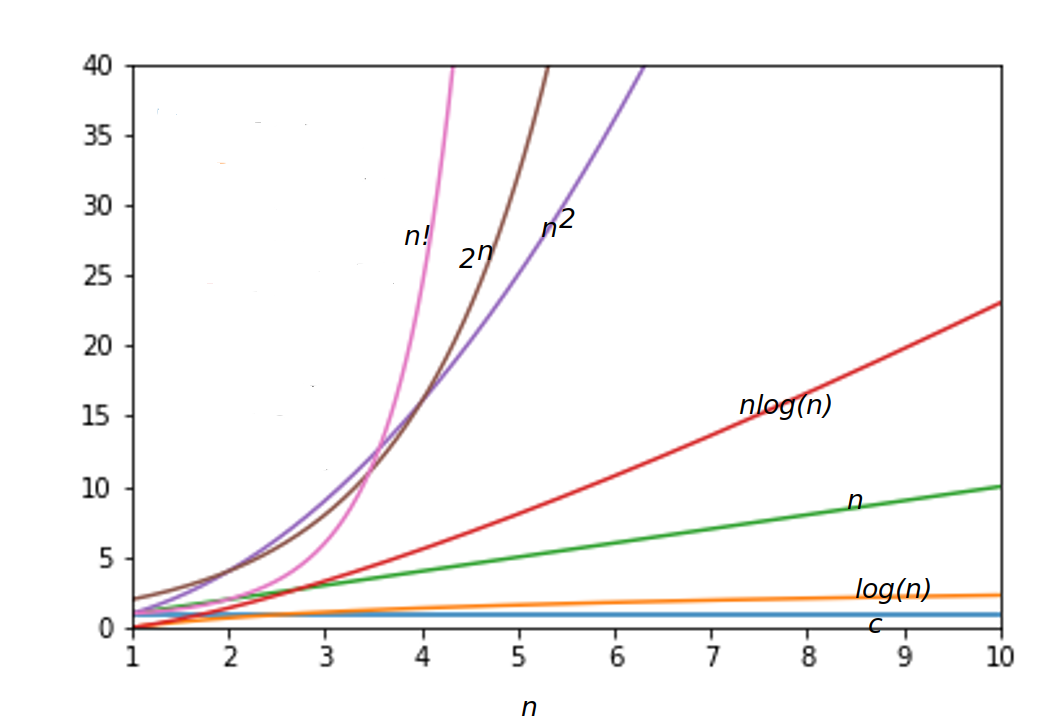
\includegraphics[width=170pt,height=130pt]{slike/growth.png}%growth-Functions.jpg}
   \caption{Grafik odnosa klasa $O$-složenosti.}  \label{fig:slozenosti_funkcije-a}
 \end{figure}


U praksi, neželjena složenost algoritma je eksponencijalna, dok su logaritamska, linearna i log-linearna složenost poželjne i takvi algoritmi su obično veoma efikasni u rješavanju problema, tj. instanci velikih dimenzija. U zavisnosti od tipa problema, kvadratna složenost može ali i ne mora biti garant za rješavanje realnih instanci većih dimenzija razmatranog  problema. %U najvećem broju slučajeva, klasa funkcija koja  koja prelazi kvadratnu je nedovoljno dobra. 


U nastavku izlažemo neka uputstva koja olakšavaju računanje složenosti algoritma. Za (pod)program $P$, označimo njegovu složenost izvođenja sa funkcijom $T(P)$ koja (direktno ili indirektno) zavisi od dimenzije ulaza ($n$). 
 
\begin{table}[H]
		\caption{Uputstva za računanje složenosti algoritma.}  \label{tab:uputstva_racunanje}
	\centering
	\begin{tabular}{l |l} \hline 
		\textbf{Konstrukcija}         & \textbf{Računanje složenosti} \\ \hline
		Jedinične instrukcije         & 1 \\
        Serija naredbi $S$: $N_1$; $N_2$; &  $T(S) = T(N_1) + T(N_2)$  \\ \hline
        Naredba grananja $S$:           &                                \\
        \textbf{IF}  $C$ then $N_1$ \textbf{ELSE} $N_2$  & $T(S) = T(C) + \max\{ T(N_1), C(N_2)\}$  \\          \hline                 
         Naredba petlje $S$:            &   $n$ -- maksimalan broj iteracija          \\
         1) \textbf{WHILE} $U$ \textbf{DO} $N_1$                 &     $T(S)= n \cdot (T(U) + T(N_1))$         \\ 
         2) \textbf{FOR} $i=j$ \textbf{to} $p$ \textbf{DO} $N_1$  &    $T(S)= n\cdot T(N_1)$     \\  \hline
         
	\end{tabular}
\end{table}

Odgovorimo sada na pitanja da li je jedan algoritam efikasniji od drugoga?
Upravo, odgovor nam daju notacije za složenost koje smo naučili u ovoj glavi, i to dvije najznačajnije: $O$ i $\Theta$--notacije. Kažemo da je jedan algoritam $X$ \textit{asimptotski efikasniji} od drugog algoritma  $Y$ akko sa porastom veličine ulaza u oba algoritma, vrijeme rada algoritma $X$ postaje kraće od vremena rada $Y$. To znači da $X$ pripada nižoj $O$--klasi složenosti od $Y$. %https://www.geeksforgeeks.org/algorithms-analysis-of-algorithms-question-16/ 
Prema tome, za velike ulaze, algoritam $X$ je uvijek biti bolji izbor od  algoritma $Y$ u smislu efikasnosti (vremena izvođenja). Međutim, za male ulaze moguće je da je $Y$ i dalje brži od $X$. Stoga se ne može reći da je $X$ uvijek bolji izbor za sve ulazne vrijednosti, već da će $X$ biti bolji izbor za sve ulaze osim eventualno malih ulaza.


U narednom primjeru dajemo jedan zadatak, rješavamo ga na dva načina, te izvodimo složenost oba programa.

\begin{example}
 \textit{{Problem nalaska (neprekidnog) podniza  maksimalne sume}}.  Od svih neprekidnih podnizova datog
 niza, naći onaj čija je suma elemenata najveća moguća. 
\end{example}
\begin{solution}
 
 Neka je dat ulaz $\texttt{a} = [1, 4, -2, 2, 10, -7, 1]$.  Jedan neprekidan podniz ovog niza je $[ -2, 2, 10 ]$ (početne pozicije 2, te završne pozicije 4), ali $[-2, -7, 10]$ nije neprekidan podniz. 
 
Koristimo se naivnim pristupom rješavanja problema. Definišimo $$S(i, j) := \max  \{ a[i], \ldots, a[j] \},$$

gdje je $S(i, i ) = a[i]$. 
Funkcija $S(i,j)$ računa sumu elemenata neprekidnog podniza niza \texttt{a}, sa početnom pozicijom  $i$, te završnom pozicijom $j$.
Za izračunavanje funkcije $S(i, j)$, potrebno je $j-i+1$ instrukcija, što definitivno pripada klasi $O(n)$. Da bismo riješili problem na ovaj način, 
treba da pozovemo funkciju $S(i,j)$ za svaki par $(i,j),  {i, j \in \{0, \ldots , n-1\},  i \leq j}$, a to je ukupno $\binom{n}{2} + n$ puta, što odgovara klasi složenosti $O(n^2)$. Dakle, složenost ovakvog algoritma je $O(n)\cdot O(n^2) = O(n^3)$ što je kubna složenost. 

Pokušajmo konstruisati ``pametniji'' algoritam. Iskoristimo činjenicu da postoji jasna rekurzivna zavisnost između vrijednosti dva susjedna $S(i,j)$ i $S(i, j+1)$, tj. da je $S(i, j+1) = a[j+1] + S(i, j)$, za $j \in \{i, \ldots, n-2\}$. Definišimo sada:
$$ S(i):= \max \{ S(i, i), S(i, i+1), \ldots, S(i, n-1)\}.$$

Izvršavanje funkcije $S(i)$ se odvija u linearnoj složenosti, tj. $O(n)$. Kako se ona poziva $n$ puta (za svako $i \in \{0, \ldots n-1\}$ po jednom), ukupna složenost ovog pristupa je $n \cdot O(n) = O(n^2)$, što je znatno efikasnije od prethodnog, naivnog, pristupa. 
 

\end{solution}



 
 
 \section{Prostorna složenost}
 
 %https://www.geeksforgeeks.org/g-fact-86
 
 Termin prostorna složenost se na mnogim mjestima pogrešno koristi asocirajući na pomoćni prostor.  \textit{Pomoćni prostor} je dodatni ili privremeni prostor koji koristi algoritam.
 
 \textit{Prostorna složenost} algoritma je ukupan prostor koji algoritam zauzima u odnosu na veličinu ulaza. Prostorna složenost   uključuje i pomoćni prostor i prostor koji koristi ulaz.
 
 Prostorna složenost se može posmatrati kao pandan koncepta vremenske složenosti. Za kreiranje niza veličine $n$, zahtijeva se dodatan prostor od $O(n)$. Za kreiranje dvodimenzionalnog niza veličine $n \times n$,  zahtijeva se $O(n^2)$ prostora.
 Napomenimo da prostorna složenost zavisi i od programskog jezika, kompajlera, pa  čak i mašine koja pokreće algoritam.
 
 
 Efikasnost algoritma uglavnom je definisana u odnosu na  dva faktora, korišteni prostor i vrijeme. ``Dobar'' algoritam je onaj koji koristi manje vremena i prostora; međutim, to nije moguće stalno postići. Zbog toga postoji kompromis između vremena i prostora. Ako želimo skratiti vrijeme izvršavanja algoritma, korišteni prostor se obično povećava. Slično tome, ako želimo smanjiti prostor, vrijeme izvršenja algoritma se obično povećava. %Dakle, treba napraviti kompromis između prostora i vremena.  
 
 
 \begin{example}
 	Posmatrajmo sljedeći pseudokod, te odredimo prostornu složenost datog 
 	programa. 
 	
 	
 	\begin{algorithm}[H]
 		\begin{algorithmic}[1]
 			\Procedure{pairSum}{x, y}   
 			\State	\textbf{return} $x+y$
 			\EndProcedure
 			
 		\end{algorithmic}
 	\end{algorithm}        
 	
 	
 	\begin{algorithm}[H]
 		\begin{algorithmic}[1]
 			\Procedure{addSequence}{n}
 			
 			\State $sum \gets 0$
 			\For{$i = 0 \text{ to } n-1$}
 			\State $sum \gets sum + \texttt{pairSum}(i, i+1)$
 			\EndFor
 			\State \textbf{return} \textit{sum}~
 			\EndProcedure
 			
 		\end{algorithmic}
 	\end{algorithm}
 	
 	Prostorna složenost procedure \textsc{AddSequence} je jednaka $O(1)$, bez obzira što se funkcija \textsc{pairSum} poziva $O(n)$ puta. Zašto?
 	
 	
 \end{example}
 
 
  \textbf{\textit{Napomena}}. U standardnom programiranju, podrazumijeva se korištenje 256MB prostora za određeni program. Dakle, kreiranje   niza veličine veće od $10^8$ nije dozvoljeno, jer je na raspolaganju data gornja granica za količinu memorije na  raspolaganju. Takođe, kreiranje  niza veličine veće od $10^6$ u tijelu funkcije nije moguće, jer je maksimalni prostor dodijeljen funkciji (u lokalnom steku) 4MB. Dakle, da bismo koristili niz veće veličine, potrebno je kreirati globalni niz.

\section{Pseudokod}

\textit{Pseudokod} je jednostavan prikaz implementacije algoritma u obliku anotacija i informativnog teksta napisanog na običnom jeziku. On nema sintaksu kao bilo koji programski jezik i stoga ga računar ne može kompajlirati ili interpretirati. % Često su algoritmi  predstavljeni pomoću pseudo kodova jer se mogu protumačiti bez obzira na znanje onog koji ga nasoji razumjeti. 
 Pseudokod, kao što sam naziv sugeriše, je reprezentacija k\^oda koja je prilagođena da ga razumiju i osobe bez velikog znanja o programiranju i algoritmima. Za razliku od pseudokoda, algoritam je organizirani   niz instrukcija koji rješava određen problem pri implementiranju u nekom programskom jeziku, te se kompajliranjem  ili interpretiranjem prevodi u mašinski k\^od kojeg mašina može da izvrši.

Prednosti korištenja pseudokoda su sljedeće. 
\begin{itemize}
	\item Poboljšava čitljivost i razumijevanje bilo kojeg pristupa kojim se rješava problem.
%	\item Predstavlja jedan od najboljih načina za  implementaciju algoritma.
	\item Djeluje kao spona između programa i dijagrama toka.
	\item Služi kao gruba dokumentacija, da bi se program mogao lakše razumjeti. U industriji je vođenje dokumentacije od suštinskog značaja i tu se potreba za pseudokodom pokazuje krucijalnim.
\end{itemize}
 
 
Glavni cilj pseudokoda je da nedvosmisleno objasni suštinu svakog dijela programa, čime se olakšava faza izgradnje k\^oda te smanjuje mogućnost pravljenja  grešaka u implementaciji algoritma.

Pisanje pseudokoda počinje razumijevanjem problema koji se rešava. Nakon  jasnog definisanja problema, slijedi razmatranje koraka koje treba preduzeti kako bi se došlo do rešenja. Te korake zatim zapisujemo uz pomoć  pseudokoda.

Nekoliko saveta u vezi prakse pisanja ``dobrog''  pseudokoda su:
\begin{itemize}
	\item Koristiti jasne i precizne nazive za promenljive i funkcije.
	\item Koristiti opise koji jasno ukazuju na to šta se dešava u svakom koraku algoritma. 
	\item Razmisliti o slučajevima u kojima algoritam može da se zaustavi i načinima na koje  se to može desiti.
	\item Koristiti odgovarajuće sintakse za kontrolne strukture kao što su petlje i uslovi: \texttt{if-else}, \texttt{for}, \texttt{while} petlje. Koristiti mehanizam uvlačenja naredbi koje se izvršavaju u okviru istog bloka, jer pomaže lakšem shvatanju kontrolnog mehanizma i izvršavanja odluka. Ovakva praksa u velikoj mjeri poboljšava čitljivost k\^oda. Pogledajmo u nastavku primjer jednog jednostavnog pseudokoda.
	
	\begin{minted}{C}
        
                tip = unos sa tastature
		if tip == "1"
		   ispiši odgovor "Unesen je broj 1"
		
		if tip == "2"
		   ispiši odgovor "Unesen je broj 2"
	\end{minted}
	
	\item Dakle, pseudokod nije potrebno pisati na potpuno programski način. Njegova svrha je jednostavnost i razumijevanje čak i za osobe kojima programiranje nije struka, stoga ne bi trebalo sadržati previše tehničkih detalja.
\end{itemize}

\begin{example} Napisati pseudokod za nalazak najvećeg elementa u nizu. \\
 \begin{minted}{C}
 Inicijalizuj najveći broj na prvi element niza.
 Proći sve preostale elemente niza: 
    Ako je trenutni element veći od trenutno najvećeg broja,
    postavi trenutni element kao novi najveći broj.
 Kraj petlje.
 Ispiši najveći broj.
 \end{minted}
 
\end{example}

U nastavku navodimo (koncizniji) pseudokod, koji rješava problema nalaska podniza  maksimalne sume na efikasniji način. Ovdje će biti korišten česten format koji je više tehnički, a i više upotrebljavan u literaturi. 
 
 

 \begin{algorithm}[!ht]
 	\caption{Funkcija $S_i(i)$}\label{S_i}
 	\begin{algorithmic}[1]
 		\Procedure{S}{$i$, $niz$}
 		\State $s_{maxi}, s_{next} \gets niz[i]$
 		\For{$j=i+1$ to $n-1$}
 		\State $s_{next} \gets s_{next} + niz[j]$
 		\If{$s_{next} > s_{maxi}$}
 		\State $s_{maxi} \gets s_{next}$
 		\EndIf
 		\EndFor  
 		\State \Return $s_{maxi}$
 		\EndProcedure
 	\end{algorithmic}
 \end{algorithm}



\begin{algorithm}[H]
	\caption{Funkcija $S$}\label{S}
	\begin{algorithmic}[1]
		\Procedure{S}{$niz$}
		\State $s_{max}\gets niz[0]$ 
		\For{$i=0$ to $n-1$}
		\State $s_i \gets  S_i(i)$ 
		  \If{$s_{max} <  s_{i}$}
		    \State $s_{max} \gets s_{i}$
		  \EndIf
		\EndFor  
		\State  \Return  $s_{max}$
		\EndProcedure
	\end{algorithmic}
\end{algorithm}

\section{O valjanosti algoritma}

Postoji nekoliko načina da se formalno provjeri valjanost algoritama; tri  su osnovna načina:

\begin{itemize}
	\item \textit{Matematički dokaz}. Predstavlja jedan od najrigoroznijih načina za provjeru valjanosti algoritma.  %je matematički pokazati da algoritam uvijek daje ispravan izlaz. 
	Ovdje se koriste matematičke tehnike za analizu logike algoritma i za utvrđivanje da algoritam radi ispravno za sve moguće ulaze. Jedana od metoda je \textit{metoda invarijantne petlje}, kojom ćemo se pozabaviti u nastavku ove sekcije. 
	
    \item \textit{Formalna verifikacija}. Formalna verifikacija je proces upotrebe matematičkih tehnika i alata za provjeru da li algoritam ispunjava određene specifikacije. Ovo uključuje modelovanje algoritma korištenjem formalnog jezika, a zatim korištenje automatiziranih alata za provjeru da li model zadovoljava određena svojstva. U osnovi, ovi metodi su iz domena vještaške inteligencije specijalno namijenjeni za verifikaciju softvera.
    \item \textit{Testiranje}.  Iako testiranje nije formalna metoda već \textit{empirijska}, ona predstavlja važan način za provjeru valjanosti algoritma. Pokretanjem algoritma sa raznim ulaznim vrijednostima i provjeravanjem izlaza u odnosu na očekivane rezultate, može se steći povjerenje o tome da li je algoritam ispravan.

\end{itemize}


Metoda \textit{invarijantne petlje} (eng. \textit{{loop} {invariant}}) predstavlja jednu od matematičkih tehnika koja se koristi u dokazivanju ispravnosti algoritama. Invarijanta petlje je tvrdnja koja ostaje istinita tokom svake iteracije petlje programa, uključujući i prije i poslije izvršavanja naredbi u iteraciji.

Da bismo koristili metod invarijantne petlje u dokazivanju ispravnosti algoritma, najčešće se kombinuju sljedeći koraci.

\begin{itemize}
	\item  Definisanje invarijante petlje: potrebno je definisati tvrdnju koja ostaje istinita prije i poslije svake izvršene iteracije petlje.
   \item Dokazivanje inicijalne invarijante: treba pokazati da je invarijanta petlje istinita prije prve iteracije petlje.
   \item Dokazivanje održavanja invarijante: potrebno je dokazati da ako je invarijanta istinita prije određene iteracije petlje, onda je istinita i nakon izvršavanja te iteracije.
   \item Dokazivanje da se petlja završava: pokazati da se nakon konačnog broja iteracija, petlja prekida.
   \item Dokazati da algoritam rješava problem: potrebno dokazati da, ako je invarijanta istinita, nakon posljednje iteracije petlje, algoritam uistinu rješava problem.
\end{itemize}

Ova metoda je korisna u dokazivanju ispravnosti algoritama koji se sastoje od petlji, jer omogućava dokazivanje da algoritam radi ono što je i očekivano, tj. da ispravno rješava problem za sve moguće ulaze.

\begin{example}
Demonstrirajmo   pokazivanje ispravnosti programa za nalazak \textit{najvećeg zajedničkog djelioca (NZD)} dva prirodna broja, datog   Algoritmom~\ref{alg:nzd}, uz pomoć metoda invarijantne petlje.


\begin{algorithm}
	\begin{algorithmic}[1]
		\Procedure{NZD}{$n, m$}
		\State $nzd \gets \min(n, m)$
		\While{!($n \% nzd == 0 \  \& \ m \% nzd == 0$)}
		    \State $nzd \gets nzd - 1$
		\EndWhile
		\State \Return $nzd$
		\EndProcedure
	\end{algorithmic}
   \caption{NZD dva broja.} \label{alg:nzd}
\end{algorithm}

Ovaj program je konačan, jer je broj iteracija u glavnoj \emph{while}-petlji najviše $nzd$, dok je broj instrukcija u svakoj iteraciji takođe konačan (jednak 5+2=7). Dalje, odredimo uslov invarijantne petlje. Neka je ${nzd}^*$ konačan rezultat koji program vraća (koji je zasigurno zajednički djelilac, po uslovu prekida petlje). Tada  invarijantnu petlju definišemo sa 
$$ nzd^* \leq nzd.$$

Prije ulaska u prvu iteraciju petlje imamo $nzd^* \leq nzd = d_0 = \min(n, m)$. 
Neka je prije ulaska u $k$-tu iteraciju petlje $d_{k-1} = nzd$. Tada je  $nzd^* < d_{k-1}$ jer se  ulaskom u $k$-tu iteraciju petlje uvjeravamo da $d_{k-1}$ ne može biti NZD ulaznih brojeva (jer tada zadovoljava uslov \textit{while}-petlje). Tada imamo $d_{k} = d_{k-1} -1 \geq nzd^*$ nakon završetka $k$-te iteracije, čime je uslov invarijantne petlje i tada zadovoljen.   Pretpostavimo da se u iteraciji $k^*$ program prekida. To znači da je $d_{k^*-1}$ zasigurno zajednički djelilac. Kako tražimo najveći takav, onda je i $d_{k^*-1} \leq nzd^*$. S obzirom da je  $d_{k^*-1} \geq nzd^*$ zbog uslova invarijantne petlje, slijedi da je 
$d_{k^*-1} = nzd^*$, čine smo pokazali valjanost algoritma.
\end{example}
Pokazivanje valjanosti kompleksnih algoritama pomoću metoda invarnijantne petlje je rijetko  praktično. Jedan od razloga je taj što definisanje samog uslova invarijantnosti nije trivijalan zadatak, kao  i to da instrukcije koje se izvršavaju u svakoj iteraciji nisu trivijalne  (kao što je to slučaj sa prethodnim programom), te mogu uključivati  pozivanje složenijih pomoćnih funkcija. U takvim slučajevima, valjanost algoritma provjeravamo empirijski, izvršavajući ga nad instancama različitih veličina i distribucija te provjeravajući  validnost vraćenih rezultata (za instance za koje znamo tačan rezultat, dok za one za koje ne znamo, provjeravamo ispunjivost uslova zadatka). 

\section{Euklidov algoritam: složenost}
Klasični algoritam za nalazak NZD je Euklidov algoritam, dat Algoritmom~\ref{alg:nzd-euclid}. On predstavlja jedan od najpoznatijih algoritama u polju aritmetike. Izvedimo njegovu vremensku složenost. 

\begin{algorithm}
	\begin{algorithmic}[1]
		\Procedure{NZD}{$p, q$}  \# pretpostavka je da $p \geq  q$
		\State $x \gets p$ 
		\State $y \gets q$
		\While{ $y > 0 $}
		\State $ x \gets y  $
		\State $y \gets x \% y $
		\EndWhile
		\State \Return $x$
		\EndProcedure
	\end{algorithmic}   \caption{NZD dva broja.} \label{alg:nzd-euclid}
\end{algorithm}

\begin{example}
	Prvo izvedimo korake algoritma na konkretnoj instanci. Neka je $p=400$, a $q=24$. Tada imamo korake:
	$$(400, 24) \rightarrow (24, 16) \rightarrow (16, 8) \rightarrow (8, 0),$$
	odakle slijedi da je NZD$(400, 24)=8$. Za razliku od naivnog algoritma za nalazak NZD iz prethodnog poglavlja, koji bi za ovu instancu izveo 17 iteracija do nalaska rješenja, vidimo da za Euklidov algoritam treba svega 4 iteracije da nađe tačno rješenje. 
	
	Prvo, Euklidov algoritam je konačan, jer je broj iteracija ograničen sa $\min(p, q)$. Drugo, algoritam ne zavisi direktno od veličine ulaza (koji je konstantan, tj. veličine $2=|\{p, q\}|$), već od veličine brojeva, ili dužine binarne reprezentacije (dekadnih) brojeva u ulazu. Ako je $p$ broj u dekadnom zapisu, dužina njegovog binarnog zapisa jednaka je $\lfloor \log_2(p) \rfloor+1$. Dalje, označimo sa $n_1$   broj bitova u zapisu broja $p$, a sa $n_2$  broj bitova u zapisu broja $q$. 
	Tada je
	$$n_1 \approx \log_2(p), n_2 \approx \log_2(q),  n = n_1 + n_2 = \log_2(p \cdot q ).$$
	
	Vrijednost $n$ je najveća kada su $p$ i $q$ susjedni brojevi, odakle je $ n_1 \approx n_2 \approx n/2$,  pa za složenost algoritma $T(n)$ vrijedi da je proporcionalna vrijednosti manjeg od
	ta dva broja.  
	Dakle, imamo $T(n)  = \Omega(q) = \Omega(2^{n_2}) =  \Omega(2^{n/2})$.
	
	U svrhu pokazivanja složenosti, iskoristimo sljedeću teoremu, koju i formalno dokazujemo. 
	\begin{theorem}
		 Za svaka dva broja $p$ i $q$ vrijedi
		 $$ x \% y \leq x / 2.$$
	\end{theorem}
	 
	 \begin{proof}
	 	Razlikujemo dva slučaja:
	 	\begin{itemize}
	 		\item $x/2 < y \Rightarrow$  $x\%y = x  - y  \leq x/2 $;
            \item $x/2 \geq  y\Rightarrow$ $x\% y < y \leq x / 2$.
	 	\end{itemize}
	 \end{proof}
	
Procijenimo broj koraka algoritma. Algoritam izvodi sljedeći niz koraka:

$$(p_0,  q_0 ) \rightarrow (p_1, q_1) \rightarrow \cdots \rightarrow (p_m,q_m ) \rightarrow (p_{m+1}, q_{m+1}=0),$$	
	
	gdje je $p_0 = p, q_0 = q$, nakon čega algoritam prekida sa radom. Procijenimo vrijednost broja koraka $m$. 
	
	Imamo: $p_1 = q_0, q_1 = p_0 \%q_0. $ Dalje, primjenom prethodne teoreme imamo: 
	$$ p_1 q_1 = q_0 p_0 \% q_0  \leq q_0 p_0 /2.$$
	
	Slično je 
		$$ p_2 q_2 \leq q_0 p_0 /2^2 .$$
Takođe je 
		$$ 1  \leq p_m q_m \leq q_0 p_0 /2^m, $$
odakle dobijamo $pq =  q_0 \cdot p_0 \geq 2^m, $ odakle nakon primjene logaritma dobijamo 

$$   m < \log (pq ) = n,$$

odakle imamo $m = O(n)$.

U svakom koraku algoritma, najskuplji korak je računanje modula, za koji je neophodno dijeljenje dva binarna broja. Taj proces zahtjeva $O(n^2)$ instrukcija. 
Iz svega imamo da je složenost algoritma:
$$ O(n^2)\cdot O(n) = O(n^3)= O(\log \max\{p,q\}).$$

Primijetimo da je prostorna složenost Euklidovog algoritma konstanta, tj. jednaka je $O(1)$. 
\end{example}


Napomenimo da valjanost Euklidovog algoritma slijedi iz algebarskog svojstva da je skup djelilaca brojeva $p$ i $q$, jednak skupu djelilaca brojeva $q$ i $p\%q$, pa su stoga transformacije parova brojeva za koje se razmatra NZD u svakom koraku validne, dok se ne dođe od trivijanog slučaja, tj. dok drugi broj ne bude jednak nuli, čime se vraća vrijednost prvog broja kao krajnji rezultat. 

Kako smo vidjeli, iako je Euklidov algoritam relativno jednostavnog k\^oda, njegovu složenost nije bilo trivijalno odrediti. Napomenimo da Euklidov algoritam predstavlja jedan vid rekurzivnog algoritma.  %, gdje rekurzija u tijelu funkcije poziva samu sebe, ali sa ulazom manje veličine. 
 U osnovi, za računanje složenosti ovakvih algoritama, o kojima će biti više riječi u Glavi 3, koristi se poznata Master teorema. Ovu teoremu navodimo bez dokaza, uz napomenu da se ona navodi i formalno dokazuje na nekim od kurseva algoritmike na višim godinama studija. Mi ćemo je koristiti isključivo samo kao pomoćni alat u već pomenutoj Glavi 3, kod određivanja složenosti algoritama nekih problema koje budemo rješavali. 

\begin{theorem}[Master teorema]
	Neka je data jednačina 
$$T(n) = aT\left(\frac{n}{b}\right) + f(n)$$
gdje je  $n$  veličina ulaza, broj $a$ predstavlja  broj podproblema,
$n/b$ veličinu svakog podproblema, $f(n)$ broj instrukcija koji je potreban pored rekurzivnog poziva, uz $a\geq 1$ i $b>1$, dok je $f(n)\geq 0$. Vrijedi sljedeće:
\begin{itemize}
	\item Ako je $f(n) = O(n^{\log_b (a) - \epsilon})$ za neki $\epsilon>0$, onda $ T(n) = \Theta (n^{\log_b (a)})$;
	\item Ako je $f(n) = \Theta (n^{\log_b (a)})$, onda je $T(n) = \Theta (n^{\log_b (a)} \log(n))$;
	\item Ako je $f(n) = \Omega (n^{\log_b (a) + \epsilon})$  za neki $\epsilon>0$, onda je $T(n) = \Theta (f(n))$. 
	
\end{itemize}
\end{theorem} 

Na sljedećim primjerima pokazujemo kako funkcioniše primjena Master teoreme. %https://iq.opengenus.org/master-theorem-time-complexity/
 

\begin{example}
	Posmatrajmo formulu:
	$$T(n) = 2T\left(\frac{n}{2}\right) + n.$$
	Kako je $a = 2, b = 2, f(n) = n$, te $f(n) = n = n^{log_b (a)} = n^{\log_2 (2)} = n$, iz Master teoreme, na osnovu slučaja 2,  možemo zaključiti da je 
	$$T(n) = \Theta (n^{\log_b (a)} \log (n)) = \Theta (n \log n).$$
\end{example}

\begin{example} Neka je data formula
	$T(n) = T(\frac{n}{2}) + O(1)$
	Imamo $a = 1, b = 2, f(n) = 1$, pa je $$f(n) = 1 = n^{\log_b (a)} = n^{\log_2 (1)} = n^{0} = 1.$$
	Na osnovu Master teoreme, slučaj 2, imamo
	$$T(n) = \Theta (n^{\log_b (a)} \log (n)) = \Theta (\log n).$$
\end{example}

\begin{example}
	Neka je data sljedeća rekurzija:
	$$T(n) = T(\frac{n}{2}) + cn, c >0.$$
	
	Imamo $a = 1, b = 2, f(n) = cn$, pa je 
	$$f(n) = cn = n^{\log_b (a)} = n^{\log_2 (1) + \varepsilon} = n^{\varepsilon} \text{ za neki } \varepsilon \leq 1.$$
	
	Na osnovu Master teoreme, slučaj 3, imamo % $$ah(\frac{n}{b}) = \frac{cn}{2} = \frac{1}{2}h(n)$$ 
	%pa je 
	$T(n)  = \Theta (cn) = \Theta(n).$
\end{example}

\section*{Zadaci}

\begin{enumerate}
	\item Izračunati vremensku složenost sljedećeg programa:
	
	\begin{algorithm}[H]
		\begin{algorithmic}[1]
		\Procedure{Zad1}{$N$}
		    \State $ a \gets  0$
		    \For{$i = 0 \text{ to } N$}
		         \For{$j = N \text{ downto } i$}
		    		\State $a \gets  a + i + j$
		         \EndFor
		     \EndFor
	    \EndProcedure	 	    
		\end{algorithmic}
	\end{algorithm}
\item Izračunati vremensku složenost sljedećeg programa 
	\begin{algorithm}[H]
	\begin{algorithmic}[1]
	 \Procedure{Zad2}{$n$}
		\State $i, j, k \gets  0$
		\For{$i = n / 2 \text{ to } n$}
			\For{$j = 2; j \leq n; j = j * 2$}
				\State $k \gets  k + n / 2$
			\EndFor
		\EndFor
	\EndProcedure	 
	\end{algorithmic}
\end{algorithm}
 \item Izračunati vremensku složenost sljedećeg programa 

	\begin{algorithm}[H]
	\begin{algorithmic}[1]
     \Procedure{Zad3}{$N$}
		\State $a \gets 0, i \gets N$
		\While{$i > 0$}
			\State $a \gets a+ i$
			\State $i \gets i / 2$
		\EndWhile
    \EndProcedure	 
	\end{algorithmic}
\end{algorithm}
 \item Izračunati vremensku složenost sljedećeg programa 

\begin{algorithm}[H]
	\begin{algorithmic}[1]
	 \Procedure{Zad4}{$n$}
		\State $k \gets 3$
		\For{$i=0 \text{ to } n-1$}
		    \State $i \gets i * k$
		\EndFor
	   \EndProcedure
	\end{algorithmic}
\end{algorithm}

 \item Izračunati vremensku složenost sljedećeg programa 

\begin{algorithm}[H]
	\begin{algorithmic}[1]
	\Procedure{Zad5}{$n$}
	  \State $sum \gets 0$
	  \For{$i = 1 \text{ to } n$}
	      \For{$j = 1 \text{ to } i\cdot i$}
	          \If{$j \text{ mod } i == 0$}
	              \For{ $k = 1 \text{ to } j$}
                      \State	$sum \gets sum + 1$
                 
                  \EndFor
              \EndIf
          \EndFor
     \EndFor
    \EndProcedure
	\end{algorithmic}
\end{algorithm}


 
 \item Izračunati (ukupnu) složenost sljedeće rekurzije:

\begin{algorithm}[H]
	\begin{algorithmic}[1]
		\Procedure{bubbleSort}{$arr[],size$}
        \For{$i = 0; i < size-1; ++i$}
 	        \For{$j = 0; j < size-1; ++j$}
 	  
 	 	      \If{$arr[j] > arr[j+1]$}
 		        \State $swap( arr [j] , arr [j+1] )$
 		      \EndIf
 		   \EndFor
 	    \EndFor
		\EndProcedure
	\end{algorithmic}
\end{algorithm}



 
	 
 \item Izračunati složenost sljedeće rekurzije: %https://www.geeksforgeeks.org/analysis-algorithms-set-5-practice-problems/?ref=rp
  
 $$	T(n) = 
 \begin{cases}    
         &3\cdot T(n-1), \text{ako }  n > 0 , \\
         & 1, \text{inače} 
   \end{cases}$$

  \item Izračunati složenost sljedeće rekurzije:

$$	T(n) = 
\begin{cases} 
  		&2T(n-1) - 1, \text{ako } n>0, \\
		& 1, \text{inače}
\end{cases}
$$

\item Izračunati prostornu složenost programa datog sljedećim pseudokodom
%https://www.prepbytes.com/blog/data-structure/space-complexity/

\begin{algorithm}[H]
	\begin{algorithmic}[1]
		\Procedure{sum}{$arr[],N$}
		
		\State  $ans \gets 0$
		\For{$i = 0 \text{ to } N$}
		\State $ans \gets ans+arr[i]$
		\EndFor
		\State ispiši $ans$
		\EndProcedure
	\end{algorithmic}
\end{algorithm}



\item Izračunati prostornu složenost programa datog sljedećim pseudokodom
%https://www.prepbytes.com/blog/data-structure/space-complexity/
 
\begin{algorithm}[H]
	\begin{algorithmic}[1]
	  \Procedure{faktorijel}{$N$}
	  	\State $fact \gets 1$
	  	 \For{$i=1 \text{ to } N $}
	  	   
	  	   \State	$fact \gets fact * i$
	  	 \EndFor
	  	\State \textbf{return} \textit{fact}
	  \EndProcedure
	\end{algorithmic}
\end{algorithm}
 


\end{enumerate}
\chapter{Uvod u programski jezik Pajton} 
 

Pajton je objektno-orjentisani programski jezik visokog nivoa,  opšte   namjene,   pušten u upotrebu u februaru 1991. godine. Kreiran je od strane Guido van Rossum-a. Naziv Pajton potiče od britanske komičarske grupe \textit{Monty Python}. Od svog nastanka, Pajton je imao nekoliko  izdanja; danas je jedan od najpopularnijih programskih jezika na svijetu, pogledajte Sliku~\ref{fig: popular_program_lang}\footnote{Podaci preuzeti sa  https://statisticsanddata.org/data/the-most-popular-programming-languages-1965-2022-new-update/ .}.

\begin{figure}[H]
	\centering
	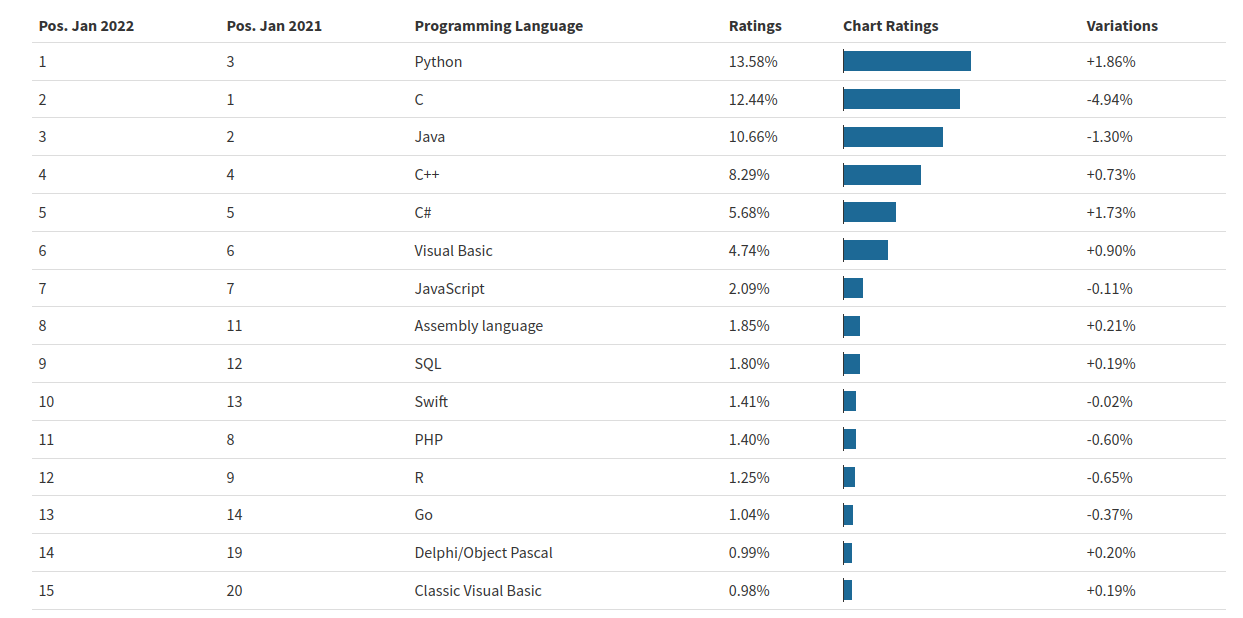
\includegraphics[width=380pt,height=190pt]{slike/most_popular_language.png}
	\label{fig: popular_program_lang}
	\caption{Statistički pregled najpopularnijih programskih jezika (godina 2021--2022). }
\end{figure}

U nastavku navodimo nekoliko važnih informacija vezanih za istoriju razvoja programskog jezika Pajton. 
 
Godine 1989. Guido van Rossum je samoinicijativno započeo rad na kreiranju novog programskog jezika kao poboljšanoj verziji ABC jezika, koji se uglavnom koristio za podučavanje osnovama  programiranja. Van Rossom je izgradio Pajton uzimajući po njemu pozitivne strane ABC jezika kao bazu, a poboljšavajući ili iznova implementirajući lošije koncepte tog jezika. 

 Prva verzija Pajtona, verzija 0.9.0, je objavljena  u februaru 1991. godine.
Pajton 1.0 je objavljen u januaru 1994. godine.  Uključio je nekoliko novih funkcionalnosti, preuzimajući uglavnom dobre koncepte funkcionalnih jezika, kao što su lambda, mapa, filter i funkcije redukcije.
Pajton 2.0 je objavljen 2000. godine i uveo je komprehenziju liste, sakupljač otpadaka i mnoga druga poboljšanja.
Pajton 3.0 je objavljen 2008. godine kao veliko ažuriranje koje je uključilo nekoliko izmjena koje nisu bile kompatibilne sa prethodnim verzijama. \\ 

Glavna odlika verzije Pajton 3.0 bio je pročišćavanje jezika i uklanjanje redudantnih funkcija.
Od pojavljivanja Pajton 3, tim zadužen za razvoj pajtona pušta glavne verzije jezika svakih 18-24 mjeseca. Svaka nova verzija uključuje nove funkcije i poboljšanja, čuvajući kompatibilnosti sa prethodnim verzijama.
Danas se Pajton koristi u gotovo svemu, od razvoja veb aplikacija, do naučnog računarstva, analize podataka, vještačke inteligencije, mašinskog učenja itd. Prednost 
Pajtona je velika i aktivna zajednicu programera koja   svakodnevno doprinose  jeziku kreiranjem biblioteka, frejmvorka i drugih alata. Neke od popularnih biblioteka i frejmvorka za Pajton uključuju NumPy, Pandas, Matplotlib, Django, TensorFlow.


Razvoj Pajtona karakteriše njegova sintaksna jednostavnost, čitljivost i fleksibilnost. Ovi aspekti su pomogli  da Pajton postane popularan jezik među početnicima ali i iskusnijim  programerima.

\section{Osnovne karakteristike}
%Osnovne karakteristika programskog jezika Pajton su: 

\begin{itemize}
	\item Pajton je \textit{jezik visokog nivoa} (eng. \textit{high-level language}):  programski jezik koji je dizajniran tako da ga ljudi lako čitaju, pišu i razumiju. U prevodu,  obezbjeđuje koncepte koje omogućavaju pisanje k\^oda na višem nivou apstrakcije, čime ga približava sintaksi prirodnog jezika, za razliku od jezika niskog nivoa, kao što su asemblerski ili mašinski k\^od.
	\item Pajton je \textit{dinamički tipizirani jezik}. To znači da  se tip varijable određuje u vrijeme izvođenja programa, a ne u vrijeme kompajliranja ili kodiranja. Drugim riječima, tip varijable se može promijeniti tokom izvršavanja programa. Nasuprot ovome, statički tipiziranim jezicima,  tip varijable je fiksiran u vrijeme kompajliranja i nepromjenljiv je tokom vremena izvršavanja. U statički tipiziranim jezicima,  tip svake varijable se mora deklarisati prije upotrebe, a potom kompajler provjerava da li se tip varijable dosljedno upotrebljava u cijelom programu.
	\item Pajton je \textit{objektno-orijentisani jezik}.  Objektno orijentisani programski (OOP) jezik  je tip programskog jezika koji koristi objekte kao svoje osnovne gradivne blokove. Objekti su instance klasa koje enkapsuliraju podatke i operacije (metode) koje se mogu izvršiti na tim podacima. U osnovi,  OOP koncept potiče prirodniji način razmišljanja o problemima tako što ih modeluje u smislu objekata i njihovih interakcija.
	\item Pajton je \textit{skriptni jezik}. Programski jezik koji je dizajniran dijelom za  skriptiranje,   pisanja tipa programa koji se koristi za automatizaciju zadataka, kao što je izvođenje niza naredbi ili manipulaciju podacima. Skriptni jezici se obično interpretiraju, a ne kompajliraju, što znači da se izvorni kod može izvršiti direktno, bez prethodnog prevođenja u mašinski k\^od.  	Jezici za skriptiranje se često koriste za   automatizacija zadataka koji se ponavljaju, pisanje malih potpornih programa ili ugrađivanje funkcionalnosti u drugim aplikacijama. Jedna od glavnih prednosti skriptnih jezika je njihova jednostavnost upotrebe i fleksibilnost.
	\item Pajton posjeduje \textit{aitomatsko čišćenje memorije} (eng. \textit{garbage--collected} language).  Pajton automatski upravlja   identifikovanjem i oslobađanjem memorije koju program više ne koristi.  Oslobađena memorija  stavljanja se na raspolaganje drugim dijelovima programa za korištenje.   Ovaj mehanizam omogućuje  programerima  da se usredotoče na pisanje koda bez vođenja brige o ručnom dodeljivanju i oslobađanju memorije (dok to nije slučaj u, recimo, programskom jeziku $C$).
\end{itemize}

\section{Pregled ugrađenih tipova podataka}

Pajton nudi nekoliko \textit{ugrađenih} (eng. \textit{built-in}) tipova podataka koji su dio osnovnog jezika. Oni su dostupni bez potrebe za dodatnom instalacijom ili bibliotekama. Među ugrađeni tipovima podataka (koji predstavljaju klase), od naročite bitnosti su sljedeći tipovi:

\begin{itemize}
	\item  numerički tipovi: \texttt{int}, \texttt{float}, \texttt{complex};
	 \item  tekstualni sekvencijalni tipovi: \texttt{str}, \texttt{bytes}, \texttt{bytearray};
	\item  sekvencijalni tipovi: \texttt{list}, \texttt{tuple}, \texttt{range}; 
	\item  mapirajući tipovi: \texttt{dict};
	\item skupovni tipovi: \texttt{set}, \texttt{froznenset};
	\item  boolean tip: \texttt{bool};
	\item  binarni tipovi: \texttt{memoryview}.
\end{itemize}


Svaki od ovih tipova posjeduje različite funkcionalnosti za skladištenje i manipulaciju podacima, te se koriste za kreiranje složenih struktura podataka i algoritama. Osim toga, Pajton pruža širok raspon biblioteka koje proširuju funkcionalnost ovih ugrađenih tipova, time omogućavaju kreiranje moćnih i fleksibilnih aplikacija sa lakoćom.

\section{Deklarisanje varijabli i memorijska organizacija}

Dodjela vrijednosti varijablama se izvršava pomoću operatora (dodjele) ``='', kao i kod većine programskih jezika. Da bismo kreirali varijablu, prvo odaberemo naziv varijable, a potom joj dodijelimo vrijednost pomoću operatora ``=''. Npr. za kreiranje varijable pod nazivom \textit{x} sa vrijednošću   5, koristimo sljedeći kod:

\begin{minted}{python}
	x = 5
\end{minted}

Da bismo kreirali varijablu pod nazivom \textit{y} i dodijelili joj stringovnu vrijednost ``abc'', napišemo:
\begin{minted}{python}
	y = "abc"
\end{minted}

Više o cjelobrojnim i stringovnim tipovima podataka biće riječi u nastavku. 
 
Pajton je objektno-orjentisani jezik, gdje se svaka varijabla tretira kao objekat neke klase.  
Objekti koji su varijable sa cjelobrojnom vrijednošću se tretiraju kao objekat tipa \texttt{int}. Dalje, varijabla koja je referencirana na string se tretira kao objekat tipa \texttt{str}.  Inače, gledajući memorijsku organizaciju, pojednostavljeno govoreći, varijable pretstavljaju reference na memorijsko mjesto gdje je upisan sadržaj na koji referenciraju.  
%https://www.analyticsvidhya.com/blog/2021/05/why-you-should-avoid-using-python-lists/
Detaljnije, pajtonov interpreter (o kome će biti više riječi u nastavku) je   napisan u \textit{C}-u, pa su svi pajtonovi objekti prikrivena verzija \textit{C} struktura, stoga  sadrže ne samo svoju vrijednost, već i druge informacije. Objekat nije samo sirovi cijeli broj (ili string ili drugi tip podatka), već pokazivač na složenu \textit{C} strukturu (npr. \texttt{PyLongObject}) koja sadrži nekoliko vrijednosti. Ako istražimo dublje, možemo vidjeti kako ova \textit{C} struktura izgleda.

\begin{minted}{C}
	struct _longobject {
		long ob_refcnt;
		PyTypeObject *ob_type;
		size_t ob_size;
		long ob_digit[1];
	};
\end{minted}
gdje je
\begin{enumerate}
	\item   \textit{\textit{ob\_refcnt}} -- brojač referenci koji upravlja dodjelom i oslobađanjem memorije.
    \item \textit{ob\_type} -- tip varijable.
    \item  \textit{ob\_size} -- veličina podatkovnih članova.
    \item  \textit{ob\_digit} -- čuva stvarnu vrijednost koju varijabla predstavlja.
\end{enumerate}

Sve ove dodatne informacije iziskuju   dodatne troškove u smislu memorijskih i računarskih resursa. Stoga je pajtonov  objekat (nekog tipa podatka)  ništa drugo nego pokazivač na poziciju u memoriji koja sadrži sve informacije o toj varijabli, uključujući količinu memorije sa stvarnom vrijednošću   tog tipa.  Dakle, sve ove dodatne informacije su ono što omogućuje da slobodno kodiramo u pajtonu, bez vođenja brige o tipovima podataka varijabli. Ipak, navedimo da se tip varijable može eksplicitno dodijeliti, kao u narednom primjeru
\begin{minted}{python}
	 x: str = "abc" 
	 y: int = 23
\end{minted}


Jednostavnosti radi, sljedeći k\^od
\begin{minted}{python}
    x = 42
\end{minted}
 pojednostavljeno možemo predstaviti sljedećom vizuelizacijom:
\begin{figure}[H]
	\centering
   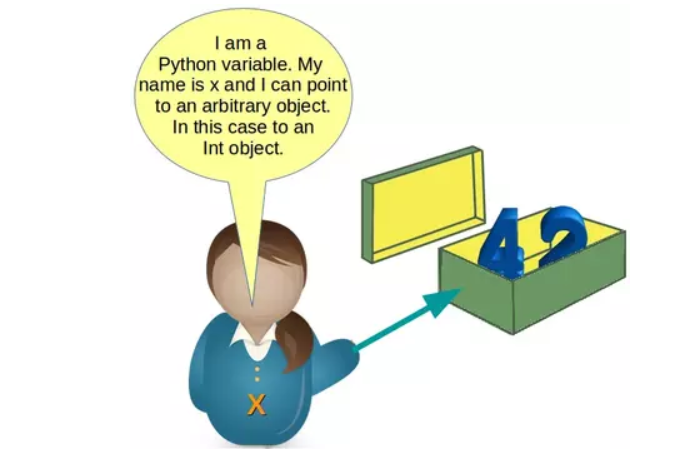
\includegraphics[width=140pt,height=100pt]{slike/variable_object.png}
\end{figure}
U slučaju da dodamo sljedeću liniju   koda 
\begin{minted}{python}
	y = x
\end{minted}
dobijamo situaciju    koja odgovara slici

%point_two_vars.png
\begin{figure}[H]
	\centering
	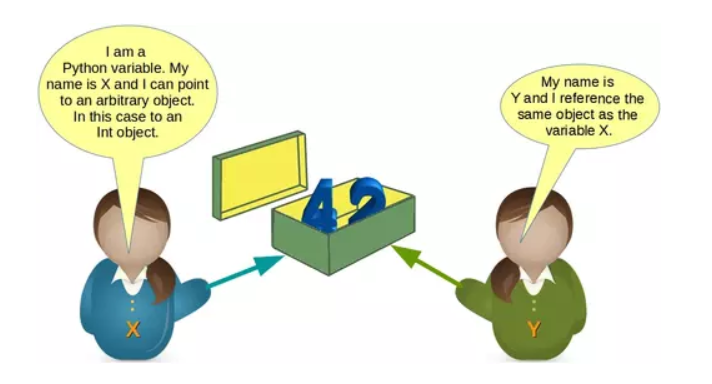
\includegraphics[width=140pt,height=100pt]{slike/point_two_vars.png}
\end{figure}
U slučaju da dodamo sljedeću liniju koda na prethodni k\^od
\begin{minted}{python}
	x = 72
\end{minted}
dobijamo sljedeći prikaz
\begin{figure}[H]
	\centering
	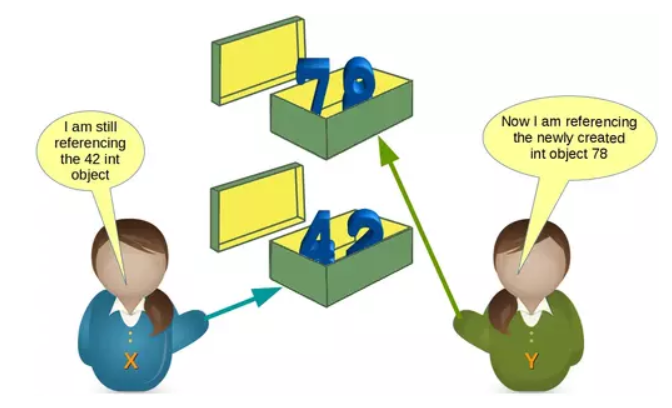
\includegraphics[width=140pt,height=100pt]{slike/vars_different_assigned.png}
\end{figure}
Konačno, ako postavimo y na novu vrijednost, tj.
\begin{minted}{python}
	x = "abcd" 
\end{minted}
imamo odgovarajuću sliku 

\begin{figure}[H]
	\centering
	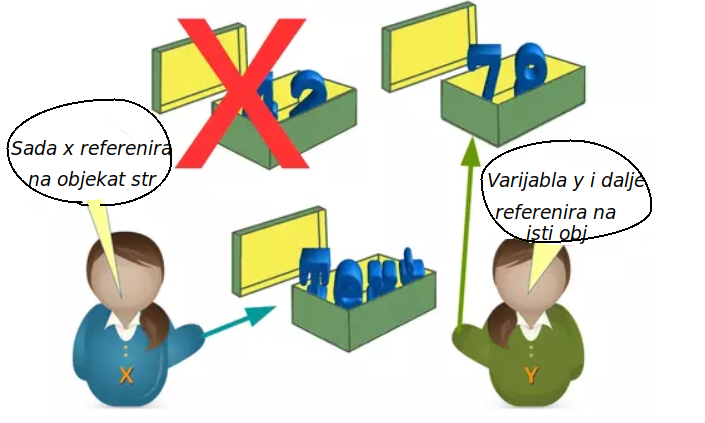
\includegraphics[width=140pt,height=100pt]{slike/varX_different_assigned.png}
\end{figure}

Primijetimo da na memorijsko mjesto gdje je broj 42 bio upisan ne pokazuje niti jedan pokazivač.  Pajton koristi tehniku zvanu \textit{brojač referenci} (atribut \textit{ob\_refcnt}) za upravljanje memorijom. Za svaki objekt, uključujući i složenije strukture kao što su kolekcije, vezuje se jedan broj referenci koji prati broj referenci na objekt. Kada referentni broj postene nula, objekt se briše iz memorije uz pomoć sakupljača otpadaka (eng. \textit{garbage collector}).

Sakupljač otpadaka   povremeno skenira hip u potrazi za objektima sa referentnim brojem nula te ih briše   iz memorije. Na ovaj način se osigurava brisanje i u slučaju  ako postoje kružne reference, gdje dva ili više objekata referenciraju jedan na drugog.

Očitavanje broja memorijske ćelije te heksadekadnog broja na koju pokazuje varijabla $x$ se izvršava pomoću koda:
\begin{minted}{python}
	idnum = id(x) 
	idhex = hex(id(x)) 
\end{minted} 
%https://insideaiml.com/blog/Python-Memory-Management-1176 ==> procitati: BITNO 
 Napomenimo da se ispisivanje rezultata na ekranu vrši pomoću naredbe \emph{print}(). Poruka može biti string ali i bilo koji drugi objekat. Svaki objekat će biti konvertovan u string prije nego što se ispiše na ekran. Ukoliko konverzija nije moguća, javiće se poruka o greški. Pisanje komentara u jeziku Pajton je realizovano na više načina: jednolinijski i višelinijski. Jednolinijski komentari počinju sa simbolom tab (\#), nakon čega slijedi opis komentara. U slučaju višelinijskog komentara, početak komentara počinje i završava sa tri uzastopna apostrofa ('''), koji se moraju pravilno uravnati (sa ostatkom k\^oda), da ne bi došlo do pojave sintaksne greške.  
 


\section{Osnovni numerički tipovi podataka}

\textit{Numerički tipovi}. \texttt{int} (skraćeno od \textit{integer}) predstavlja pozitivne ili negativne cijele brojeve, dok \texttt{float} (skraćeno od \textit{floating-point number})  predstavlja realne brojeve sa decimalnim zarezima ili eksponencijalnom notacijom.

Slijede primjeri inicijalizacije ovakvih tipova. 

\begin{minted}{python}
	x = 5        # int 
	y = -3       # int 
	z = 3.14     # float-point number
	w = -0.325   # float-point number
\end{minted}

Nad ovim numeričkim tipovima  je moguće primjenjivati razne aritmetičke operacije, koje su manje-više sintaksno i semantnički iste kao i kod većine ostalih programskih jezika. Napomenimo jednu suštinsku razliku, a to je operator '/' koji podrazumijeva realno dijeljenje, dok '//' označava cjelobrojno dijeljenje. Npr. 5/2 vraća rezultat 2.5, dok 5//2 vraća 2.  

Pored ovih osnovnih aritmetičkih operacija, postoje i druge ugrađene funkcije i metode koje se mogu koristiti sa int i float vrijednostima, kao što su \textit{abs}(), \textit{round}(), \textit{min}(), \textit{max}(), itd.

Numerički tip \texttt{complex} predstavlja kompleksne brojeve koji su dati u obliku a+b\textbf{j}, gdje su $a$ i $b$ oba realni brojevi, dok je  \textbf{\textit{j}} imaginarna jedinica.
\begin{minted}{python}
	x = 1 + 1j 
	y = 2 +  j 
	print(x + y) # Output: 3 + 2j
	z = x + y
	print(z.real) # Output: 3.0
	print(z.imag) # Output: 2.0
\end{minted}
Napomenimo da se kompleksni brojevi mogu inicijalizovati pomoću funkcije  \textit{complex}($x, y$), gdje je $x$ vrijednost realnog, a $y$ vrijednost imaginarnog dijela broja. 


\section{Naredbe grananja i petlje}
%https://petlja.org/biblioteka/r/lekcije/TxtProgInPythonSrLat/02_console-02_console_08_if
U ovoj sekciji navodimo sintaksu naredbe grananja \texttt{if}, te osnovnih petlji \texttt{for} i \texttt{while}. 

Prije toga, u Tabeli~\ref{fig: operatori_poredjenja} navodimo osnovne operatore poređenja u jeziku Pajton. Napomenimo da svaki ovakav izraz vraća bulove konstante \emph{True} ili \emph{False}, u zavisnosti od toga da li je tačan ili ne, respektivno. 

\begin{figure}[H]
	\centering
	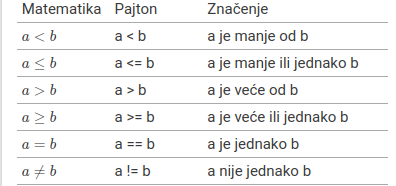
\includegraphics[width=220pt,height=100pt]{slike/operatori_poredjenja.png}
	\caption{Osnovni operatori poređenja u Pajtonu.}
	\label{fig: operatori_poredjenja}
\end{figure}

\subsection{Uslovna naredba If}

Sintaksa bazne naredbe \texttt{if} (sa neobaveznom alternativom) je data sa:
\begin{minted}{python}
    if uslov:
        naredba_1
    else:
        naredba_2
\end{minted}

Tok naredbe je sljedeći: ako je \emph{uslov} ispunjen, izvršava se \textit{naredba\_1} (koja može da bude i blok naredbi), inače se izvršava blok \textit{naredba\_2}. Primijetimo pravila uvlačenja ili indentacije (eng. \textit{indentation}) k\^oda pod \texttt{if} blokom koja se moraju poštovati kao sintaksno pravilo. Nakon izvršavanja jedne od naredbi, program izlazi iz ugnježdenog bloka \texttt{if} naredbe, te prelazi na izvršavanje sljedeće naredbe po redu u programu. Kao i u svakom programskom jeziku, tok izvršavanja naredbi je  odozgo prema dolje. Primijetimo da prethodna sintaksa za \texttt{if} radi sam samo dvije alternative. \texttt{If} koji dozvoljava više alternativa se poziva na sljedeći način. 

 \begin{minted}{python}
 	if uslov_1:
 	   naredba_1
 	elif uslov_2:
 	   naredba_2
 	...
 	elif uslov_k:
 	   naredba_k
 	else:
 	    naredba_n
 \end{minted}

Program provjerava redom uslove krenuvši od prvog. U slučaju da se naiđe na  uslov koji je tačan, izvršavaju se odgovarajuće naredbe (u sklopu ugnježdenog  bloka), te program  nastavlja sa izvršavanjem prve naredne naredbe poslije \texttt{if} naredbe pod istim bloku. U slučaju da niti jedan od uslova nije tačan, izvršava se \emph{naredba\_n} (ulazi u ugniježdeni blok pod \textit{else} komandom). Nakon toga, izlazi se iz \texttt{if} bloka te program nastavlja sa prvom narednom naredbom pod istim blokom (uravnanjem).  

\subsection{For i While petlje }

Petlje se koriste za iterativno izvršavanje bloka k\^oda, sve dok se ne ispuni određeni uslov (prekida). Pajton sadrži dvije vrste petlji: \texttt{for} i \texttt{while} petlja.

Petlja se može koristiti \texttt{for} za iterisanje kroz nizovne objekte (kao što je lista, torka, ili string) ili duge iterabilne objekte (rječnici i skupovi).

Sintaksa za petlju \texttt{for} je data sa:
\begin{minted}{python}
     for item in iterable:
         naredba # blok koda koji se izvršava
\end{minted}
gdje je \emph{item} varijabla kojoj se dodjeljuju elementi iterabilnog objekta \textit{iterable} (lista, torka), jedan po jedan, dok se za svaku takvu dodjelu izvrši blok k\^od \emph{naredba}. 
 
Sintaksa za petlju \texttt{while} je data sa:

\begin{minted}{python}
    while uslov:
	  naredba # blok koda koji se izvršava
\end{minted}
\emph{Uslov} podrazumijeva bulov izraz, koji se provjerava prije svakog izvršavanja blok koda \emph{naredba}, koja se potom izvršava ukoliko izraz \emph{uslov} vraća vrijednost  \emph{True}, inače se izlazi iz petlje i tok izvršavanja programa seli na prvu narednu naredbu u programu na istom nivou ugnježdnja kao i \texttt{while} petlja. 

Npr. ispisivanje prvih 10 parnih cijelih brojeva pomoću \textit{while} petlje se dobija izvršavanjem sljedećeg k\^oda.

\begin{minted}{python}
	i = 1
	while i <= 10:
	    print(2*i)
	    i += 1 # Komentar: ekvivalentno dodjeli i = i + 1
\end{minted}

\section{Složene strukture podataka}

Postoji nekoliko osnovih struktura podataka  u Pajtonu koje su fundamentalne za primjenu i rješavanje problema, a to su: stringovi, liste, rječnici (heš mape), torke i skupovi, između ostalih.  %Svaka od ovih struktura  predstavljaja kolekciju elemenata (objekata). 

\subsection{Stringovni tip podataka}

\texttt{Str} je ugrađeni tip podataka (klasa) koji služi za predstavljanje niza Unicode karaktera. Stringovi u Pajtonu su nepromjenjivi; u prevodu, kada se string kreira, ne može se više mijenjati.

\textit{Inicijalizacija}. Da biste se kreirao string, stavimo niz karaktera u jednostruke (') ili dvostruke navodnike (").

\begin{minted}{python}
	string0 = 'hello'
	string1 = "world"
\end{minted}

Višelinijski stringovi se kreiraju koristeći trostruke navodnike. 

\begin{minted}{python}
	multiline_str2 = '''Ovo je
	višelinijski string.'''
\end{minted}

\textit{Metode}.
\begin{itemize}
	\item Konkatenacija stringova se realizuje pomoću operatora '+'. 
	\item Pristupanje karakterima stringa je obezbjeđeno operatorom '[]'. Karakteri stringova su indeksirani brojevima $0, 1,\ldots$ idući od početka stringa ka njegovom kraju, ili sa $-1, -2,\ldots$ idući sa kraja stringa ka početku  (reverzno). 
	\item Rezanje stringa (eng. \textit{slicing}) se realizuje sa `[:]' na sljedeći način:
	\begin{minted}{python}
	 string1 = 'world'
	 substr1 = string1[1:3] # Output: 'or'
	 substr2 = string1[:3] # Output: 'wor'
	\end{minted}
	
	\item  Binarnim operatorom '*' ``lijepimo'' više istih kopija stringa u jedan novi. Drugim argumentom operatora definišemo broj kopija datog stringa.  
	\item Dužina stringa se dobija primjenom funkcije \emph{len}(). 
	\item Brisanje stringa iz memorije se realizuje pomoću ključne riječi \textit{del} koja se pozicionira ispred stringa koji se briše. 
    \item Postoji mnogo pomoćnih funkcija koje nabrajamo ovdje bez detalja: \textit{lower}(), \textit{upper}(), \textit{strip}(), \textit{replace}(), \textit{find}(), itd. 
\end{itemize}

\textit{Memorijska organizacija}. Objekat tipa \texttt{str} je predstavljen nizom Unicode karaktera koji je smješten u neprekidnom bloku memorije. Svaki karakter u tom nizu je predstavljen brojem (kodom) tog karaktera u Unicode standardu. Svaki takav k\^od je predstavljen fiksnim brojem bajtova, u zavisnosti od platforme, što je obično ili 2 ili 4 bajta. Stringovi se često prosljeđuju kao reference na originalni stringovni objekat. %U prevodu,   ako dvije varijable referenciraju na isti string, promjene koje su napravljene putem jedne varijable vidljive su takođe putem druge varijable.

	\begin{figure}
	\centering
	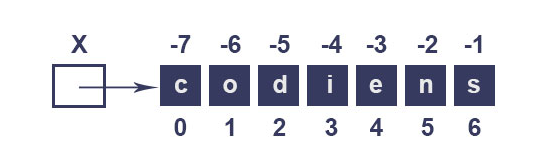
\includegraphics[width=200pt,height=60pt]{slike/str_mem_organization.png}
	\caption{Pojednostavljen prikaz unutrašnje memorijske strukture jednog stringa   u Pajtonu. }
\end{figure}


\textit{Dodatne napomene}. Objekat tipa \texttt{str} u Pajtonu predstavljen je u jeziku \textit{C} kao struktura koja sadrži pokazivač na početak niza podatka (string), kao i druge metapodatke kao što su dužina stringa i trenutna količina dodijeljene memorije za niz.

Definicija odgovarajuće \textit{C} strukture za pajtonov \texttt{str} objekt izgleda ovako:

\begin{minted}{C}
	typedef struct {
		long ob_refcnt;
                PyTypeObject *ob_type;
		Py_hash_t ob_shash;
		Py_UNICODE* st_val
	} PyUnicodeObject;
\end{minted}

Polje ob\_shash se koristi za pohranjivanje keširane vrijednosti niza, a tip Py\_UNICODE se koristi za predstavljanje Unicode znakova u procesu interpretacije programa. %U Pajtonu 3.x, Py\_UNICODE je ekvivalentan ugrađenom tipu \texttt{str} i definisan je kao 2-bajtni ili 4-bajtni neoznačeni cijeli broj.  %u zavinosti od toga kako je Python izgrađen.
 
Jednostavno rečeno, string  pohranjuje  podatke kao neprekidni niz Unicode znakova. %, sa null-terminatorom na kraju. 
Struktura PyUnicodeObject sadrži pokazivač na ove podatke.


Kada se objekt tipa \texttt{str} kreira, prvo se memorija dodjeljuje nizu, a potom se inicijalizuju i metapodaci. Pri nizovnoj manipulaciji, interni bafer se eventualno mijenja kako bi se prilagodio novim podacima. Objekt \texttt{str} je   optimiziran za dijeljenje, kako je već napomenuto. %Preciznije, ako više \texttt{str} objekata sadrži iste znakovne podatke, oni mogu dijeliti isti interni bafer podataka radi uštede memorije. 
 Za stringove je vezan i proces   \textit{interniranja stringova} što označava ponovnu upotrebu postojećih stringovnih objekata umjesto stvaranja novih sa istom vrijednošću. Ovaj proces se izvodi   globalnim keširanjem string objekata i provjerom    keš memorije prije kreiranja novog string objekta. Ako string objekt sa istom vrijednošću već postoji u kešu, on se vraća umjesto kreiranja novog objekta. Ovaj proces štedi memoriju i poboljšava performanse programa, posebno kada se radi sa većim brojem manjih stringovnih objekata.


\subsection{Liste}
Lista je nehomogena, uređena, indeksirana i promjenljiva kolekcija elemenata. U jeziku Pajton se inicijalizuje kao objekat klase \texttt{list}. Elementi ove kolekcije su indeksirani brojevima, krenuvši od 0. Pajton, za razliku od većine programskih jezika, dopušta indeksiranje negativnim brojevima gdje je u tom slučaju indeks posljednjeg elementa liste -1, pretposljednjeg -2, itd.  

\textit{Inicijalizacija}.

\begin{minted}{python}
	 lista = list()
	 lista1 = ["a", "b", 2.0, 3]
	 lista2 = list(("abc", "sef", 2))
\end{minted}

\textit{Osnovne metode}.   

\begin{itemize}
	\item Operator [$index$]: vraća element liste na poziciji \textit{index} (prvi element liste indeksiran sa 0); 
	\item Operator otkidanja \textit{[indeks1 : indeks2 : k]}: vraća listu uzimajući svaki \textit{k}-ti  element date liste  krenuvši sa elementom na poziciji \textit{indeks1} (0 ako nije naveden),  pa sve do elementa sa indeksom \textit{indeks2} (dužina liste, ako nije naveden) isključno; 
	\item Operator \textit{in}: ispituje da li je element u listi -- vraća \emph{True} ili \emph{False};
	\item \texttt{for} $x$ in \emph{lista}: iterisanje kroz listu prema indeksu; 
	\item \textit{append(elem)}: dodaje se element na kraj liste;
	\item  \textit{remove(elem)}: briše element \textit{elem} iz liste;
	\item  \textit{pop}(): briše posljednji element iz liste;
	\item  \textit{insert(index, elem)}: postavlja element \textit{elem} na poziciji \textit{index} u listi;
	\item  \textit{reverse()}: vraća reverznu  listu date liste; 
	\item \textit{copy}(): pravi kopiju elemenata liste u drugu listu. 
 \end{itemize}

\textit{Memorijska organizacija}.  U pajtonu su liste realizovake kao \textit{dinamički} nizovi. To znači da mogu povećavati ili smanjivati veličinu shodno dodavanjem ili brisanjem elemenata, respektivno. Upravljanje memorijom listi se obezbjeđuje interpreterom.  Pri inicijalizaciji liste, jedan blok memorije se određuje za skladištenje njenih elemenata, pogledati Sliku~	\ref{fig: mem_list_org}.  Veličina ovog bloka memorije zavisi od broja elemenata u listi i korištenog pajtonovog  interpretera.  Npr. u interpreteru (CPython)  memorija je unaprijed dodijeljena u komadima (eng. \textit{chunk}).
%https://rushter.com/blog/python-memory-managment/ https://www.opensourceforu.com/2021/05/memory-management-in-lists-and-tuples/

 \begin{figure}[!ht]
	\centering
	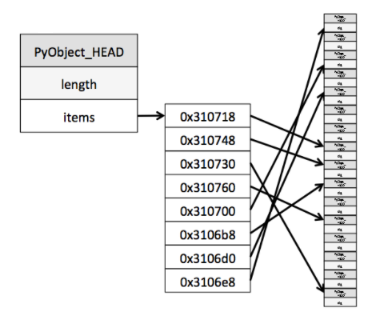
\includegraphics[width=230pt,height=160pt]{slike/list_mem_org.png}

	\caption{Liste u pajtonu: memorijska organizacija} 	\label{fig: mem_list_org}
\end{figure}


\begin{figure}[!ht]
	\centering
	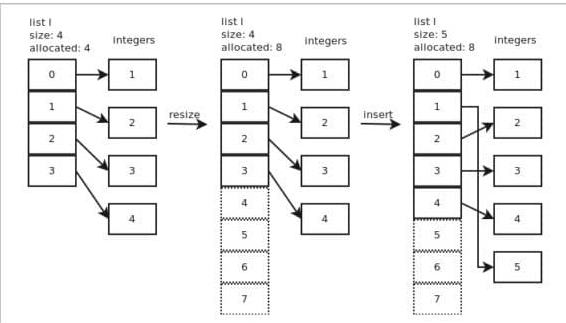
\includegraphics[width=320pt,height=150pt]{slike/list_mem_management.png}
	\caption{Liste u pajtonu (pojednostavljena prezentacija): dodavanje elementa 5 na početnu listu} 
\end{figure}%\footnote{Slika sa linka: \url{https://www.laurentluce.com/images/blog/list/list_insert.png}}


 Kada se lista promijeni, interpreter po potrebi dodijeljuje novi blok memorije veće veličine gdje se postojeći elementi liste kopiraju u novododijeljeni blok. Ovaj proces se naziva \textit{realokacija}.  U slučaju kada je potrebno osigurati čuvanje niza, a realokacija nema toliko prostora, stvoriće se nova memorija i kopija što će rezultirati veoma skupom operacijom. Da bismo se to izbjeglo, možemo unaprijed rezervisati potrebnu memoriju. To se može uraditi sljedećim kodom:
 \begin{minted}{python}
    lista =  [None] * max_broj_elemenata
 \end{minted}

Da bi se elementi liste automatski obrisali od strane pajtonovog sakupljača otpadaka, listi je potrebno dodijeliti \texttt{None} vrijednost.  U tom slučaju, svi elementi liste koji nemaju drugih (aktivnih) pokazivača koji pokazuju na date elemente se automatski brišu iz memorije. 

%https://www.analyticsvidhya.com/blog/2021/05/why-you-should-avoid-using-python-lists/
\textit{Dodatne napomene}. Kao što smo napomeuli, za razliku od nizova u programskom jeziku $C$, liste mogu biti heterogene. Međutim, ova fleksibilnost je prilično skupa. Da bi lista bila heterogena, svaki od elemenata liste mora sadržavati informaciju o vlastitom tipu, broju referenci, stvarnu vrijednost na koju pokazuje itd. Drugim riječima, svaka stavka je kompletan pajtonov objekat. Dakle, ako   dalje raščlanimo, lista u pajtonu sadrži pokazivač koji   pokazuje na   blok pokazivača, a unutar svakog bloka,  pokazivači redom pokazuju na odvojeni (puni) pajtonov objekat.  Ako su sve varijable istog tipa, većina ovih informacija postaje suvišna. Alternativa u takvom slučaju je korištenje \textit{array} ugrađenog tipa, o kojem više govorimo u sljedećem odjeljku.   %poput onog koji smo vidjeli ranije. %% Ovo je kao jedna velika lutka!

\subsection{Nizovi: modul Array}

Pajton sadrži ugrađeni modul \textit{array} koji je sličan nizovima u jeziku  \textit{C} ili \textit{C}++. U ovom kontejneru, podaci se smiještaju u neprekidnom bloku memorije. Kao i nizovi u jeziku \textit{C} ili \textit{C}++, oni podržavaju unos jednog tipa podataka u isto vrijeme, dakle nisu heterogeni poput listi u Pajtonu, već homogene strukture. Indeksiranje je slično listama. Tip eleemnata niza mora biti specificiran pomoću koda, koji su pobrojani u Tabeli~ \ref{tab: Tip podataka u objektu array} (podešavajući vrijednost parametra \textit{typecode}). 

\begin{table}[!ht]
	\centering
	\begin{tabular}{llll}  \hline \hline
		Code      & Datatype                  & Python type & Size (Byte) \\ \hline \hline
		`b' / `B' & signed / unsigned char    & int   & 1 \\
		
		`h' / `H'  & signed / unsigned  short  & int   & 2 \\
        `i' / `I'  & signed / unsigned int     & int   & 2 \\
        `l' / `L'  &  signed / unsigned long   & int   & 4 \\
        `q' / `Q'  & signed / unsigned long long & int & 8 \\
        `f'        & float                       & float & 4 \\
         `F'       & double                      & double & 8 \\ \hline \hline
		
	\end{tabular} 
\caption{ Tip podataka u objektu \textit{array}}\label{tab: Tip podataka u objektu array}
\end{table}

Da bismo koristili modul \texttt{array}, prvo ga uvedemo sa naredbom \texttt{import}: 
\begin{minted}{python}
 import array 
\end{minted}

\textit{Inicijalizacija. } 
\begin{minted}{python}
    my_array =  array('i', [1, 2, 3, 4, 5])
\end{minted}

\textit{Osnovne metode}. 
\begin{itemize}
	\item Pristup svakom elementu se postiže korištenjem uglaste zagrade; indeksiranje elemenata kreće od 0. 
	\begin{minted}{python}
print(my_array[0])  # Output: 1
print(my_array[2])  # Output: 3
	\end{minted}

\item Modifikacija elemenata se vrži pomoću operatora dodjele (kao i u listama):
\begin{minted}{python}
	my_array[0] = 7
	
	print(my_array)  # Output: array('i', [7, 2, 3, 4, 5])
\end{minted}
\item Funkcije \textit{append}(), \textit{extend}(),  \textit{insert}(), \textit{remove}() i \textit{pop}():  imaju istu ulogu kao i odgovarajuće funkcije u listi. Pogledajmo primjer sa \textit{extend}(): 
\begin{minted}{python}
floats = array('f', [2.0, 3.2, 1.4 ])

tuple_floats = (1.1, 4.1, 5.2, 9.0)

floats.extend(tuple_floats) # dodavanje (kolekcije) elemenata
\end{minted} 
  
\end{itemize}

%\textit{Memorijska organizacija}. 

\subsection{Rječnici}
Rječnici su neuređene, promjenljive, i indeksirane kolekcije elemenata koji su dati u obliku para ključ--vrijednost. Za indeksiranje elemenata upravo služi par ključ--vrijednost koji je jedinstven na nivou objekta ove strukture. Često ime za rječnik je heš mapa. Klasa koja podržava kreiranje objekata koji predstavljaju rječnike je \texttt{dict}. 

\textit{Inicijalizacija}.  

\begin{minted}{python}
	# Vitičaste zagrade
	dct = {"ime": "Mirko", "godine": 30, "grad": "Banja Luka"}
	
	# dict() konstruktor
	dct1 = dict(ime="Mirko", godine=30, grad="Banja Luka")
\end{minted}


\textit{Metode}. 
\begin{itemize}
	\item   Pristup vrijednosti odgovarajućeg ključa:
	
	\begin{minted}{python}
 my_dict = {"ime": "Mirko", "age": 30, "grad": "Banja Luka"}
 print(my_dict["ime"])  # Izlaz: Mirko
	\end{minted}
	
     \item Ažuriranje vrijednosti:
     	
     \begin{minted}{python}
my_dict["godine"] = 31
 
     \end{minted}
U slučaju da dati ključ ne postoji u mapi, par  (``godine'', 31) se dodaje u mapu.  Ako ne želimo posljednji scenario dodavanja, koristi se metoda \textit{update()}.
\item Brisanje elementa: koristi se metod pop(\textit{key}) ili ključna riječ \textit{del}:
 \begin{minted}{python}
	dct = {"ime": "Mirko", "godine": 30, "grad": "Banja Luka"}
	del dct["grad"]
	print(dct)  # Output: {"ime": "Mirko", "godine": 30}
	
	dct = {"ime": "Mirko", "godine": 30, "grad": "Banja Luka"}
	dct.pop("grad")
	print(dct)  #  Output: {"ime": "Mirko", "godine": 30}
 
\end{minted}

\item Provjera da li ključ postoji u heš--mapi: koristimo operator \textit{in}:
 \begin{minted}{python}
     print("ime" in dct)  # Output: True
     print("pol" in dct)  # Output: False
 \end{minted}
\item Ostale korisne metode: 
\begin{itemize}
	\item \textit{len(dct)}: vraća broj elemenata rječnika \textit{dct};
	\item \textit{keys()}: vraća ključeve mape;
	\item \textit{values()}: vraća sve vrijednosti koji dolaze u paru sa ključevima mape
	\item \textit{items()}: vraća sve parove (ključ, vrijednost) date mape:
\end{itemize}
 \begin{minted}{python}
   for x, y in dct.items():
      print("Ključ=", x, " vrijednost=", y)
 \end{minted}
\end{itemize}
\textit{Memorijska organizacija rječnika}.  U Pajtonu, rječnici su implementirani preko heš tabela, koje su predstavljene nizom parova ključ--vrijednost, gdje su ključevi jedinstveni na nivou objekta i koriste se za vraćanje odgovarajućih vrijednosti. Proces unosa, brisanja i traženja elemenata u heš tabeli je obično veoma brz, sa očekivanim konstantnim vremenom za svaku od operacija.
	
	Kada se rječnik kreira u Pajtonu, prvo se heš tabela određene veličine  inicijalizuje u memoriji koja skladišti parove ključ--vrednost. Veličina heš tabele je obično veća od broja inicijalno unesenih elemenata, kako bi se spriječilo često (dinamičko) menjanje veličine heš mape.
	
	Svaki ključ u rječniku se preslikava u cjelobrojnu vrijednost koristeći heš funkciju, a potom se dobijeni broj koristi kao indeks u heš tabeli. Ako se dva ključa heširaju istom heš vrijednosti, dolazi do pojave heš kolizija. Heš tabela tu situaciju rješava tako što oba para ključ---vrijednost čuva u istom indeksu, stvarajući povezanu listu parova ključ--vrijednost, pogledati Sliku~\ref{fig: dict_mem_organization}. Da bi se dohvatila vrijednost pridružena ključu, Pajton prvo izračunava heš vrijednost ključa pa ga potom koristi za lociranje indeksa u heš tabeli u kojoj je pohranjen odgovarajući par ključ-vrijednost. Ako je ključ pronađen, vraća se odgovarajuća vrijednost; u suprotnom se javlja greška.  Kada se novi par ključ-vrijednost treba dodati u rečnik, pajton izračunava heš vrijednost ključa kojeg koristi za pronalazak  indeksa u heš tabeli na čiju poziciju treba da bude pohranjen novi par ključ-vrednost. Ako je indeks već zauzet drugim parom ključ/vrijednost, novi par ključ--vrijednost se dodaje u   listu povezanu sa tim indeksom. Ako broj parova ključ--vrijednost u rječniku premašuje određenu granicu, heš tabela može promijeniti svoju dužinu kako bi se smanjila vjerovatnoća pojavljivanja heš kolizija u svrhu poboljšavanja performansi.
	
	Što se tiče heš funkcija, Pajton koristi heš funkciju zvanu \textbf{hash()} za ugrađene tipove kao što su stringovi (\texttt{str}), cijeli brojevi (\texttt{int}) i torke (\texttt{tuple}). Međutim, za prilagođene objekte, može se definisati vlastita heš funkcija implementacijom metode \_\_\textbf{hash}\_\_(). Funkcija \textbf{hash()}  vraća cjelobrojnu vrijednost koja predstavlja heš vrijednost objekta. Objekti koji se upoređuju kao jednaki treba da imaju istu heš vrijednost, radi ispravnog funkcioniranja rječnika. Napomenimo da za stringove i bajtove, Pajton koristi algoritam \textit{MurmurHash3} za hešovanje vrijednosti. Ovaj algoritam je konstruisan tako da uniformno raspoređuje heš vrijednosti minimizirajući broj kolizija. Za korisnički definisane klase, Pajton koristi zadanu \textbf{hash()} funkciju, koja generiše jedinstvenu heš vrijednost za svaku instancu klase na osnovu memorijske adrese pridružena instanci. Međutim, kao što je ranije rečeno, ovo ponašanje se može nadjačati definisanjem vlastite heš metode. 
	
	
	\begin{figure}
		\centering
		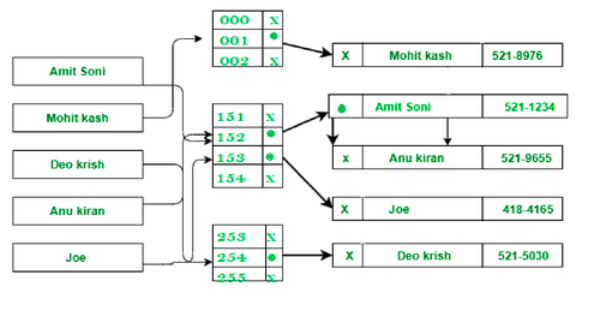
\includegraphics[width=270pt,height=160pt]{slike/dict_mem_organization.png}
 
		\caption{Pojednostavljen prikaz unutrašnje memorijske strukture jedne heš mape (rječnika) u Pajtonu.\footnote{Slika posuđena sa: https://www.geeksforgeeks.org/internal-structure-of-python-dictionary}}		\label{fig: dict_mem_organization}
	\end{figure}
	%https://www.geeksforgeeks.org/internal-structure-of-python-dictionary/ ==> pročitati
	
\subsection{Skupovi}

Skupovi  predstavljaju neindeksirane, neuređene, promjenjive strukture podataka čija je osnovna namjena da se na efikasan način izvrši operacija provjere pripadnosti elementa. Ova struktura odgovara matematičkom pojmu skupa, što znači da duplikati u njoj nisu dozvoljeni. Skup može sadržati bilo koju vrstu elementa kao što je \texttt{int}, \texttt{float}, \texttt{tuple}, \texttt{complex}, itd. ali promjenjive kolekcije kao što su iste, rječnici, skupovi ne mogu biti elementi skupa. 


\textit{Inicijalizacija. }
\begin{minted}{python}
	   skup = set()
	   skup1 = {}  #inicializacija praznog skupa
	   skup2 = set((1, 2, "3"))
	   skup3 = set([1, 2, 3])
\end{minted}

\textit{Osnovne metode}. 

\begin{itemize}
	\item \textit{add(elem)}: dodavanje elementa \texttt{elem} u skup; 
	\item \textit{remove(elem)}: brisanje elementa \textit{elem} iz skupa; izbaciće se greška, ukoliko element ne postoji u skupu (\texttt{KeyError} izuzetak, o izuzecima više u narednim sekcijama);
	\item \textit{discard(elem)}: Uklanja element iz skupa ako je prisutan. Ne aktivira grešku ako element nije u skupu;
	\item \textit{pop()}: Uklanja i vraća proizvoljan element iz skupa;
	\item \textit{clear()}: Uklanja sve elemente iz skupa;
	\item \textit{union()}: Vraća novi skup koji je unija elemenata datog skupa i drugog skupa (koji se prenosi kao vrijednost argumenta metoda); kraći zapis ove metode je pomoću znaka  ``$\mid$''.
    \item \textit{intersection()}: Vraća novi skup koji je presjek datog skupa i drugog skupa; kraći zapis ove metode je pomoću znaka ``$\&$''.
    \item \textit{difference()}: Vraća novi skup koji sadrži razliku između datog skupa i drugog skupa. Kraći zapis ove metode je pomoću znaka ``$-$''. 
\end{itemize}
 
 
 


\textit{Memorijska organizacija}. U Pajtonu se skupovna struktura podataka implementira kao neuređena kolekcija jedinstvenih elemenata. Za implementaciju se koristi heš tabela ili rječnik; elementi skupa su ključevi rječnika dok odgovarajuće vrijednosti njima pridružene nisu od važnosti (mogu se pridružiti \textit{None} vrijednosti, koje se za definisanje nula vrijednosti ili vrijednost koja u suštini  označava ``ništa''. Napomenimo da je \emph{None} vlastiti tip podatka (\texttt{NoneType}).).  

Kada se skupu doda novi element, Pajton uz pomoć odgovarajuće heš funkcije izračunava   heš vrijednost koja odgovara  njegovoj  poziciji u heš tabeli. Ako na dobijenoj poziciji nema elementa, novi element se jednostavno dodaje u skup. U slučaju da već postoji element na toj poziciji, provjerava se da li je novi element jednak postojećem (koristeći metodu \_\_eq\_\_()). Ako su dva elementa jednaka, odbija se dodavanje elementa skupu. Inače, po defaultnom principu se element dodaje u linkovanu listu priduržena datom indeksu. Takođe, određeni kompajleri  
koriste algoritam  otvorenog adresiranja da se pronađe pogodna prazna pozicija u heš tabeli gdje bi se potom dodao novi element. 
Otvoreno adresiranje koristi sekvencijalno ispitivanje pozicija da bi se pronašla prazna pozicija u tabeli. Pozicije se provjeravaju sekvencijalno po nekom pravilu dok se ne pronađe prva prazna. Postoji nekoliko pravila  definisanja sekvence probavanja pozicija, kao što je linearno, kvadratno ispitivanje ili dvostruko heširanje. Npr. ako heš pozicija nije prazna, izračunamo sljedeću poziciju u nizu dodavanjem neke konstantne vrijednosti (recimo 1) trenutnoj heš poziciji kretajući se ciklično po pozicijama heš tabele. Ako je trenutna pozicija 4, a konstantna vrijednost 1, sljedeća pozicija koja se ispituje je 5. Ako je sljedeća pozicija prazna,  element se umeće na tu poziciju. Inače, ponovimo prethodni korak dok god se ne pronađe prazna pozicija ili dok se ne pretraži cijela heš tabela. 
 

Slično, u slučaju kada se element uklanja iz skupa, Pajton prvo izračunava njegovu heš vrijednost pri čemu  pronalazi njegovu poziciju u heš tabeli. Ako postoji element na toj poziciji,  provjerava se da li je jednak elementu koji se želi ukloniti. U slučaju da jeste, element se uklanja iz skupa. %Inače,  koristi se otvoreno adresiranje da traži element u ostatku heš tabele.

Pošto su skupovi implementirani kao heš tabele, prosječna vremenska složenost   skupovnih operacija  dodavanja, uklanjanja i provjere pripadnosti je konstanta, dakle $O(1)$. Međutim, u najgorem slučaju, kada postoji mnogo kolizija u heš tabeli, vremenska složenost može da bude i $O(n)$.

Sljedeći kod pokazuje tip strukture podataka u Pajtonu koja predstavlja skup, a to je upravo ugrađeni tip podataka `set'.

\begin{minted}{python}
		s = {1, 2, 3}
		print(type(s)) # <class 'set'>
\end{minted} 


 	\begin{figure}[!ht]
	\centering
	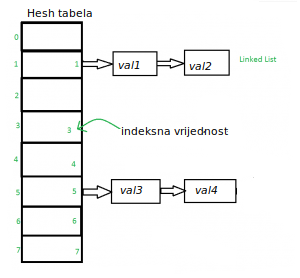
\includegraphics[width=250pt,height=150pt]{slike/set_mem_organization.png}
	\caption{Prikaz unutrašnje memorijske strukture jednog skupa (set) u Pajtonu. }
\end{figure}  %https://www.javatpoint.com/python-set 

\subsection{Torke}
 
 U pajtonu, torka (\texttt{tuple}) je uređena, indeksirana, nepromjenjiva (eng. \textit{immutable}) sekvencijalna kolekcija elemenata, predstavljena jednim objektom u memoriji (na koga pokazuje), dok se ostali objekti određuju implicitnim mehanizmom Pajtona.  Ova struktura dopušta unos duplikata. 
 
 
 \textit{Inicijalizacija}.  
 
 \begin{minted}{python}
 	 my_tuple = ("aa", "bb", 2.0, 3)
 	 my_tuple1 = tuple(["abc", 3.2, 'a'])
 \end{minted}
 
 
 \textit{Osnovne metode}. 
 
 \begin{itemize}
 	\item Pristup elementu torke:
 	\begin{minted}{python}
     my_tuple = (1, 2, 3, 2, 4, 2, 5)
     print(my_tuple[2]) # Output: 3
 	\end{minted}
    \item  Računanje broja pojavljivanja pojedinog elementa:
    
	\begin{minted}{python}    
    my_tuple = (1, 2, 3, 2, 3, 5)
    print(my_tuple.count(2))  # Output: 2
    	\end{minted}
    \item Vraćanje indeksa prvog pojavljivanja elementa u torci:
   	\begin{minted}{python}    
    print(my_tuple.index(2))  # Output: 1
   	\end{minted}
    \item Vraćanje broja elemenata u torci:
       	\begin{minted}{python}    
    	print(len(my_tuple))  # Output: 6
    \end{minted}
    \item Spajanje dvije torke:
  	\begin{minted}{python}    
     my_tuple1 = ("a", "bb", 2)
     my_tuple1 = ("ee", 2, 3.4)
     my_tuple2 = my_tuple + my_tuple1 
     print(my_tuple2) # Output:  ("a", "bb", 2, "ee", 2, 3.4)
    \end{minted}
 \end{itemize}
 
\textit{Memorijska organizacija}.  Pri kreiranju torke, u memoriji se rezerviše fiksna količina memorije za čuvanje svih njenih elemenata. Svaki njen element je pohranjen u kontinuiranom (neprekidnom) bloku memorije, sa fiksnom količinom prostora (nepromjenljiv objekat) dodijeljena svakom elementu na osnovu njegovog tipa.

Memorijska adresa prvog elementa torke se koristi kao referenca na cijeli objekat. U prevodu,  pristup pojedinačnom elementu torke zahtijeva izračunavanje memorijske adrese željenog elementa na osnovu njegovog indeksa i veličine   elemenata u torci. Za posljedicu, pristup pojedinačnim elementima torke se izvršava mnogo efikasnije od pristupa elementima liste jer indeks svakog elementa torke može da se izračuna direktno na osnovu njegove pozicije u memoriji. 

Pošto su objekti tipa \texttt{tuple} nepromjenljive strukture, elementi se ne mijenjaju  nakon što su kreirani. Ako je  potrebno izmijeniti određene elemente, treba da se kreira novi objekat ntorka sa željenim promjenama. Strukture ntorki su  efikasnije u smislu upotrebe memorije u poređenju sa promjenjivim strukturama podataka (liste, rječnici), jer nema potrebe  za dodijelom dodatnih memorijskih lokacija da bismo prilagodili promjene u podacima.
 
 	\begin{figure}
 	\centering
 	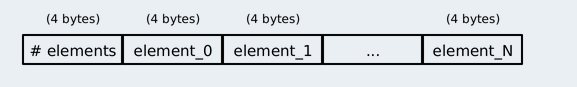
\includegraphics[width=230pt,height=50pt]{slike/tupel_mem_organization.png}
 	\caption{Pojednostavljen prikaz unutrašnje memorijske strukture jednog objekta torke (tuple) u Pajtonu -- \text{element\_0}, \text{element\_1},$\ldots$ predstavljaju pokazivače na vrijednosti  (smješteni na uzastopnim lokacijama). }
 \end{figure}

\section{Funkcije}

Programski jezik Pajton svaku funkciju predstavlja kao jedan objekat. Prema tome, funkcije se mogu dodijeliti varijablama, proslijediti kao argument  drugim funkcijama, a takođe vratiti kao vrijednost    drugih funkcija.  Preciznije, funkcije su implementirane korištenjem Pajtonove interne klase  \texttt{function}. Ova klasa je dio ugrađenih tipova ovog jezika koja pruža osnovnu funkcionalnost za kreiranje i izvršavanje funkcija. Kada se funkcija definiše, interpreter inicijalizuje novi objekat klase \texttt{function} koji predstavlja tu funkciju -- sadrži informacije o nazivu funkcije, argumentima, k\^odu i drugim metapodacima.

Funkcija je predstavljena blokom k\^oda koji obavlja određeni zadatak a može se pozivati i izvršavati više puta kroz program. Uloga funkcija je da se k\^od učini modularnijim, efikasnijim i čitljivijim, jer omogućavaju  podijelu složenih programa na manje dijelove kojima je lakše upravljati.

Sintaksno, funkcije se definišu pomoću ključne riječi \texttt{def} nakon čega slijedi naziv funkcije, zagrade (u kojima se opciono navode argumenti) pa dvotočka. Tijelo funkcije se uvlači ispod zaglavlja. Naredba \texttt{return} vraća rezultat date funkcije, nakon čega se izlazi iz tijela funkcije. Evo primjera jednostavne funkcije koja računa proizvod dva broja:

\begin{minted}{python}
def proizvod_brojeva(x, y):
    prod = x * y
    return prod
\end{minted}

Da bismo pozvali funkciju, koristimo njen naziv nakon čega u zagradama navodimo vrijednosti svih potrebnih argumenata. Npr. da bismo pozvali funkciju iz prethodnog primjera, pišemo sljedeći k\^od:

\begin{minted}{python}
res = proizvod_brojeva(4, 3)
print(res) # Output: 12
\end{minted}

Funkcije mogu imati defaultne vrijednosti dodijeljene parametarima, koje se koriste ako se funkcija pozove bez specificiranja vrijednosti tim parametrima.  Pogledajmo sljedeći primjer 
\begin{minted}{python}
def umnozi(ime="Mirko", umnozi_puta = 1):
    umnozeno = ime * umnozi_puta
    print(umnozeno)
\end{minted}
Ako se prethodna funkcija pozove bez   vrijednosti argumenata, defaultne vrijednosti se prosljeđuju parametrima (vrijednosti ``Mirko'' i 1, redom), a ispisuje se poruka ``Mirko''. 

Dodatno, funkcije mogu imati i opcione parametre, koji su specificirani pomoću operatora zvjezdice (*) ili dvostruke zvjezdice (**). Sljedeći primjer pokazuje upotrebu ovih operatora:
\begin{minted}{python}
def print_brojevi(*nums):
    for num in nums:
    print(num)
def print_vrijednosti_dict(**key_vals):
    for key, vals in key_vals.items():
         print("Ključevi: ", key, " vrijednosti: ", vals)    

print_vrijednosti_dict({"ime": "Mirko", "prezime": "Mirkovic"})
\end{minted}

Funkcije takođe mogu da vraćaju nekoliko vrijednosti koristeći torke:

\begin{minted}{python}
def visestruko_vracanje(x, y):
    dio = x / y
    ostatak = x % y
    return dio, ostatak

d, o = visestruko_vracanje(10, 3)
print(d, " ", o) # Output: 3 1
\end{minted}

%prenos vrijednosti argumenata:

U jeziku Pajton, vrijednosti argumenata funkcije se prosljeđuju referencom objekta. Dakle, kada se funkcija pozove sa svojim argumentom, referenca na objekt se prosljeđuje funkciji, a ne kopija samog objekta. %Jedino objekti koji su nepomjenljivi (kao što su torke) se proslijeđuju funkciji po vrijednosti (kao ``prava'' kopija a ne originalan objekat). 

Ovo može dovesti do   neočekivanog ponašanja u odnosu na neke druge programske jezike, posebno u radu promjenjivim objektima kao što su liste, rječnici i skupovi. Pogledajmo sljedeći primjer:

\begin{minted}{python}
def dodaj_elem_u_listu(elem, lista):

    lista.append(elem)

lista = list(range(1, 4))
dodaj_elem_u_listu(5, lista)
print(lista)  # Output: [1, 2, 3, 5]
  \end{minted}

Kada se pozove funkcija \texttt{dodaj\_elem\_u\_listu} sa vrijednostima 5 i lista, funkciji prosljeđujemo referencu na objekat lista. Izvršavanjem funkcije, mijenja  se lista dodavanjem novog elementa 5.  U slučaju da ne želimo da funkcija modifikuje (promjenljivi) objekt, treba da se napraviti kopija objekta prije njegovog proslijeđivanja funkciji. Više o kopiranju objekata liste će biti riječi u narednim sekcijama.


Nepromjenjivi objekti kao što su cijeli brojevi, decimalni, stringovi i torke se isto prosljeđuju referencom objekta. Međutim, kako su nepromjenjivi, dakle ne mogu se mijenjati, to znači da sve promjene koje radimo na njima unutar funkcije automatski stvaraju novi objekat (na lokalnom steku).

\begin{minted}{python}
def inkrementiraj(x):
    x += 1
    print("Unutar funkcije:", x)

y = 5
inkrementiraj(y) # Output: 6
print(y) # Output: 5
  \end{minted}
Dakle, varijabla $x$ unutar metoda referiše na novi objekat (i nema veze sa proslijeđenim objektom, osim što su istog naziva). Prema tome, iako se nepromjenljivi objekti takođe prenose  putem reference na objekat, bilo kakvo djelovanje funkcije  neće izmijeniti originalni objekat.  Napomenimo da pomoću ključne riječi \textit{global} ispred naziva varijable možemo preinačiti lokalno ponašanje varijable (koja dozvoljava pristup čitanju sadržaja u funkciji) u globalno (gdje je dozvoljeno i pisanje -- mijenjanje sadržaja na koji varaijabla referencira).  

\begin{minted}{python}
def my_func():
    global x
    x = 10
    print(" Vrijednost unutar funkcije :", x)
x = 20
my_func()
print(x) # Output: 10
\end{minted}

Kao što smo napomenuli, funkcija je jedan objekat te se ona može proslijediti kao vrijednost argumentu druge funkcije, kako je to prikazano sljedećim primjerom
\begin{minted}{python}

def dodaj(a, b):
    return a + b
def primjena(func, x, y):
    return func(x, y)

result = primjena(dodaj, 2, 3)
print(result)  # Output: 5
  \end{minted}

\textit{Anonimne funkcije.}  Anonimne funkcije su definirane pomoću ključne riječi \texttt{lambda}, tako da se ponekad nazivaju i lambda funkcije.  Naziv anonimne funkcije su dobile jer ne zahtjevaju eksplicitnu dodjelu naziva kao u regularnoj funkciji. Sintaksa lambda funkcije je data sa:

\begin{minted}{python}
lambda argumenti: izraz
\end{minted}
Pod \textit{argumenti} se podrazumijevaju argumenti funkcije, a \textit{izraz} predstavlja operaciju koja se izvršava nad ulaznim parametrima. Funkcija vraća rezultat koji se dobija izvršavanjem tog izraza uvrštavajući vrijednosti proslijeđenih argumenata. 

Sljedeći primjer daje lambda funkciju za operaciju sabiranja.
\begin{minted}{python}
suma = lambda x, y: x + y
print(suma(4, 3)) # Output: 7
\end{minted}

Ovdje je lambda funkcija pridružena varijabli \textit{suma}, što je moguće jer je svaka funkcija u programskom jeziku Pajton objekat. Potom su ovoj funkciji proslijeđene reference (na vrijednosti 4 i 3). 

Lambda funkcije su često korisne u situaciji kada je potrebno definisati jednostavne (i sadržinski male) funkcije ukoje se koriste u kraćem periodu pa nema smisla da se definišu kao funkcije punog imena. Pored toga, lambda funkcije su često korištene u kombinaciji sa funkcijama, koje su opštepoznate iz funkcijskih jezika, kao što su: \textit{map}(), \textit{filter}(), \textit{reduce}(), o kojima će biti više riječi u nastavku ove knjige, konkretno u Sekciji~\ref{sec:concepts-pyhton}. 


\section{Kompajliranje i izvršavanje programa}

\subsection{Stek vs. Hip} 


Prilikom izvođenja programa, računarska memorija se dijeli na različite dijelove. Dva važna memorijska dijela su stek i hip memorija. 

%K\^od sekcija pohranjuje instrukcije koda u obliku koji mašina razumije. Mašina slijedi upute u sekciji koda. Shodno instrukcijama, 
Pajton interpreter učitava funkcije i lokalne varijable (reference) u memoriju steka. 
Stek memorija je statična i privremena. Statična znači da se veličina objekata pohranjenih u steku ne može da bude promijenjena. Riječ privremeno znači da čim pozvana funkcija vrati svoju vrijednost, funkcija i   varijable vezane za funkciju se uklanjaju sa steka. Pristup memoriji steka nije direktno obezbjeđen programeru, već  briga o ovom dijelu memorije je dodijeljena Pajton interpreteru i OS-u.  Količina memorije koja  se dodijeljuje je poznata interpreteru i kad god se pozove funkcija, njene varijable zauzimaju memoriju koja se rezerviše na steku.
% Pratimo: https://towardsdatascience.com/python-memory-and-objects-e7bec4a2845ž
% O steku i hipu: https://www.geeksforgeeks.org/how-are-variables-stored-in-python-stack-or-heap/

\begin{minted}{python}
	def func():
	
	    # Ove varijable dobijaju memoriju 
	    # alociranu na steku 
	    a = 10
	    b = []
            c = "abc"
\end{minted}

Kao što smo prethodno rekli, varijable (ili reference generalno) skladište samo memorijske adrese objekata. Dakle, postavlja se pitanje gdje se skladište sami objekti? Oni se nalaze u drugoj memoriji koja se zove \textit{hip} (eng. \textit{Heap memory}). Napomenimo da riječ hip nema veze sa istoimenom strukturom podataka  već  zbog dostupnosti gomile memorijskog prostora u svrhu pohranjivanja i brisanja objekata.   Za pohranjivanje objekata potrebna nam je memorija sa dinamičkom alokacijom  -- veličina memorije i objekata se mogu mijenjati. Pajton interpreter je zadužen za aktivno dodeljivanje memorije hipu (Primijetimo da u jeziku $C/C$++ to  se izvršava od strane programera!). Varijable koje su pohranjene u memoriji hipa su: ($i$)   izvan poziva metoda ili funkcija ili ($ii$) dijele se unutar više funkcija, dakle globalnog svojstva.

\begin{minted}{python}
     # Memorija za 10 brojeva
     # je alocirana na hipu
     a = [0]*10     
\end{minted}


Napomenimo još jednom da Pajton koristi algoritam za sakupljanje otpadaka (eng. \textit{garbage collector}) koji održava memoriju hipa čistom, periodično uklanjajući  objekte koji više nisu potrebni.





\subsection{Kompajliranje i izvršavanje}

Proces kompilacije   i izvršavanja k\^oda u programskom jeziku Pajton uključuje sljedeće korake:

\begin{itemize}
	\item \textit{Leksička analiza} -- Izvorni k\^od se prvo prosljeđuje leksičkom analizatoru,  koji razlaže k\^od na pojedinačne tokene kao što su ključne riječi, identifikatori, operatori, itd.
	\item \textit{Parisiranje} -- Tokeni se zatim prosleđuju parseru, koji koristi gramatiku bez konteksta za izgradnju \emph{apstraktnog sintaksnog stabla} (AST) koje predstavlja strukturu k\^oda. U detalje ovog procesa nećemo ulaziti jer izlazi iz domena ove knjige.
	\item \textit{Kompilacija} -- AST se kompajlira u bajtkod, koji je jezik nižeg nivoa,   nezavisan od platforme.  Ovaj bajtkod se čuva u .\textit{pyc} fajlovima kojeg izvršava   pajtonova virtuelna mašina (VM).
	\item \textit{Izvođenje} -- Pajtonova VM izvršava dobijeni bajtkod tako što ga interpretira generišući mašinske instrukcije u hodu. Bajtkod se izvršava u zaštićenom okruženju virtuelne mašine (obezbjeđuje sigurnost i izolaciju od osnovnog OS-a).  
	
\end{itemize}
Napomenimo da tokom procesa izvršavanja, interpreter izvodi nekoliko optimizacija u kodu (npr. eliminaciju repne rekurzije), što može poboljšati performanse k\^oda.
%https://www.geeksforgeeks.org/what-makes-python-a-slow-language/
\begin{figure}[H]	
	\centering
	
	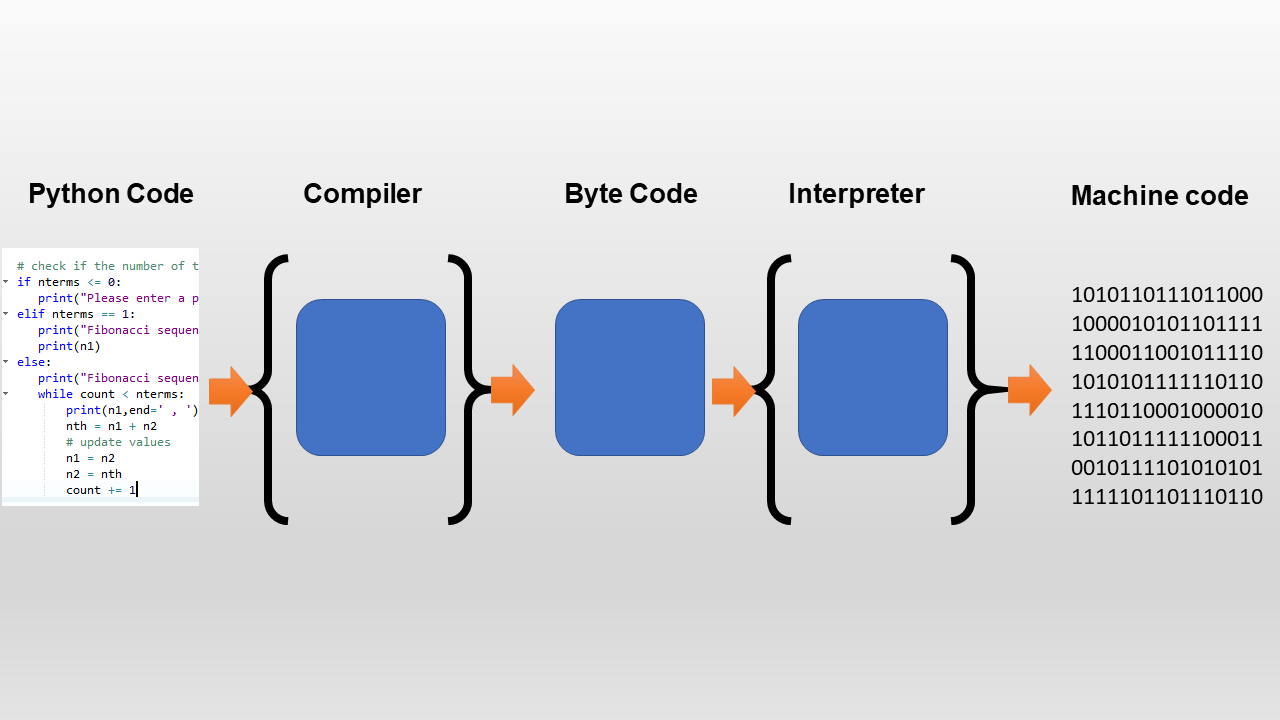
\includegraphics[width=350pt,height=170pt]{slike/python-code-copiler-machine-code.png}%compile_python.png}
\caption{Vizuelizacija procesa izvršavanja pajton koda.}
\label{fig:comp_interpreting}
\end{figure}

%%https://www.astateofdata.com/python-programming/can-python-be-compiled/
% Na osnovu prethodnog, pajton je i kompajliran i interpretiran jezik. 
%https://www.astateofdata.com/python-programming/can-python-be-compiled/ ==> procitati ovdje...

Recimo sada malo više o pajtonovoj virtuelnoj mašini (PVM), bazičnoj komponenti ovog programskog jezika. Kako smo naveli, PVM je odgovorna za interpretiranje bajtkoda i izvršavanje k\^oda. Bajtkod se generiše od strane pajtonovog kompajlera (npr. CPython, Brython) pri kompajliranju izvornog k\^oda.

Ključne uloge PVM su navedene u nastavku. 
\begin{itemize}
\item \textit{Kompatibilnost između platformi}: PVM omogućava izvršavanje pajtonovog k\^oda na više različitih platformi bez ponovne kompilacije. Ovo olakšava pisanje i distribuciju aplikacija.
\item \textit{Poboljšane performanse izvršavanja}: PVM koristi bajtkod  interpreter, koji je brži od direktnog interpretera izvornog k\^oda. PVM može koristiti \textit{Just-In-Time} (JIT) kompilaciju za dalje poboljšanje performansi.
\item \textit{Dinamičko tipiziranje}: Pajton je dinamički tipiziran jezik, što znači da se tip varijable dodjeljuje u vremenu izvođenja programa. PVM je dizajnirana da efikasno upravlja ovim procesom.
\item  \textit{Upravljanje memorijom}: PVM automatski upravlja memorijom, što može olakšati pisanje sigurnog memorijskog k\^oda. PVM  automatski oslobađa memoriju koja se više ne koristi.
\item \textit{Lak pristup eksternim bibliotekama}: PVM se intenzivno koristi u pajton ekosistemu, koji uključuje veliki broj otvorenih biblioteka. Ove biblioteke pružaju širok spektar funkcionalnosti vezano za  veb programiranje, mašinsko učenje, itd. Importovanje boblioteka se vrši pomoću naredbe \texttt{import}. 
\end{itemize}


Na osnovu izloženog, Pajton je i kompajliran (prevodi se u bajtni k\^od) i interpretiran jezik. 
Vizuelizaciju procesa prevođenja programa možete da vidite na Slici~\ref{fig:comp_interpreting}.


\section{O nekim programskim konceptima i ugrađenim funkcijama} \label{sec:concepts-pyhton}

U ovoj sekciji ćemo demonstrirati rad sa nekoliko bitnih i često korištenih ugrađenih funkcija koje su dio standardne pajton biblioteke. Dodatno, biće objašnjen i koncept komprehenzije liste (eng. \textit{list comprehension}) koji  doprinoi modularnosti k\^oda i približava ga konceptima funkcijskih programskih jezika (kao što je Haskel). 

\subsection{Komprehenzija liste}

Komplehenzija liste predstavlja koncizan način za kreiranje liste. To je konstrukcija koja omogućava kreiranje liste u jednoj liniji k\^oda, umjesto da se koriste petlje (i odgovarajuće metode) za iterativnu konstrukciju liste.

Osnovna sintaksa ovog koncepta je sljedeća:

\begin{minted}{python}
	lista = [expr  for item in iterable]
\end{minted}
Ovdje \textit{expr} označava izraz koji se izračunava do vrijednosti koja se smiješta u listu.
Dalje, \textit{item} je varijabla koja  uzima vrijednosti iz (iterabilnog) objekta \textit{iterable}.  Rezultat primjene je nova lista sastavljena od  vrijednosti dobivenih primjenom izraza  \textit{expr} na svaki elemenat objekta \textit{iterable}.

Npr.\ recimo da želimo kreirati listu prvih 10 parnih brojeva. K\^od bi mogao da ide ovako:

\begin{minted}{python}
	parni = []
	for i in range(1, 11):
	    parni.append(2*i)
\end{minted}

Kraći zapis koda, pomoću komprehenzije liste, izgleda ovako:


\begin{minted}{python}
	parni = [2*i for i in range(1, 11)]
\end{minted}
Takođe se  uslovni izrazi  mogu uključiti u koncept komprehenzije liste. Sintaksa je sljedeća:

\begin{minted}{python}
	lista = [expr  for item in iterable if uslov]
\end{minted}
U ovom slučaju, uslovna komanda se odnosi na elemente koje uzima varijabla \textit{item} -- to su samo oni koji zadovoljavaju \textit{uslov}. 

\subsection{Funkcije map, filter, reduce}

Funckije \textit{map}(), \textit{filter}() i \textit{reduce}() su ugrađene funkcije koje se opštepoznate u funkcijskom programiranju. One su korisne kao alati za obradu podataka, posebno kada se radi o velikim skupovima podataka.

Funkcija \textit{map}() uzima dva argumenta: funkciju i iterabilni objekat. Primjenjuje funkciju  na svaki element iterabilnog objekta i vraća iterator na nove elemente kao rezultat. 

\begin{minted}{python}
     brojevi = [1, 2, 3, 4, 5]
     doubled = map(lambda x: x*2, brojevi)
     print(list(doubled))  # Output: [2, 4, 6, 8, 10]
\end{minted}


Funkcija \textit{filter}() uzima dva argumenta: funkciju koja vraća logičku vrijednost i iterabilni objekat. Primjenjuje funkciju na svaki element iterabilnog objekta i vraća iterator na one elemenate za koje je funkcija vratila \emph{True}. 
\begin{minted}{python}
	brojevi = [1, 2, 3, 4, 5]
	parni = filter(lambda x: x % 2 == 0, brojevi)
\end{minted}

Funkcija  \textit{reduce}(): Sintaksa ove funkcije je

\begin{minted}{python}
	reduce(func, iterable[, initial ])
\end{minted}

Ona uzima dva (obavezna) argumenta,  funkciju i iterabilni objekat, te opciono \textit{initial}. Inicijalno, funkcija \textit{func} se primjenjuje na element \emph{initial} i prvi elemenat iterabilnog objekta, te vraća rezultat. Potom,    primjenjuje istu funkciju na vraćeni rezultat i sljedeći element, i tako dalje, sve dok se svi elementi \emph{iterable} objekta ne obrade. 

Pogledajmo sljedeći primjer: 
\begin{minted}{python}
from functools import reduce

numbers = [1, 2, 3, 4, 5]
product = reduce(lambda x, y: x * y, numbers)
\end{minted}

Ovo će primijeniti funkciju množenja na prva dva elementa liste, zatim na rezultat i sljedeći element, i tako dalje, sve dok se svi elementi ne obrade, što rezultira proizvodom svih brojeva liste. Pirmijetimo da funkcija \textit{reduce}() nije dio standardnog pajtonovog modula, već se mora uključiti direktno pozivom \texttt{functools} modula. Više o modulima i radu sa njima ćemo govoriti u narednim sekcijama.



\subsection{Funkcije zip, enumerate i sort}
Funkcije  \textit{zip}() i \textit{enumerate}() su ugrađene funkcije korisne za obradu i iterisanje preko lista ili drugih iterabilnih objekata.

Funckija \textit{zip}() uzima jedan ili više iterable objekata i vraća iterator koji generiše torke koje sadrže uparene elemente svakog iterabilnog objekta (prvi elementi svih listi u jednu torku, drugi elementi svih listi u novu torku, itd.). Sintaksa funkcije je:
\begin{minted}{python}
zip(iterable1, iterable2, ...)
\end{minted}
gdje su \emph{iterable1}, \emph{iterable2},... iterablini objekti. 

Npr. ako imamo dvije liste brojeva i želite da uparite odgovarajuće elemente, imamo sljedeći kod:
\begin{minted}{python}
list1 = [1, 2, 3, 4]
list2 = [5, 6, 7, 8]
parovi = zip(list1, list2) 
print(list(parovi)) # Output: (1, 5), (2, 6), (3, 7),  (4, 8).
\end{minted}
Funkcija \textit{enumerate}() uzima iterativni objekat i vraća iterator koji generiše parove koji sadrže indeks svakog elementa i samog elementa. Sintaksa funkcije je:
\begin{minted}{python}
	enumerate(iterable, start=0)
\end{minted}
gdje je \textit{iterable} jedan iterabilni objekat, a \textit{start} je početna vrijednost indeksa (podrazumijeva se 0). Pogledajmo sljedeći primjer. 

\begin{minted}{python}
voce = ['jabuka', 'banana', 'kruska', 'breskva']
for i, vocka in enumerate(voce):
    print(i, vocka) # (0, 'jabuka'), (1, 'banana'), (2, 'kruska'), (3, 'breskva')
\end{minted}

Funkcija \textit{sort}() je ugrađena funkcija koja se koristi za sortiranje elemenata   liste po nekom kriterijumu. Ona je metoda liste koja ne vraća ništa već je njen zadatak sortirati listu (u memoriji koja je već dodijeljena).

Sintaksa ove funkcije data je u nastavku 
\begin{minted}{python}
	sort(reverse=False, key=None)
\end{minted}

Argument \textit{reverse} prosljećuje poredak sortiranja u listi na način da ukoliko mu je dodijeljena vrijednost \emph{True}, lista će biti sortirana u opadajućem, a inače (po defaultu) redoslijed sortiranja je rastući. Kriterijum sortiranja (kao funkcija) se proslijeđuje argumentu funkcije \textit{key}. Primijetimo da ukoliko se kriterijum sortiranja ne proslijedi eksplicitno, Pajton koristi interne relacije poretka za tip objekata, ukoliko su oni uporedivi (predefinisanom relacijom totalnog uređenja, kao kod osnovnih tipova podataka). U slučaju da objekti nisu uporedivi, vraća se poruka o greški.  Jedna od mogućih grešaka koja se može javiti je sljedeća:
\begin{minted}{python}
TypeError: '<' not supported between instances of 'str' and 'int'
\end{minted}


Primjer sortiranja numeričkih vrijednosti je dat k\^odom:
\begin{minted}{python}
brojevi = [6, 3, 8, 3, 1, 7]
brojevi.sort(reverse=True)
print(brojevi) # Output: [8, 7, 6, 3, 3, 1]
\end{minted}
  Takođe je moguće koristiti funkciju \textit{sorted}() za sortiranje liste i vraćanje nove sortirane liste bez mijenjanja originalne liste:
\begin{minted}{python}
brojevi = [5, 2, 8, 3, 1, 7]
sort_brojevi = sorted(brojevi)
print(sort_brojevi)
\end{minted}

Postoji i niz drugih pomoćnih funkcija od opšte koristi, koje ćemo pobrojati u nastavku bez ulaska u detalje o njihovoj sintaksi i korišćenju:
\begin{itemize}
	\item \textit{sum}(iterable): vraća sumu vrijednosti elemenata iterabilnog objekta \emph{iterable};
	\item \textit{eval}(expr): vraća vrijednost izraza \emph{expr} zapisan u stringovnom zapisu;
	\item \textit{round}(num, dec\_place): zaokruživanje decimalnog broja na proslijeđen broj decimala;
	\item \textit{max}(iter): vraća broj maksimalne vrijednosti među proslijeđenim brojevima;
	\item \textit{abs}(num): vraća apsolutni vrijednost broja. 
\end{itemize}
\section{Uopšteno o modulima}

\textit{Modul} je datoteka koja sadrži Pajtonove definicije i naredbe. Naziv datoteke je naziv modula sa sufiksom .\textit{py}.

Modul može sadržati različite definicije kao što su funkcije, klase i varijable, koje se mogu uvesti i koristiti u drugim Python skriptama ili modulima. To olakšava organiziranje i ponovnu upotrebu k\^oda u različitim projektima.

Da bismo koristili modul u Pajtonu, prvo ga mora uvesti pomoću naredbe \texttt{import}. Npr. ako imamo modul pod nazivom \textit{mojmodul}.py, možemo ga uvesti na sljedeći način:
\begin{minted}{python}
	import mojmodul
\end{minted}


Nakon što smo uvezli modul, možemo pristupiti njegovim funkcijama, klasama i varijablama pomoću notacije tačka. Npr. ako \textit{mojmodul} sadrži funkciju pod nazivom \texttt{mojafunkcija}, poziva se ovako:
\begin{minted}{python}
mojmodul.mojafunkcija()
\end{minted}

Takođe se može koristiti i ključna riječ \texttt{from} za uvoz određenih funkcija ili klasa iz modula:
\begin{minted}{python}
from mojmodul import mojafunkcija
\end{minted}

Ovo će omogućiti direktno korištenje funkcije bez potrebe za tačaka notacijom:

\begin{minted}{python}
mojafunkcija()

\end{minted}

Pajton dolazi s velikim brojem ugrađenih modula, među kojima izdvajamo \texttt{math}, \texttt{random}, \texttt{datetime}, \texttt{os} i \texttt{numpy} o kojima će biti riječi u nastavku ove sekcije. Ovi moduli se uključuju direktno sa instalacijom jezika Pajton.
 
%Napomenimo da se mogu kreirati i vlastite module koji prvenstveno služe da bolje organizovanje i reiskorištavanje vlastitog koda.

\subsection{Instaliranje eksternih modula} 


Da bismo instalirali eksterne module u Pajtonu,   koristi se menadžer paketa \textit{pip}, koji je direktno uključen u većinu instalacija pajtona. 

Koraci za instaliranje eksternih modula pomoću \emph{pip}-a su dati u nastavku. Otvorimo terminalnu konzolu i upišemo naredbu \textit{pip install naziv\_modula}, gdje je \textit{naziv\_modula} (obično) odgovara nazivu  modula kojeg želimo instalirati. Npr. da bismo instalirali modul \textit{requests}, pišemo:
\begin{minted}{python}
    pip install requests
\end{minted}

Pritiskom enter tastera, instalacija se pokreće; pip automatski preuzima modul iz PyPI (eng. \textit{Python Package Index}) i instalirati ga u trenutno pajton okruženje. PyPI je veliki repozitorij softverskih paketa koji su napisani u pajtonu, besplatno dostupni za korištenje. Sadrži više od 300,000 paketa koje možemo instalirati pomoću \textit{pip} menadžera.


Kada proces instalacije modula uspješno završi, on se interno može koristiti pomoću naredbe \textit{import}. Npr. da bismo koristili modul \textit{requests}, pišemo sljedeće:
\begin{minted}{python}
    import requests
\end{minted}
Takođe se možete navesti određena verziju modula za instalaciju dodavanjem  ``==''  iza kojeg slijedi broj verzije nazivu modula. Npr. da bismo instalirali verziju 2.2.1 modula \textit{requests},  pisali bismo:
\begin{minted}{python}
pip install requests==2.2.1
\end{minted}


\subsection{Modul Math}

\texttt{Math} je matematički modul koji za rad nudi različite matematičke funkcije i konstante. Da bismo koristili matematički modul u svom programu, prvo morate uvesti pomoću naredbe \textit{import math}.

Nakon štose uveze matematički modul, omogućeno je korištenje njegovih funkcija i konstanti u k\^odu. Navedimo nekoliko konkretnih primjera. 

\begin{minted}{python}
import math

# Računajmo korjen broja
x = math.sqrt(25)
print(x)  # Output: 5.0

# Konstanta Pi
pi = math.pi
print(pi)  # Output: 3.141592653589793

# Računanje sin 
sin_angle = math.sin(45)
print(sin_angle)  # Output: 0.7071067811865475
\end{minted}

Neke od češće korištenih metoda ovog modula su:   \textit{sqrt}(), \textit{pow}(), \textit{log}(), \textit{exp}(), \textit{log10}(), \textit{floor}(), \textit{ceil}(), \textit{fabs}(), \textit{gcd}(), \textit{dist}() – Euklidova udaljenost između dvije tacake (predstavljene kao torke, ili liste), \textit{isnan}(), \textit{sin}(), \textit{cos}(), \textit{tan}(), \textit{sinh}(), \textit{asin}(), među ostalim metodama.

U nastavku navodimo jednu od internih implementacija korjene funkcije \textit{sqrt}() broja $x\geq 0$. Ona je implementirana  korištenjem algoritma koji se zove \textit{Babilonova metoda}, poznata i pod nazivom Heronova metoda. Algoritam je numerička iterativna metoda koja aproksimira kvadratni korijen broja \textit{x} uzimajući prosjek prethodne aproksimacije i vrijednosti količnika broja $x$ i vrijednosti dobijene u prethodnoj aproksimaciji. Proces se nastavlja sve dok aproksimacija nije dovoljno precizna. Preciznije, primjeljuje se naredna rekurzija:
\begin{center}
	$y_{n+1}= \frac{1}{2}(y_n + \frac{x}{y_n})$
\end{center}
za neki proizvoljan inicijalni korak $y_0> 0$. Trivijalno, za $x=0$, vraća se vrijednost 0. Algoritam se izvršava dok se ne postigne unaprijed zadana preciznost $\epsilon$ broja $x$, tj. dok ne bude ispunjeno $|y_{n+1} - \frac{x}{y_n}| \leq \epsilon$. 
\subsection{Modul Random}

Modul \texttt{random}  pruža skup funkcija za generiranje (pseudo-)slučajnih brojeva,   korisni u različitim aplikacijama kao što su  kriptografija i razvoj igara.

Navedimo neke osnovne funkcije ovog modula.

\begin{itemize}
	\item   \textit{random}():  slučajan nasumični \textit{float} broj između 0 i 1, uključujući 0, ali isključujući 1;
	\item \textit{randint}(\emph{a, b}):  generiše nasumični cijeli broj između $a$ i $b$, uključujući oba broja,  $a$ i $b$.
	\item  \textit{choice}(\emph{seq}):  vraća slučajan element datog niza \textit{seq}; 
	\item \textit{shuffle}(\emph{seq}): nasumično permutuje elemente u datom nizu \textit{seq};
	\item \textit{sample}(\emph{populacija, k}): Ova funkcija vraća nasumično odabran uzorak od $k$ elemenata iz date populacije  \textit{populacija} bez zamjene;
	\item \textit{seed}($a$=None): inicijalizuje generator slučajnih brojeva. Ako argument \textit{a} nije naveden, koristi se sistemsko vrijeme.
 
\end{itemize}

Implementacija funkcije \textit{random}() u Pajtonu koristi algoritam generatora pseudo-slučajnih brojeva, koji je deterministički a generiše niz brojeva koji se čini slučajnim. Algoritam koji se koristi u funkciji \textit{random}() je algoritam \textit{Mersenne Twister},  široko korišten   za generiranje pseudo-slučajnih brojeva.

Algoritam \textit{Mersenne Twister} generiše niz 32-bitnih cijelih brojeva koristeći specijalni linearni pomaknuti (eng. \textit{shift})  registar povratne sprege,  koji koristi operacije isključivanja ili (XOR) za generiranje izlaza. Algoritam koristi veliki prost broj koji se zove \textit{Mersenov} prost ($2^{19937}-1$) kao modul, koji osigurava da generisani niz ima dug period   i dobra statistička svojstva. Inače, algoritam su razvili Makoto Matsumoto i Takuji Nishimura 1997. godine. Drugi generator  koji se može koristi je prosti \textit{linerarni kongruentni generator} 
koji generiše  slučajne brojeve po rekurziji
$$ x_{n+1} = (a x_n + b)\ \%\ m $$
gdje je $x_0$ početni sid vrijednosti između 0 i $m-1$. 

\subsection{Modul Time}

Modul  \texttt{time} je ugrađeni modul koji pruža razne funkcije povezane sa radom sa vremenom. Omogućuje   izvođenje raznih operacija, kao što su vraćanje trenutnog vremena, uspavljivanje procesa na određeno vrijeme,  pretvaranje formata vremena i još mnogo toga.

U nastavku navodimo najčešće korištene funkcije koje pruža ovaj modul:
\begin{itemize}
	\item  \textit{time}(): Vraća trenutno vrijeme u sekundama od epohe (eng. epoch) (računa se kao datum 01.01.1970) kao float tip. 
	\item time.\textit{sleep}(\textit{secs}): obustavlja izvršenje trenutne n\^iti na zadani broj sekundi \textit{secs}. 
	\item time.\textit{localtime}([\textit{secs}]): Pretvara vrijeme u sekundama \textit{secs} od epohe u torku koja predstavlja lokalno vrijeme u obliku:  godina, mjesec, dan, sat, minuta, sekunda, radni dan, Julijanski dan, DST.
\end{itemize}


\subsection{Modul Os}

\texttt{Os} modul je ugrađeni  modul koji pruža mogućnost korištenja funkcionalnosti zavisne od operativnog sistema kao što je čitanje ili pisanje u sistem datoteka, upravljanje procesima, varijablama okruženja i mnogi drugim sistemskim zadacima.

Nekih od najčešće korištenih funkcija koje pruža ovaj modul su:

\begin{itemize}
	\item os.name: Vraća naziv operativnog sistema (npr. `posix' za Linux i macOS, `nt' za Windows).
	\item  \textit{getcwd}(): Vraća trenutni radni direktorij kao u obliku stringa.
	\item  \textit{chdir}(\emph{path}): Mijenja trenutni radni direktorij na specificiranu stazu \emph{path}.
	\item \textit{listdir}(\emph{path}): Vraća listu datoteka i direktorija u navedenom direktoriju.
	\item \textit{mkdir}(\emph{path}, mode=0o777): Kreira novi direktorij sa specificiranom putanjom i privilegijama.
	\item \textit{makedirs}(\textit{name}, mode=0o777, exist\_ok=False): Kreira novi direktorijum i sve potrebne među-direktorijume sa navedenim nazivom i načinom rada.
	\item \textit{remove}(\emph{path}): Uklanja datoteku sa navedenom putanjom \emph{path}.
	\item \textit{rmdir}(\emph{path}): Uklanja direktorijum na navedenoj putanji.
	\item \textit{rename}(\emph{src, dest}): Mijenja naziv datoteke ili direktorijuma na navedenoj izvornoj stazi \emph{src} sa nazivom na novoj stazi \emph{dest}.
	\item \textit{path.exists}(\emph{path}): Vraća \emph{True} ako navedena putanja postoji, \emph{False} u suprotnom.
	\item \textit{path.isfile}(\emph{path}): Vraća \emph{True} ako se na navedenoj stazi nalazi datoteka, \emph{False} u suprotnom.
	\item \textit{path.isdir}(\emph{path}): Vraća \emph{True} ako je navedena staza direktorij, \emph{False} u suprotnom.
  
\end{itemize}

\section{Izuzeci}

Izuzetak predstavlja (nesintaksnu) grešku koja se javlja tokom izvršavanja programa, kada se nešto neočekivano dogodi kao npr. dijeljenje sa nulom, datoteka nije pronađena, ili greška u tipu podatka.

Rad sa izuzecima u programskom jeziku Pajton uključuje identifikovanje i rukovanje sa ovim greškama kako bi se spriječilo da one uzrokuju pad izvršavanja programa. Osnovni  načini za rad sa izuzecima su dati u nastavku.

\textit{Try-except }blok: koristi se za hvatanje i obradu izuzetaka. Kôd unutar bloka \textit{try} se izvršava, a u slučaju se dogodi izuzetak, izvršava se k\^od unutar bloka \textit{except}. Evo primjera:
\begin{minted}{python}
	try:
	    # kod koji moze "baciti" izuzetak
	except ExceptionType:
	    # kod za obradu izuzetka
\end{minted}
Višestruki blokovi \textit{except}:  
\begin{minted}{python}
try:
    # kod koji moze izbaciti izuzetak
except ValueError:
    # kod za hvatanje izuzetka greske vrijednosti
except TypeError:
    # kod za hvatanje izuzetka greske tipa
except Exception:
    # kod za hvatanje drugih izuzetaka
\end{minted}
Izbacivanje izuzetaka bez   navođenja bloka: Izuzeci se mogu aktivirati i pomoću   \texttt{raise} naredbe, koristeći inlajn notaciju, kao npr.
\begin{minted}{python}
raise ValueError("Invalid input")
\end{minted}
\textit{Finally} blok: Za izvršavanje koda bez obzira na to da li je izuzetak aktiviran ili ne koristi se finally kao u narednom primjeru:
\begin{minted}{python}
try:
   # kod koji može da aktivira izuzetak
finally:
   # kod koji će se uvijek izvršiti, bez obzira na to
   # hoce li se izuzetak desiti
\end{minted}

Sve vrste klasa izuzetaka, te njihova organizacija u Pajtonu se mogu vidjeti sa Slici~\ref{fig: exceptions}.  
%python-exception-classes.jpg
\begin{figure}[H]
	\centering
	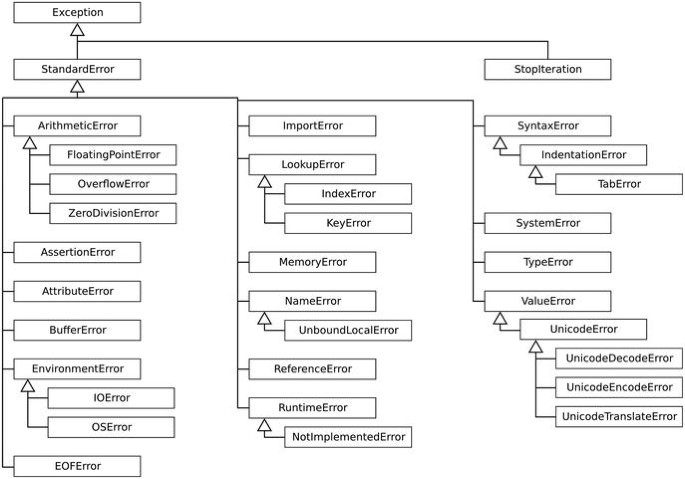
\includegraphics[width=400pt,height=260pt]{slike/419627_1_En_2_Fig4_HTML.jpg}
	\caption{Klasa izuzetaka u programskom jeziku Pajton.}
	\label{fig: exceptions}
\end{figure}

Postoji joše jedan mehanizam koji uslovno aktivira izuzetak, a to je naredba \texttt{assert}. Ona provjerava prov da li je uslov tačan (\emph{True}). U slučaju da nije, izbacuje se poseban tip greške \texttt{AssertionError} aktivirajući navedenu poruku o grešci, gdje se potom izvršavanje narednih dijelova program zaustavlja. Primjer upotrebe naredbe \texttt{assert} je dat sljedećim k\^odom

\begin{minted}{python}
x = 5
assert x > 0, "x is not positive"
\end{minted}

Da zaključimo, rad sa izuzecima je važna praksa u pisanju robusnog koda koji je tolerantan na greške. Izuzeci nam omogućavaju elegantno rješavanje neočekivane situacije koja se javlja pri izvršavanju programa te pruža  korisniku korisne povratne informacije. 

\section{Rad sa datotekama}

Pomoću svojih ugrađenih funkcija, Pajton omogućuje jednostavan rad sa ulaznim i izlaznim datotekama. U nastavku dajemo pregled najčešće korištenih metoda.

\textit{Čitanje iz datoteke}. Koristimo funkciju \textit{open}(), koja ima dva argumenta -- naziv datoteke (ili putanja do datoteke) i način u kojem se otvara datoteka (npr. za čitanje, pisanje, dodavanje, itd.). Pogledajmo sljedeći primjer: 
\begin{minted}{python}
# Otvaranje fajla za citanje
file = open("datoteka.txt", "r")
# Citanje sadrzaja iz fajla 
sadrzaj = file.read()
# Zatvaranje fajla
file.close()
# Ispisivanje sadrzaja fajla 
print(sadrzaj)
\end{minted}

Dakle, prvo otvaramo datoteku  \texttt{datoteka.txt} samo za čitanje. Zatim čitamo sadržaj datoteke koristeći metodu \textit{read}() i čuvamo ga u varijabli \textit{sadrzaj}. Konačno, zatvaramo datoteku pomoću metode \textit{close}() i ispisujemo sadržaj datoteke. 



\textit{Pisanje u fajl}. Za pisanje u datoteku koristimo funkciju \textit{open}(), koja otvara fajl sa određenim nazivom, ali ovaj put sa načinom ``\textit{w}" (eng. write), čime se dopušta pisanje u fajl. Pogledajmo sljedeći primjer.
\begin{minted}{python}
# Otvaranje fajla za pisanje
file = open("datoteka.txt", "w")
# Pisanje teksta u datoteku
file.write("Zdravo!")
#  Zatvaranje fajla 
file.close()
\end{minted}


\textit{Dodavanje u fajl}. Da biste dodali sadržaj u postojeći sadržaj datoteke, otvaramo fajl sa načinom ``\textit{a}" (eng. append), a potom pomoću funkcije \textit{write}() upisujemo novi sadržaj na postojeći. 

Napomenimo da je dobra praksa zatvoriti datoteku nakon što završite rad sa njom, kako bismo izbjegli bilo kakve potencijalne probleme sa oštećenjem datoteke ili gubitkom podataka. Praksa je da se rad u fajlovima odvija pod \textit{try}-\textit{except} blokom. Klase izuzetaka koje se u tim slučajevima mogu koristiti su: \texttt{FileNotFoundError} i \texttt{OSError}. 

% Upis json, csv, ispis itd. 

\subsection{Modul Json}

Modul \texttt{json} se koristi  za kodiranje i dekodiranje podataka sa i u JSON format (eng. \textit{Java Script Object Notation}) formatu. JSON je  široko rasprostranjen format za razmjenu podataka, ljudima jednostavan za čitanje i pisanje, a mašinama za raščlanjivanje i generisanje.

Modul \texttt{json} nudi dvije glavne metode za rad sa JSON podacima:


\begin{itemize}
	\item json.\textit{dump}() -- koristi se za kodiranje pajton objekata u JSON format i njegovo spremanje u objekat  datoteka.
	\item json.\textit{loads}() -- koristi se za dekodiranje JSON niza u pajtonov objekat (obično heš mapa).
\end{itemize}

Pogledajmo i jedan primjer upotrebe \texttt{json} modula. 

\begin{minted}{python}
	import json
	
	# Pajton objekat
	objekat = {'ime': 'Mirko', 'godine': 30, 'grad': 'Banja Luka'}
	# Enkoduj objekat u JSON string
	json_string = json.dumps(objekat)
	# Dekodiraj JSON string nazad u pajtonov objekat (dict)
	dekodiran_objekat = json.loads(json_string)
	
	print(type(json_string))   # <class 'str'>
	print(type(dekodiran_objekat))   # <class 'dict'>
	print(dekodiran_objekat)    # {'ime': 'Mirko', 'godine': 30,
		                        # 'grad': 'Banja Luka'}
\end{minted}


Primijetite da funkcija \textit{dumps}() pretvara pajtonov objekat u string (kodiranje), dok funkcija \textit{loads}() radi obrnutu stvar, od stringa pravi pajtonov objekat (enkodiranje). 

\section{Regularni izrazi}

U ovoj sekciji izlažemo uoptšteno o regularnim izrazima. Potom, će biti riječi o pajtonovom modulu \texttt{re} specijalno namijenjenog za rad sa regularnim izrazima. Na kraju ćemo dati nekoliko primjera upotrebe ovog modula. 

\subsection{Uopšteno o regularnim izrazima}

Regularni izraz ili \textit{regex} (šablon ili patern) je niz znakova koji opisuju skupove nizova znakova, na osnovu određenih žsintaksnih pravila. U prevodu to je šablon koji opisuje neki skup stringova.  Svrha regirarnih izraza je opisivanje uzorka za pretraživanje nizova znakova konciznim opisom bez nabrajanja svih elemenata (stringova) skupa. Npr. kako koncizno opisati sve binarne nizove
pomocu šablona ili kako koncizno opisati skup \{\texttt{gray}, \texttt{grey}\} (engleski i
americki engleski za istu riječ)? Regularne izraze koriste razni uređivači teksta, kao što je filter \textit{grep} u Unix-u, itd. 

Osnovni koncepti regularnih izraza su:
\begin{itemize}
	\item \textit{Alternacija} -- izražava se pomoću znaka $\mid$, te označava sve alternativne mogućnosti koje se mogu uzeti; npr. regluarni izraz $a\mid b\mid c$ označava skup riječi $\{a, b, c\}$.  
	\item \textit{Zagrada} -- označava grupisanje, tj. područje djelovanja. Npr. \texttt{gr}(a$\mid$e)\texttt{y} označava patern kojim u obuhvaćeni riječi \texttt{gray} i \texttt{grey}.
    \item \textit{Specijalni karakteri i skup karaktera}:
    \begin{itemize}
    	\item ``$.$'': sparuje bilo koji karakter samo jednom; 
    	\item $[]$: sparuje bilo koji karakter pod (uglastim) zagradama samo jednom. Npr. ako želimo da označimo skup sva malih slova, odgovarajući patern bi bio [$a-z$], dok bismo velika označili sa [$A-Z$], a jedna i druga sa [$a-zA-Z$]
    	\item $\backslash d$: sparuje bilo koju cifru samo jednom. Drugi način je koristiti patern sa zagradama: [$0-9$];
    	\item $[\^ \  ]$: sparuje bilo koji karakter tačno jednom koji pripada komplementu skupa karaktera pod
    	uglastim zagradama; 
    	\item $\backslash w$: sparuje bilo koji karakter riječi (slova, brojevi ili povlaka); 
    	\item $\backslash n$: sparuje novi red;
    	\item $\backslash s$: sparuje blanko simbol; 
    	\item $\backslash b$: sparuje granicu riječi -- položaj između znaka riječi i znaka koji nije riječ, kao što je razmak, interpunkcija oznaka ili početak/kraj reda;
    	\item $\backslash t$, $\backslash .$, $\ldots$.
    \end{itemize}
	\item  \textit{Kvantifikatori} -- navode se nakon znaka ili grupe, i oni određuju  učestalost
pojavljivanja izraza koji prethodi kvantifikatoru:
\begin{itemize}
	\item ``?'': izraz prije pojavljivanja kvantifikatora se pojavljuje 0 ili 1 puta; % -- colou?r
	\item ``*'': izraz prije pojavljivanja kvantifikatora se pojavljuje 0 ili više puta;
	\item  ``+'': izraz prije pojavljivanja kvantifikatora se pojavljuje  1 ili više puta;
	\item $\{m,n\}$: izraz prije ovog kvantifikatora se pojavljuje od $m$ do $n$ puta (uključujući i granične vrijednosti).
\end{itemize}
\end{itemize}

Reguaran izraz za registarske tablice automobila su date u formatu tri broja, potom povlaka, pa jedno (veliko) slovo, pa potom tri broja, što odgovara regularnom izrazu:
$$ \backslash d \{3\}-[A-Z]-\backslash d\{3\}$$

Regularni izraz za definisanje datum rođenja (sa vodećim nulama za jednocifreni dan i mjesec rođenja; npr. 1 se označava sa 01) izgleda ovako:
$$(\backslash d \{2\})\backslash.(\backslash d \{2\})\backslash.(\backslash d \{4\})\backslash. $$ 

\subsection{Modul Re}
Modul \texttt{re}  je ugrađeni modul koji je namijenjen za rad sa regularnim izrazima. Ovaj modul omogućuje programerima da izrade i primjenjuju regularne izraze, te da se efikasno nalaze paterni u tekstu koji se uklapaju u njih. 

Neke od metoda modula \texttt{re} su date u nastavku.
\begin{itemize}
	\item Metod \textit{search}(pattern, str): pretraživanje niza znakova za određen \textit{pattern} u tekstu \textit{str}.
	\item Metod \textit{match}(pattern, str): pronalaženje  uzoraka na osnovu obrasca \textit{pattern} iz niza znakova \emph{str}; vraćanje po redoslijedu pojavljivanja   uzorka se vrši primjenom funkcije \emph{group}() na objekat vraćen prethodnom funkcijom, (Vrijednost argumenta koji se prosljećuje označava redni broj uzorka koji se izdvaja.)
	
	\item Metod \textit{sub}(pattern, strChange, str): mijenja sva podudaranja obasca \textit{pattern} sa drugim nizom znakova (\textit{strChange}) u stringu \texttt{str}.
	%\item Provjera je li je niz znakova u skladu s određenim regularnim izrazom.
	\item Metod \textit{split}(pattern, str): razdvaja  niza znakova stringa \emph{str} na osnovu  obrasca \emph{pattern}, te vraća niz razdvojenih (pod)stringova.
\end{itemize}
 
 U nastavku navodimo jedan primjer primjene modula \texttt{re} i funkcije \textit{search}().
 
 \begin{minted}{python}
 	import re
 	# definiranje uzorka koji se traži
 	pattern = r'\b\w+'
 	# niz znakova za pretraživanje
 	text = 'Hello, World!'
 	# pretraživanje po obrascu
 	match = re.search(pattern, text)
 	# ispis (prvo) podudaranje
 	print(match.group()) 
\end{minted}

 Drugim riječima, odgovara bilo kojem nizu jednog ili više uzastopnih znakova riječi   kojima prethodi granica riječi (položaj između znaka riječi i znaka koji nije riječ, kao što je razmak, oznaka interpunkcije ili početak/kraj reda.
 
\section{Moduli Sys i Getopt}

\textit{Pokretanje programa preko terminala}. Pokretanje pajton skripte preko terminala se izvršava na sljedeći način:

\begin{minted}{python}
 python myscript.py arg1 arg2
\end{minted}
gdje se komanda \emph{python} (ili \textit{python3},  ako je instalirana pajtonova verzija 3.0 ili viša) postavlja preko  varijable okruženja \texttt{PYTHONPATH}. 

 Modul \texttt{sys} omogućuje pristup nekim parametrima i funkcijama specifičnim za sistem. 

Neke od često korištenih funkcija i atributa \texttt{sys} modula su:

\begin{itemize}
	\item \textit{argv}: Lista argumenata komandne linije proslijeđenih pajtonovoj skripti. Na indeksu 0 se čuva naziv same skripte, dok se na ostalim indeksima čuvaju vrijednosti proslijeđenih parametara. 
     \item \textit{path}: Vraća listu stringova koji specificiraju stazu do pojedinih modula. Inicijalizuje se iz varijable okruženja PYTHONPATH i zadate vrijednosti koja zavisi o instalaciji pajtona.
     \item \textit{exit}([arg]): Izlazak iz pajtonovog inetrpretera sa opcionim izlaznim k\^odom. Ako je dat \textit{arg}, on se koristi kao izlazni k\^od; inače je zadani izlazni kod nula.
     \item \textit{version}: Niz koji sadrži verziju pajtonovog interpretera.
     \item \textit{platform}: Niz koji identikuje platformu operativnog sustava.
\end{itemize}

U nastavku slijedi nekoliko programa koji pokazuju rad sa \texttt{sys} modulom. 

\begin{minted}{python}
import sys
if len(sys.argv) > 1:
    print("Argumenti komandne linije su:")
    for arg in sys.argv[1:]:
        print(arg)
else:
    print("Nema proslijeđenih argumenata komandne liniije.")
\end{minted}

Izvršavanjem prethodnog programa dobijamo izlaz:
\begin{minted}{python}
Argumenti komandne linije su:
arg1
arg2
\end{minted}

Modul \texttt{getopt} predstavlja parser argumenata komandne linije. Omogućuje  pisanje skripti koje mogu uzimati argumente i opcije iz komandne linije pri izvršavanju programa. Modul \textit{getopt} ima dvije bitne funkcije, \textit{getopt}() i \textit{getopt\_long}(), koje se koriste za analiziranje argumenata komandne linije. 

Funkcija \textit{getopt}() analizira kratke opcije (opcije od jednog slova) i vraća torku od dva elementa:

\begin{itemize}
	\item prvi element je lista parova (opcija, vrijednost); 
	\item drugi element je lista argumenata preostalih nakon uklanjanja opcija.
\end{itemize} 
 
Funkcija getopt\textit{\_long}(), sa druge strane, analizira duge opcije (opcije sa više slova) i vraća torku od dva elementa: 
\begin{itemize}
	\item  prvi element je lista parova (opcija, vrijednost);
	\item  drugi element je lista argumenata koja preostaje nakon uklanjanja opcija.
\end{itemize}

Kratke opcije stoje u formatu stringa slova koje odgovaraju opcijama. 
U slučaju kratkih opcija koje zahtijevaju unos vrijednosti, u nastavku stoji ``:''. 
Npr. ako imamo ``hi:o:'' koja odgovara kratkim nazivima opcija, to znači da su uz argumente -$i$ i -$o$ obavezne vrijednosti, dok argument -$h$ može da stoji samostalno. 
  
Duge opcije stoje u obliku liste naziva opcija (zapisane pomoću stringa). 
U slučaju dugih opcija koje zahtijevaju unos vrijednosti, na kraju svake opcije stoji ``=''.  U nastavku slijedi primjer korišćenja modula \texttt{getopt}.

\begin{minted}{python}
import getopt
import sys

def main(argv):
    inputfile = outputfile = ''
    try:
        opts, args = getopt.getopt(argv,"hi:o:",["ifile=","ofile="])
    except getopt.GetoptError:
        print('test.py -i <inputfile> -o <outputfile>')
        sys.exit(2)
    for opt, arg in opts:
        if opt == '-h':
                print('test.py -i <inputfile> -o <outputfile>')
                sys.exit()
        elif opt in ("-i", "--ifile"):
                inputfile = arg
        elif opt in ("-o", "--ofile"):
                outputfile = arg

print('Input file is "', inputfile)
print('Output file is "', outputfile)

if __name__ == "__main__":
    main(sys.argv[1:])
\end{minted}
U prethodnom primjeru, skripta uzima dva argumenta, -$i$ (ili duže - -\emph{ifile}) za ulazni fajl, te -$o$ (ili duže - -\emph{ofile}) 
za izlazni fajl. U slučaju da korisnik ne proslijedi (obavezne) argumente, skripta će ispisati poruku o greški -- aktiviraće se izuzetak \texttt{GetoptError} koji pripada modulu \texttt{getopt}. 

 Da bi pokrenuli skriptu (naziva test.py), na komandnoj liniji unosimo sljedeći kod:
 \begin{minted}{python}
python3 test.py -i ulaz.txt -o izlaz.txt
 \end{minted}
 Nakon pokretanja skripte, prikazaće se sljedeće:
 \begin{minted}{python}
 Input file is " ulaz.txt
 Output file is " izlaz.txt
 \end{minted}

\section{Modul Numpy}

Ovaj modul je specijalizovan za rad sa nizovima i nizovnim strukturama kao što su
matrice, 3D matrice, proizvoljne matrice,  velikih dimenzija. Riječ \texttt{numpy} predstavlja skraćenicu  engleske fraze \emph{numerical python}.  Kreirana je 2005. od strane Travisa Oliphanta, a napisana je u jezicima C/C++. Jedan numpy  objekat predstavlja neprekidan (statičan) dio u memoriji, a za razliku od liste, ovaj objekat je homogene strukture, vidjeti Sliku 	\ref{fig:numpy_array}. Zbog svega toga, pogodan je   za rad  sa velikim tipovima podataka, i brži je za red velicine (oko 50 puta) od tradicionalne liste.

\begin{figure}%https://stackoverflow.com/questions/57262885/how-is-the-memory-allocated-for-numpy-arrays-in-python
	\centering
	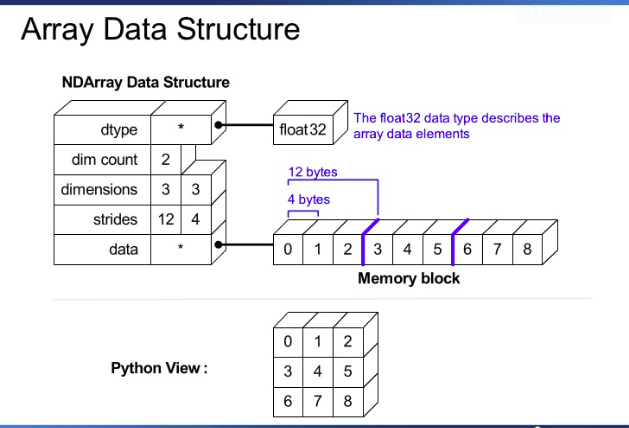
\includegraphics[width=250pt,height=170pt]{slike/numpy_array.png}

	\caption{Struktura podataka numpy niza.}	 \label{fig:numpy_array}
 
\end{figure} 

\textit{Inicijalizacija objekta}. 
\begin{minted}{python}
import numpy as np
ar = np.array([2, 4, 1, 10], dtype="int32") # niz
matrica = np.array([[2, 5 ], [1, 7] ], dytpe="int32") # matrica (2D-niz)
matrica3D = np.array( [[[2, 5 ], [1, 7] ], [[2, 3], [5, 5]]], \ 
dytpe="int32") # 3D matrica
\end{minted}
 
Što se tiče eksplicitno definisanog tipa elemenata objekta numpy (argument \emph{dtype}) mogući su sljedeći tipovi:  $i$: integer (i4, i2, itd.),  $b$: boolean, $u$: unsigned integer, $f$: float,  $M$: datetime, $O$: object, $S$: string. 

\textit{Osnovne metode}.
\begin{itemize}
	\item  Vraćanje elementa na određenoj poziciji (indeksu): 
	\begin{itemize}
		\item 1D niz:  [indeks]
		\item 2D niz:  [indeks1, indeks2]
		\item 3D niz: [indeks1, indeks2, indeks3]
	\end{itemize}
    \item \textit{shape}(): vraćanje dimenzije niza;  
    \item Izrezivanje (\textit{slicing}):  [start:end:step]: slično kao i kod listi; 
    \item Kopiranje niza: funkcija \textit{copy}() koja se primjenjuje na objekat koji se kopira (tačka notacija);
    \item \textit{reshape}(): promjena dimenzije niza, potrebna je kompatibilnost broja
    elemenata početnog niza sa izmijenjenom dimenzijom; 
    \item \textit{np.concatenate}( ($arr1, arr2$), $axis=$.): spajanje dva numpy objekta   
    po $x$ ili $y$ osi (argument axis ili 0 ili 1) 
    \item  \textit{np.array\_split}($arr, n, axis$): dijeljenje niza \textit{arr} na više manjih nizova, gdje je $n$ broj nizova na koje dijelimo niz, dok je  \textit{axis} osa po kojoj želimo da vršimo dijeljenje;
    \item  \textit{where}(uslov): vraća niz indeksa onih elemenata niza koji se uklapaju u \textit{uslov}; npr. uslov može biti: $arr$== 4 ili $arr$ \% 2 == 0;
    \item \textit{np.sort}(\emph{arr}): sortiranje niza \emph{arr};
    \item Filtriranje elemenata u nizu se može izvesti na sljedeći način
    \begin{minted}{python}
arr = np.array([41, 42, 43, 44])
filter_arr = arr > 42
newarr = arr[filter_arr]
    \end{minted}
    \item \textit{numy.zeros}(dim), \textit{numpy.ones}(dim): kreiranje matrice dimenzije dim sa svim nulama, odnosno jedinicama.
\end{itemize}

 \textit{Memorijska organizacija}. Slika~\ref{fig:numpy_array} daje pojednostavljeni prikaz memorijske organizacije numpy objekta u jeziku Pajton.  Ovaj objekat pripada klasi \texttt{ndarray}, koja ima nekoliko bitnih atributa: 
 \begin{itemize}
 	\item \textit{dtype}: definiše tip podataka elemenata koji se smještaju u strukturi.
 	\item \textit{dim\_count}: definiše dimenzionalnost objekta (2D, 3D, isl.).  
 	\item \textit{dimensions}: definiše dimenzije po svakoj od koordinata.  
 	\item \textit{strides}: torka koja definiše broj bajtova koje treba pomaknuti u memoriji da bi se pristupilo sljedećem elementu u nizu duž određene dimenzije. Npr. za 2D niz, \textit{stride} torka je definisana sa (bajt\_za\_pomicanje\_u\_smjeru\_reda, bajt\_za\_pomicanje\_u\_smjeru\_kolone). 
 	\item \textit{data}: pokazivač na sadržaj niza. 
 \end{itemize} 
 

\section{Modul Ctypes}

Modul \textit{ctypes} pruža način za pozivanje funkcija i korištenje tipova podataka u dijeljenim  bibliotekama ili bibliotekama dinamičkog povezivanja (DLL) napisanim u jeziku \textit{C} ili drugim jezicima nižeg nivoa unutar pajtonovog koda. Osnovni  koraci za korištenje \textit{ctypes} modula za uključivanje \textit{C} programa u pajtonov kod su dati u nastavku.

\begin{enumerate}
	\item Prvo  napisati \textit{C} program koji želimo ugraditi u pajtonov   k\^od. Ovaj program može da sadrži jednu ili više funkcija koje želimo pozvati unutar k\^oda pisanog u Pajtonu.
	\item Prevesti (kompajlirati) \textit{C} program u dijeljenu biblioteku.    Na Linuks ili macOS  sistemima u tu svrhu koristimo \textit{gcc} kompajler. Na sistemu Windows možete koristiti Visual Studio ili MinGW za kompajliranje programa u DLL fajl.
	\item Učitati dijeljenu biblioteku u pajtonov k\^od. Ovaj proces vršimo uz  pomoć modula \texttt{ctypes}. Učitavamo .dll fajl pozivanjem funkcije \textit{cdll.LoadLibrary(path)} gdje je \textit{path} proslijeđena staza do dijeljene (dll) biblioteke.
	\item Definišimo tipove argumenata i ono što vraćaju funkcije napisane u \textit{C} programu. Prije nego što   pozovemo \textit{C} funkciju iz pajton programa pomoću modula \texttt{ctypes}, ttrebaju se navesti tipovi argumenata i tipovi koje funkcije vraćaju. To možemo učiniti postavljanjem \textit{argtypes} i \textit{restype} atributa funkcijskog objekta.
	\item Pozivanje \textit{C} funkcije u pajtonovom programu: Na kraju, pozivamo \textit{C} funkciju iz pajtona pomoću funkcijskog objekta koji je kreiran u koraku 4. Vrijednosti argumenata proslijeđujemo kao pajtonove objekte, a modul \texttt{ctypes} će ih automatski pretvoriti u odgovarajuće \textit{C} tipove podataka. 
\end{enumerate}

U nastavku navodimo čitav proces   poziva \textit{C} programa izvršavanjem pajtonovog koda.


\begin{minted}{C}
	// dodaj.c
	int saberi(int a, int b) {
		return a + b;
	}
\end{minted}

Kompajlirajmo \textit{C} k\^od pomoću \textit{gcc} kompajlera:
\begin{minted}{C}
	  gcc -shared -o lib_dodaj.so dodaj.c
\end{minted}
Dalje, učitavamo kreirani dijeljeni fajl u pajtonov program pomoću  \texttt{ctypes} modula:
\begin{minted}{python}
	import ctypes
	lib_dodaj = ctypes.cdll.LoadLibrary('./lib_dodaj.so')
\end{minted}
Potom, eksplicitno definišemo tipove argumenata i tip koji vraća odabrana \textit{C} funkcija:
\begin{minted}{python}
	saberi_func = lib_dodaj.saberi
	saberi_func.argtypes = [ctypes.c_int, ctypes.c_int]
	saberi_func.restype = ctypes.c_int
\end{minted}
Konačno, pozovemo odabranu \textit{C} funkciju uz pomoć k\^oda:
\begin{minted}{python}
	result = saberi_func(2, 3)
	print(result)   # Output: 5
\end{minted}

 
\section{Pisanje prilagodjenih modula}

Pretpostavimo da želimo kreirati modul koji služi za različite matematičke operacije, kao što su sabiranje, oduzimanje, množenje i dijeljenje. Kako smo pomenuli, modul je skup objekata koji se  čuva u datoteku ekstenzije .\textit{py}. Pretpostavimo da želimo kreirati modul \textit{mathOps}. Dakle, kreirajmo  datoteku pod nazivom ``\textit{mathOps}.py" i tamo definišemo funkcije ovog prilagodjenog modula. Evo primjera kako bi ta datoteka mogla izgledati:

\begin{minted}{python}
def add(x, y):
    return x + y

def subtract(x, y):
    return x - y

def multiply(x, y):
    return x * y

def divide(x, y):
    if y == 0:
        raise ValueError("Ne možemo dijeliti sa 0")
    return x / y
\end{minted}
Ovaj  primjer definiše četiri različite funkcije, od kojih svaka izvodi različite matematičke operacije. Funkcija \textit{add} uzima vrijednost dva argumenta, $x$ i $y$, i vraća njihov zbir. Funkcija \textit{subtract}   vraća razliku dva broja koji se prenose kao argumenti funkcije. Funkcija \textit{multiply} vraća proizvod dva broja. Konačno, funkcija \textit{divide} uzima dva argumenta, i vraća rezultat njihovog dijeljenja, ali takođe  javlja  grešku ako je nazivnik (vrijednost argumenta $y$) nula.

Korištenje ovog prilagodjenog modula u drugoj pajtonovoj datoteci se vrši importovanjem modula \textit{mathOps} na sljedeći način:

\begin{minted}{python}
import mathOps

result = mathOps.add(3, 4)
print(result)   # Output: 7

result = mathOps.divide(10, 2)
print(result)   # Output: 5.0

result = mathOps.divide(10, 0)
# Output: ValueError: Ne možemo dijeliti sa 0
\end{minted}

U ovom primjeru uvozimo modul ``\textit{mathOps}" i koristimo njegove funkcije za izvođenje matematičkih operacija. Pozivamo funkciju  \textit{add}  koja vraća zbir brojeva 3 i 4, a to je 7. Zatim pozivamo funkciju  \textit{divide}  za dijeljenje 10 sa 2, koja vraća 5,0. Na kraju, ponovno pozivamo funkciju  \textit{divide}  da bismo podijelili 10 sa 0, što uzrokuje \texttt{ValueError} jer dijeljenje sa nulom nije dopušteno.


\section{Postavljanje korisnički kreirani modul  na PyPI repozitorij}

PyPI (\textit{Python Package Index}) je centralni repozitorij paketa   koji su pisani u programskom jeziku Pajton. PyPI omogućuje programerima lako distribuiranje korisnički napisanih modula,  omogućavajući da dati paket bude korišten široj zajednici korisnika.
 
Nekoliko   koraka   treba izvršiti ukoliko želimo postaviti   korisnički kreirani modul na PyPI repozitorij. Na zvaničnoj PyPI veb stranici, na linku  \url{https://pypi.org/account/register/},  potrebno je kreirati račun. Nakon što se prijavimo, potrebno je  generisati token za prijavu na PyPI. Token je sigurnosni ključ koji omogućuje da se prijavimo i objavimo  paket (modul). 
 
 
 Na lokalnom računaru instalirajmo module  \texttt{setuptools} i \texttt{wheel}, u slučaju da nisu instalirani. To se možete učiniti pomoću \textit{pip} naredbe:
 \begin{minted}{python}
      pip install setuptools wheel
 \end{minted}

Modul \texttt{setuptools} omogućuje da upravljamo i distribuiramo naš modul, a modul \texttt{wheel}   omogućuje generisanje datoteka sa ekstenzijom .\textit{whl} koje se mogu lako instalirati.

Potom,  u korijenom direktorijumu našeg modula  kreiramo fajl \textit{setup.py}. Fajl \textit{setup.py}  definiše informacije o našem modulu kao što su naziv, verzija, autor, opis i druge metapodatke koji će biti prikazani na PyPI stranici   modula. Primjer takvog fajla je dat u nastavku.

\begin{minted}{python}
   from setuptools import setup
   
   setup(
   name='modul1',
   version='0.0.1',
   author='Mirko Mirkovic',
   description='modul1',
   packages=['modul1'],
   install_requires=[
   'numpy',
   'pandas'
   ]
   )
\end{minted}
Ovaj \textit{ setup.py}   definiše paket ex\_package sa verzijom 0.0.1, datim autorom  i opisom, a zavisi od modula \textit{numpy} i \textit{pandas}.

Naredni korak je kreiranje distribucijske datoteke (source distribution i wheel distribution) pomoću \texttt{setuptools}, izvršavajući naredbu:
\begin{minted}{python}
        python setup.py sdist bdist_wheel
\end{minted}
 
Dalje instaliramo \texttt{twine} paket, koji će pomoći da postavimo naš distribucijski modul na PyPI repozitorijum. Instaliramo ga pomoću   naredbe:
\begin{minted}{python}
	pip install twine
\end{minted}
Potom postavimo korisnički   modul na PyPI pomoću twine naredbe:
\begin{minted}{python}
	twine upload dist/*
\end{minted}
Izvršavanje prethodne naredba će tražiti da se unese PyPI korisničko ime i lozinka, a zatim će prenijeti      paket na PyPI (direktorijum dist).

Nakon  objave  modula na PyPI, možemo ga instalirati pomoću   naredbe:
\begin{minted}{python}
	pip install modul1
\end{minted}


\section*{Zadaci}
%regularni izrazi:
\begin{enumerate}
    %%https://adriann.github.io/programming_problems.html
    
    \item Implementirajte igru pogađanja u kojoj korisnik treba da pogodi skriveni broj. Nakon pogađanja, program izvještava korisnika da li je njegov broj velik ili mali (ili je pogođen). Na kraju ispisati broj  pokušaja iz kojeg je korisnik pogodio skriveni broj. Računa se jedan pokušaj ukoliko se unese isti broj više puta uzastopno.
    
    
	\item Napisati program koji računa sljedeću sumu  
	
	$$ 4 \cdot \sum_{k=1}^{10^6}(-1)^{k-1} \frac{1}{2k-1}= 4 \cdot (1-1/3 + 1/5-1/7+1/9-1/11 \ldots).$$
	
	\item Napisati funkciju koja kombinira dvije liste naizmjenično uzimajući naizmjenično elemente jedne pa druge liste, Npr. za $[a,b,c], [5, 6, 7]$ generišemo listu $[a,5,b,6,c,7]$.
	
	\item Napisati funkciju koja rotira listu za $k$ elemenata. Npr. lista  $[1,2,3,4,5,6]$ rotirano za $k=2$ je data sa $[3,4,5,6,1,2]$. Riješiti zadatak bez kreiranja kopije liste. 
	
	\item Napisati funkciju koja uzima broj i vraća listu njegovih brojeva. Npr. za broj $2342$ treba vratiti listu $[2,3,4,2]$.
	
	\item Napisati funkciju koja uzima listu brojeva,   bazu $b_1$ u kojoj se brojevi liste interpretiraju, te ciljnu bazu $b_2$.  Kao rezultat vratiti listu brojeva konvertujući svaki od brojeva početne liste u bazu $b_2$. Npr. za listu $[21,10,01]$ u bazi $b_1 = 3$ pretvaramo u listu brojeva po bazi $b_2=10$, dobijajući $[7,3, 1]$.
	
	\item Napišite funkciju koja množi dvije matrice.
	 
	\item Napisati regularni izraz koji prepoznaje registarske tablice. Testirati primjenu uz pomoć modula \texttt{re}.
	
	\item Napisati regularni izraz koji prepoznaje imejlove. Testirati primjenu uz pomoć modula \texttt{re}.
	
	\item Napisati regularni izraz koji prepoznaje realne brojeve. Testirati primjenu uz pomoć modula \texttt{re}.
	
	
	\item Kreirati datoteku \textit{apsolventi}.txt i popuniti je podacima gdje je u svakom redu data
	informacija o studentu apsolventu u formi: 
	 $$<Ime\_prezime>, <datum\_upisa\_na\_fakultet>, <godine\_starosti>$$ 
	
	Datum se zadaje u formi $<broj>.<broj>.<broj>$. Napisati skriptu koja se pokreće sa terminala čiji su argumenti komandne linije:
	\begin{itemize}
		\item  	\textit{i}: koja zadaje ulazni datoteku (sve zajedno sa putanjom) koja treba da bude učitana u
	program;
	     \item \textit{o}: koja zadaje izlaznu datoteku (sve zajedno sa putanjom) u kojoj se čuvaju rezultati	izvršavanja programa;
	     \item  \textit{z}: koji zadaje zadatak koji treba da bude izvršen i obuhvata sljedeći opseg vrijednosti: 
	     \begin{itemize}
	     	\item  1: U izlaznoj datoteci treba da se ispišu svi apsolventi stariji od 25 godina.
             \item 2: U izlaznoj datoteci treba da se ispišu svi apsolventi koji su upisali fakultet u periodu od 01.01.2014. do 01.01.2015. godine.
	         \item 3: U izlaznoj datoteci treba da se ispiše sortiran niz (koristeći merge sort) studenata po godini života.
	         \item 4: U izlaznoj datoteci treba da se ispiše za svakog studenta koliko godina studira.
	        \item za ostale inpute javiti poruku o neispravnoj opciji (unosu).
	         \end{itemize}
       \end{itemize}
	\textit{Napomena}. Studenta učitati uz pomoć regularnih izraza. Dakle, prazni karakter je
	invarijantna vrijednost što se postiže konstrukcijom odgovarajućeg regularnog izraza pri čitanju redova u datoteci.
	
   \item Kreirati datoteku pretplatnik.txt i popuniti je podacima gdje je u svakom redu
   data informacija o studentu u formi
   
   $$<Ime\_prezime>, <datum\_ugovora>, <cijena\_usluge>$$
   
   Datum se zadaje u formi $<broj>.<broj>.<broj>$, a cijena je decimalni broj. Napisati 
   skriptu koja se pokreće sa terminala sa sljedećim argumentima komandne linije:
   \begin{itemize}
   	\item \textit{i}: koja zadaje ulazni datoteku (sve zajedno sa putanjom) koja treba da bude učitana
   u program;
   \item \textit{o}: koja zadaje izlaznu datoteku (sve zajedno sa putanjom) koja treba da sačuva
   rezultate izvršavanja programa;
    \item \textit{z}: koji zadaje zadatak koji treba da bude izvršen i obuhvata sljedeće vrijednosti:
    \begin{itemize}
    	\item  1: U izlaznoj datoteci treba da se ispišu svi korisnici koji koriste usluge čija je  cijena veća od 15,4 KM. Eliminisati duplikate. 
        \item 2: U izlaznoj datoteci treba da se ispišu svi pretplatnici koji su potpisali ugovor u periodu od 01.01.2022. do 15.01.2023. godine.
        \item  3: U izlaznoj datoteci treba da se ispiše zbir svih cijena za usluge koje koristi svaki od pretplatnika
        \item 4: U izlaznoj datoteci treba da se ispišu sortirane cijene od najmanje do  najveće
        \item za ostale inpute javiti poruku o neispravnoj opciji  (unosu).
         \end{itemize}
   \end{itemize}
   \textit{Napomena}. Pretplatnika učitati uz pomoć regularnih izraza. Npr., smatra se da je unos Marko
   Markovic, $20.2.2022, 8,4$ isti kao Marko Markovic, $20.\ \ 2.2022, 8,\ \ 4$, itd. Dakle, prazni
   karakter je invarijantna vrijednost što se postiže konstrukcijom odgovarajućeg regularnog izraza
   pri čitanju redova u datoteci.
\end{enumerate}
 
\chapter{Algoritamske paradigme}

\textit{Programske paradigme} predstavljaju različite pristupe ili stilove  programiranja koji definišu način na koji programeri dizajniraju, strukturiraju i organizuju  svoj k\^od za rješavanje problema. Postoji nekoliko programskih paradigmi, a svaka od njih zahtjeva  drugačiji način razmišljanja o problemima i rješenjima programiranja.

Neke od najčešćih programskih paradigmi su date u nastavku. 

\begin{itemize}
	\item \textit{Imperativno programiranje}: Ova paradigma uključuje %upotrebu naredbi koji mijenjaju stanje programa, a sastoji se od
	 eksplicitni slijed naredbi koje računar izvršava određenim redoslijedom.
	\item \textit{Funkcijsko programiranje}: Ova paradigma se fokusira na korištenje funkcija za rješavanje problema.  %, sa naglaskom na nepromjenjivosti i izbjegavanju nuspojava.
	\item \textit{Logičko programiranje}: Ova paradigma uključuje programiranje zasnovano na logici i zaključivanju. Posebno je koristan za probleme koji uključuju pravila i ograničenja.
	\item \textit{Objektno orijentirano programiranje}: Ova paradigma uključuje kreiranje objekata koji sadrže  podatke i metode/funkcije koje rade na tim podacima (mijenjajući stanje objekta).
\end{itemize}


Različiti programski jezici često podržavaju jednu ili više paradigmi, a neki jezici dozvoljavaju programerima da po potrebi kombinuju  više različitih  paradigmi. Izbor paradigme programiranja često zavisi od domena problema, složenosti problema i ličnih preferencija i iskustva programera.

Kada je riječ o \textit{algoritamskim paradigmama}, one predstavljaju  pristupe ili metode za dizajniranje algoritama koji rješavaju   računske probleme. Postoji nekoliko algoritamskih paradigmi; svaka  ima svoje prednosti i slabosti. 

Neke od najčešćih algoritamskih paradigmi su date u nastavku pomoću kratkog opisa. 

\begin{itemize}
	\item \textit{Rekurzivni algoritmi} --  uključuje rješavanje problema dijeljenjem na manje (pod)probleme, koji se potom rekurzivno rješavaju. Prekid rekurzije se dešava dolaskom do baznih slučajeva koji rješavaju trivijalne (ili skoro trivijalne) podprobleme. 
	\item \textit{Algoritmi grube sile} (eng.\textit{ brute force}) -- uključuje isprobavanje svakog mogućeg rješenja problema dok se ne pronađe ispravno. Obično se upotrebljava samo za male probleme zbog svoje (ne)efikasnosti.
    \item \textit{ Podijeli i vladaj} (eng. \textit{divide-and-conquer}) --  uključuje podjelu problema na manje podprobleme, rješavanje svakog podproblema nezavisno, a zatim se rezultati  kombinuju da bi se riješio originalni problem. Dakle,  koristi se za efikasno rješavanje problema koji se mogu podijeliti na manje, nezavisne dijelove.
    \item \textit{Pohlepni algoritmi} (eng. \textit{greedy}) --  uključuje donošenje lokalno optimalnog izbora u svakom koraku algoritma u nadi da će to dovesti do globalno optimalnog rješenja. Ova paradigma je često korištena za rješavanje problema optimizacije kao prva opcija zbog soje jednostavnosti ali i toga da ne traži intezivne memorijske niti vremenske resurse. 
    \item \textit{Algoritmi dinamičkog programiranja} (eng. \textit{dynamic programming}) --  uključuje razbijanje problema na manje podprobleme i rješavanje svakog podproblema samo jednom. Kada se podproblem riješi, rezultati podproblema se pohranjuju u odgovarajuću (memorijsku) strukturu.    Često se koristi za probleme sa podproblemima koji se preklapaju.
    \item \textit{Algoritmi vraćanja unazad} (eng. \textit{backtracking}) --  uključuje istraživanje svih mogućih rješenja problema postepenom izgradnjom   i napuštanjem parcijalnog rješenja ako se utvrdi da je netačno (nedopustivo). Često se koristi za probleme koji se mogu predstaviti putem grafa (stanja).
    \item \textit{Randomizirani algoritmi} (eng. \textit{randomized}) --  uključuje uvođenje slučajnosti u algoritam radi poboljšanja performansi ili smanjenja složenosti. Često se koristi za probleme optimizacije ili probleme koji imaju mnogo mogućih rješenja.
\end{itemize}

Različite algoritamske paradigme mogu se   prilagoditi ili međusobno kombinovati za efikasnije rješavanje složenih problema. 

\section{Rekurzivni algoritmi}
    %https://www.geeksforgeeks.org/introduction-to-recursion-data-structure-and-algorithm-tutorials/
    
 Riječ rekurzija potiče od latinske riječi \textit{recurrere}, što doslovno znači vraćanje. U programiranju, funkcija koja u tijelu poziva samu sebe se naziva rekurzivna. Pozivanje iste funkcije unutar same funkcije podrazumijeva sistematično smanjivanje veličine ulaza funkcije koja se poziva,  shodno problemu koji se rješava. Smanjivanje dimenzije ulaza odgovara  rješavanju odgovarajućih podproblema početnog problema rekurzivnim putem. %Potom se kombiniraju rješenja podproblema,   da bi se riješio izvorni problem. 
   Da bi se rekurzija izvršavala u konačnom broju koraka, neophodno je definisati prekidne, tzv. \textit{bazne}, slučajeve rekurzije. Bazni slučajevi su bitni iz razloga što su oni okidač prekida rada rekurzije. 
 
 Prepoznavanje pogodne rekurzije igra bitnu ulogu u rješavanju problema rekurzivnim načinom. Demonstrirajmo sada rekurziju i rekurzivni način rješavajnja problema na jednostavnom problemu računanja $n$-tog parnog prirodnog broja. Neka $f(n)$ predstavlja $n$-ti po redoslijedu parni broj u skupu $\mathbb{N}$. Prvi broj u ovom skupu je 0, pa definišimo $f(0)= 0$. Svaki sljedeći je za dva veći od prethodnog, %(relacija ``biti sljedbenik''), 
 što je definisano rekurzijom: 
 $$f(n) = f(n-1) + 2, n \geq 1, f(0) = 0.$$
  
  Dakle, da bismo izračunali treći parni broj po redu u skupu $\mathbb{N}$, imamo sljedeći niz jednakosti:  
  $$f(3)= f(2) + 2 = f(1) + 2 + 2 = f(0) + 2 + 2 + 2 = 0 + 6 = 6.$$
 
 Dakle, poziv $f(3)$ zahtjeva poziv funkcije $f$ sa vrijednosti 2, koja potom zahtjeva poziv fukcije sa vrijednosti (argumenta) 1, i tako sve do trivijalnog koraka, računanja $f(0)$.  Potom se, vraćanjem unazad, računa vrijednost $f(1)$, pa se pomoću nje računa vrijednost za $f(2)$, dok ne dobijemo rješenje za $f(3)$. Napomenimo da se u programskom jeziku Pajton, za svaki poziv funkcije $f$ formira (lokalni) stek, koji nakon izlaza iz funkcije (vraćanjem rezultata) biva obrisan.  
 
Napomenimo da se rekurzivne funkcije (tzv. linearne, homogene) kao u prethodnom primjeru mogu izraziti preko eksplicitne funkcije u odnosu na veličinu ulaza problema, pa rekurzivni pozivi za njihovo  računanje i nisu potrebni. Jasno se vidi da je gore $f(n)=2n$. 
 
Rekurzija u jeziku Pajton  prethodnog    problema je data u nastavku.

\begin{minted}{python}
	def even(n):
		if n==0:
		   return 0
		return 2 + even(n-1) 
		
	n = input("Unesite broj:")
	print(even(n)) 

\end{minted}

\textit{Kompleksnost rekurzije}. Jasno se vidi da se program izvršava u linearnom $O(n)$ vremenu. \\ \vspace{0.2cm}

Napišimo sada rekurziju za računanje faktorijela broja $n$. Označimo $f(n) = n!$. Iz definicije faktorijela, imamo: 
$$f(n) = n! = n \cdot (n-1) \cdots 2 \cdot 1  = n \cdot (n-1)! = n \cdot f(n-1).$$

Bazni korak rekurzije je $f(1)= 1$. Prema tome, rekurzivna implementacija faktorijel funkcije izgleda ovako:
\begin{minted}{python}
	def fact(n):
		if n == 1:
		   return 1
		return n * fact(n-1)
\end{minted}

Na Slici~\ref{fig:rec_tree}, dato je drvo rekurzije prethodnog programa za konkretan slučaj, $n=5$.

\begin{figure}[H]
	\centering
	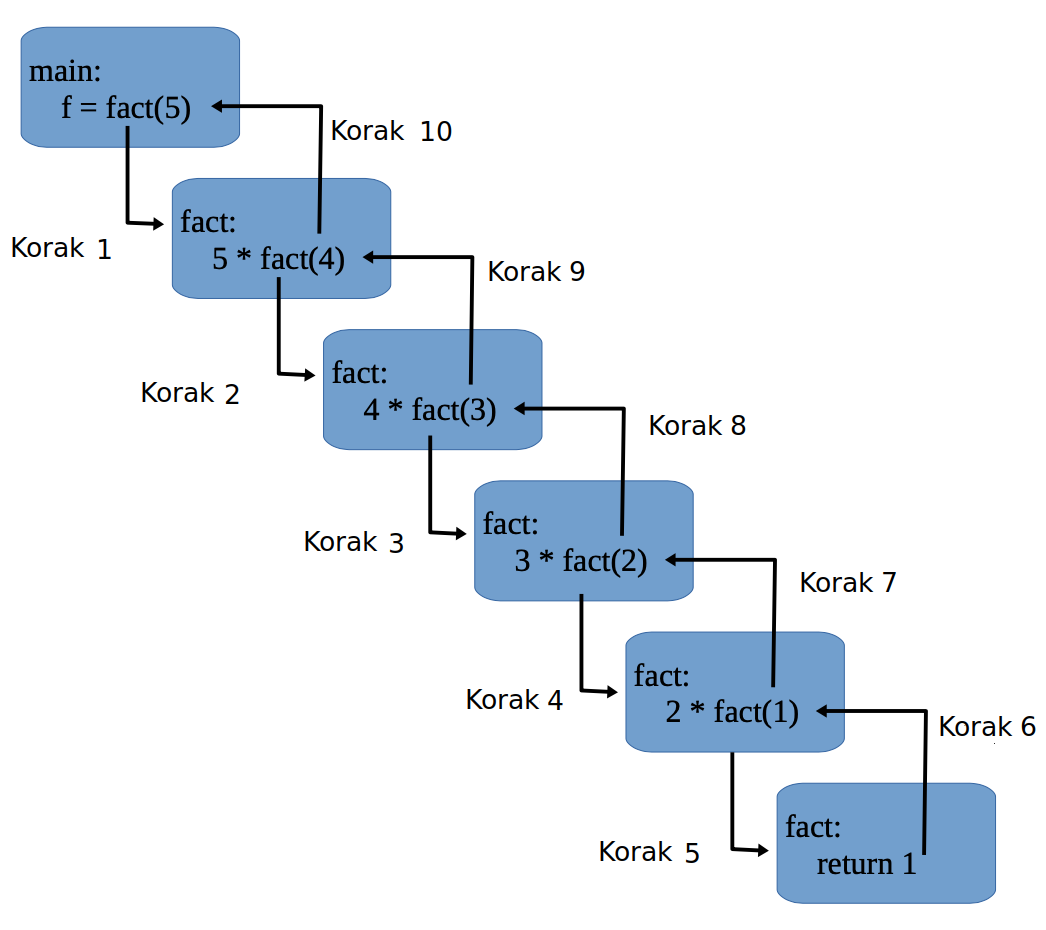
\includegraphics[width=220pt,height=160pt]{slike/factorial_recursion_tree.png} 
	\label{fig:rec_tree}
	\caption{Drvo rekurzije.}
\end{figure}

 


\textit{Kompleksnost rekurzije}. Jasno je da je kompleksnost ove rekurzije linearna, tj. $O(n)$. \\ \vspace{0.2cm}


Ako bazni slučaj nije dostignut ili nije definisan, može doći do problema  prekoračenja steka (eng. \textit{stack overflow}). Posmatrajmo sljedeći program.

\begin{minted}{python}
	def fact(n):
	# pogrešan bazni slučaj 
	if (n == 100): 
	    return 1	
	else:
	    return n*fact(n-1);
\end{minted}

Ovaj program će izazvati prekoračenje steka u slučaju kada je ulaz $n<100$;  tada bazni slučan nikada neće biti ispunjen i rekurzija će se pozivati dok god se ne iscrpi memorija steka rezervisana za program.

\section{Vrste rekurzija}

Funkciju  nazivamo \textit{direktnom} rekurzivnom ako ona poziva istu funkciju. Funkcija \texttt{fun} se naziva \textit{indirektnom} rekurzivna ako poziva drugu funkciju koja potom poziva direktno ili indirektno funkciju \texttt{fun}. Razlika između direktne i indirektne rekurzije ilustrovana je data u narednom programu.

\begin{minted}{python}
	# Direktna rekurzija
	def direktnaRecFunc():
	    # Kod ....
	
	    direktnaRecFunc()
	
	    # Kod...
	
	# Indirektna rekurzija
	def indirektnaRecFun1():
	    # Kod ...
	
	    indirektnaRecFun2()
	
	    # Kod...
	
	def indirektnaRecFun2():
	
	    # Kod...
	
	     indirektnaRecFun1()
	
	     # Kod...
\end{minted}



Rekurzivna funkcija se naziva \textit{repnom} rekurzijom ako je rekurzivni poziv posljednji dio koda koju funkcija izvršava. Inače, rekurzivna funkcija se naziva \textit{nerepnom}.
 
\subsection{Prednosti i nedostaci rekurzivnog nad iterativnim pristupom}

Svaka rekurzija se može napisati na ekvivalentan, iterativni pristup. 
Iako rekurzija i iteracija u ugnježdenim petljama na prvi pogled djeluju dosta slično postoje značajne, suštinske razlike:
\begin{itemize}
	\item Rekurzija se prekida kada se dostigne bazni slučaj; iteracija se prekida kada uslov postane netačan.
	\item Rekurzija se veže za funkcije, dok se iteracija veže za petlje.
	\item Svaki rekurzivni poziv zahtijeva dodatni prostor koji se alocira u memoriji steka; iteracija ne zahtjeva dodatni memorijski prostor.
	\item Rekurzija najčešće ima kraći k\^od; iteracije u petlji su često obimnijeg k\^oda. 
	
\end{itemize}


%Iz ranijih kurseva osnova programiranja je poznato da rekurzivni i iterativni programi imaju istu moć rješavanja problema, tj. svaki rekurzivni program može se napisati u  iterativnom obliku i obrnuto. 

Rekurzivni program ima veće zahtjeve za prostorom od (ekvivalentnog) iterativnog programa, jer će sve funkcije ostati na steku dok se ne dostigne bazni slučaj. Takođe,  zahtjevi za vremenom su veći zbog poziva funkcija i   troškova vraćanja rezultata. Dodatno, zbog manje dužine k\^oda, kodovi znaju biti teški za razumevanje i stoga je potrebno uložiti  dodatnu pažnju prilikom pisanja k\^oda zbog mogućih previda. %Računar može ostati bez memorije ako rekurzivni pozivi nisu ispravno provjereni.

Prednost korištenja rekurzija je u čistom i jednostavnijem načinu pisanja k\^oda. Neki problemi su inherentno rekurzivni, npr. obilazak stabala, problem hanojskih kula, itd. Za takve probleme, poželjno je, a i intuitivnije,  pisati rekurzivni k\^od. Kako smo već naveli, takve kodove možemo pisati i iterativno uz pomoć strukture podataka steka.

\subsection{Primjene rekurzivnog pristupa}

Rekurzija je moćna tehnika sa raznim primjenama u informatici i programiranju. Neke od uobičajenih primjena rekurzije uključuju:

\begin{itemize}
	\item  \textit{Prelazak stabla i grafa}. Rekurzija se često primjenjuje za prelazak i pretraživanje značajnih struktura podataka kao što su stabla i grafovi. Rekurzivni algoritmi se mogu koristiti za istraživanje svih čvorova ili vrhova stabla ili grafa na sistematičan način.
	\item \textit{Algoritmi za sortiranje}. Rekurzivni algoritmi se koriste u algoritmima za sortiranje kao što su \textit{quick sort} (brzo sortiranje) i  \textit{merge sort} (sortiranje spajanjem). Ovi algoritmi koriste rekurziju da podijele podatke u manje podliste, sortiraju ih, a zatim ponovo spajaju.
	%\item \textit{Algoritmi zavadi pa  vladaj}: Mnogi algoritmi koji koriste pristup zavadi pa vladaj, kao što je algoritam binarnog pretraživanja, koriste rekurziju da razbiju problem na manje podprobleme.
	\item \textit{Generisanje fraktala}.  Fraktalni oblici i obrasci mogu se generirati korištenjem rekurzivnih algoritama. Npr. Mandelbrotov skup se generiše uzastopnom primjenom rekurzivne formule na kompleksne brojeve.
	
	\begin{figure}
		\centering
		
\includegraphics[width=100pt,height=80pt]{slike/mandelbrot.png}
		\caption{ Mandelbrotov skup}
	\end{figure}


	\item \textit{Algoritmi vraćanja unazad}. Algoritmi vraćanja unazad se koriste za rješavanje problema koji uključuju donošenje niza odluka, gdje svaka odluka zavisi od prethodnih. Ovi algoritmi se mogu implementirati korištenjem rekurzije za istraživanje svih mogućih staza i vraćanje unatrag kada se rješenje ne pronađe.
	\item \textit{Memoizacija}.  Ovo je tehnika koja uključuje pohranjivanje rezultata skupih poziva funkcija i vraćanje keširanih rezultata kada se naiđe na pozive funkcija istih ulaza. Memoizacija se može implementirati korištenjem rekurzivnih funkcija koje izračunavaju i keširaju rješenja podproblema.
\end{itemize}

U natavku ove sekcije primijenimo rekurzivni pristup na nekoliko konkretnih problema. 

%Pogledajmo naredni zadatak (o rastu populacije zečeva kroz vrijeme). 
\begin{example}
  
	Pretpostavimo da se zečevi reprodukuju na sljedeći način: par zečeva se na kraju prvog mjeseca života ne razmnožava. Međutim, na kraju drugog i svakog sljedećeg mjeseca oni reprodukuju novi par zečeva. Postavlja se pitanje koliko će novorođenih parova zečeva biti poslije godinu dana (tj. na kraju 12-og mjeseca)?
\end{example}

\begin{solution}
	 
	
	Brojevi parova zečeva čine niz: $0, 1,1, 2,3,5,8,13, 21, \ldots$ 
	
	Lako zaključavamo da je svaki sljedeći broj u nizu jednak zbiru prethodna dva broja, tj. ako je $f(n)$ broj  novorođenih zečeva na kraju $n$-tog mjeseca, onda je 
	$$f(n) = f(n-1) + f(n-2), n \geq 2$$
	gdje je bazni slučaj dat sa $f(0)= 0, f(1) = 1$.
\end{solution}

Ova rekurzija je implementirana sljedećim (Pajton) kodom.

\begin{minted}{python}
	def fib(n):
		if n == 0:
			return 0
		if n == 1:
			return 1
		return fib(n-1) + fib(n-2)
\end{minted}

Dakle, u svakom koraku, ako se ne dođe do trivijalnog koraka, rekurzivni poziv će pozvati dvije nove rekurzije (sa manjim veličinama ulaza). Potom će, vraćanjem rezultata na manjim ulazima, rezultat biti izračunat i za veće ulaze. Rješenje prethodnog zadatka se dobija račinajuću rekurziju za ulaz $n=12$. 

%https://www.quora.com/What-is-the-time-complexity-of-the-simplest-recursive-algorithm-that-finds-the-nth-Fibonacci-number
\textit{Kompleksnost algoritma}. Primijetimo da se u svakom koraku broj poziva duplira u odnosu na prethodni. Brzina opadanja veličine ulaza opada konstantno u odnosu na $n$, pa zaključujemo da je kompleksnost izvršavanja rekurzije eksponencijalna, tj. jednaka $O(2^n)$.

%fib_rec.jpeg
\begin{figure}[H]
	\centering
	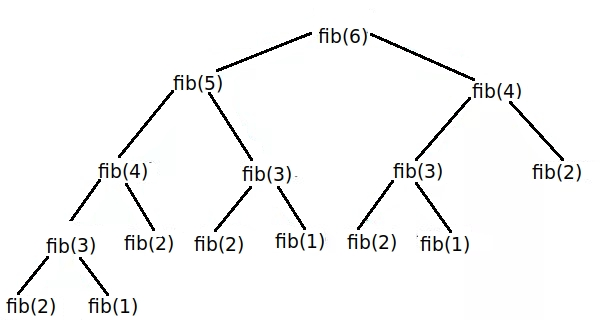
\includegraphics[width=250pt,height=140pt]{slike/fib_rec.jpeg} 
	\label{fig:rec_fib}
	\caption{Drvo rekurzije za \texttt{fib} rekurzivni metod.}
\end{figure}



 %https://www.geeksforgeeks.org/c-program-for-tower-of-hanoi/
 \begin{example}
 	\textbf{\emph{Problem Hanojskih kula}}. Neka su data tri štapa i $n$ diskova. Zadatak ovog problema je u što manje poteza
 	premjestiti diskove sa jednog štapa na drugi štap. Sljedeća pravila vrijede pri prebacivanju diskova. 
 	\begin{itemize}
 		\item Inicijalno, diskovi stoje poredani na jednom štapu ($A$) jedan na drugi gdje  manji diskovi stoje na većim diskovima (pretpostavka je da su diskovi različitih dimenzija). 
 		\item Potez se sastoji od premiještanja jednog diska sa vrha jednog štapa na vrh drugog štapa.   
 		\item Veći disk ne može nikada da bude stavljen na manji disk u bilo kojoj iteraciji premiještanja.
 	\end{itemize}
  \end{example}    

\begin{solution}
 
 
 	Situacija sa dva diska i tri štapa je jasna. Pretpostavimo da se dva diska inicijalno nalaze na štapu $A$ i da ih želimo premijestiti na štap $C$, poštujući uslove zadatka. Označimo ta dva diska crvenom (veći disk) i plavom (manji disk). U prvomu korak prebacujemo plavi disk na štap $B$. Potom crveni disk prebacujemo na štap $C$. Konačno, plavi disk sa štapa $B$ prebacujemo na štap $C$, čime je zadatak završen za slučaj sa dva diska ($n=2$).
 	
 	Posmatrajmo situaciju sa kulama kao na Slici~\ref{fig:tower} sa tri diska ($n=3$) i tri štapa ($A, B$ i $C$). 
 	
 	\begin{figure}[H]
 		\centering
 		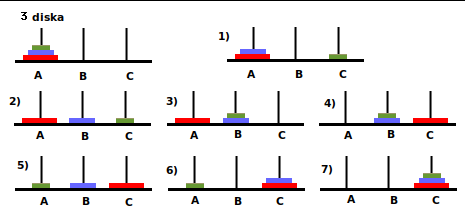
\includegraphics[width=270pt,height=150pt]{slike/tower.png}


 	 \caption{Problem hanojskih kula, $n=3$ diska.}     \label{fig:tower}
 	 	\end{figure}
%\protect\footnotemark\footnotetext{Slika sa linka \url{https://www.geeksforgeeks.org/c-program-for-tower-of-hanoi/}}


 Prvo se najmanji (zeleni) disk prebacuje na štap $C$. Drugi korak je prebacivanje plavog (disk srednje veličine) na štap $B$. Potom, u koraku tri, zeleni disk sa štapa $C$ premiještamo na štap $B$. Korak četiri je rezervisan za prebacivanje najvećeg diska (sa štapa $A$)  na štap $C$. Dalje, potom zeleni disk sa $B$ premiještamo na štap $A$, a plavi na štap $C$. Konačno, u koraku sedam, zeleni disk sa štapa $A$ prebacujemo na štap $C$.  
 
Označimo sa $T(n)$ broj koraka koji je potreban da prebacimo $n$ diskova sa štapa $A$ na štap $C$ koriteći pomoćni štap $B$. Bazni slučaj je $T(1) = 1$. Izvedimo rekurzivni korak za ovaj problem. Kako smo pomenuli, ideja rekurzije je svesti početni problem na rješavanje problema manjih dimenzija (podprobleme) koje ponovo   rekurzivno rješavamo. U ovom slučaju, ``hvatamo'' se za činjenicu da ukoliko je najveći disk sam na jednom štapu, ostalih $n-1$ diskova sa drugog štapa možemo nesmetano prebacivati koristeći sva tri štapa (na veliki disk može da se stavi bilo koji od $n-1$ diskova). Rekurzivno prebacimo $n-1$ diskova sa vrha štapa $A$ na štap $B$, koristeći štap $C$. Nakon toga, situacija je  sljedeća: ($i$) najveći disk se nalazu na štapu $A$; ($ii$) ostalih $n-1$ diskova su složeni na štapu $B$; ($iii$) štap $C$ je prazan. Sljedeći korak je prebacivanje najvećeg diska sa štapa $A$ na štap $C$. Nakon toga, ponovo rekurzivno prebacujemo $n-1$ diskova sa štapa $B$ na štap $C$, koristeći štap $A$. Prema tome, vrijedi rekurzija:
$$ T(n) = 2 \cdot T(n-1) + 1, T(1) = 1.$$
 
Implementacija rekurzivnog pristupa problema Hanojskih kula je data sljedećim k\^odom. 

\begin{minted}{python}
	 
	def TowerOfHanoi(n , izvor, cilj, pomocni):
	    if n==1:
	        print ("Pomaknite disk 1 sa štapa ", izvor," \ 
	        na štap ", cilj)
	        return
	    TowerOfHanoi(n-1, izvor, pomocni, cilj)
	    print ("Pomakni disk ",n," sa štapa ", izvor," na štap  \ 
	     ", cilj) #pomijeranje najvećeg štapa
	    TowerOfHanoi(n-1, pomocni, cilj, izvor)
	
	#instanca:
	n = 4 #broj diskova
	TowerOfHanoi(n, 'A','B','C')
\end{minted} 

\textit{Vremenska kompleksnost}. Vrlo lako dobijamo eksplicitnu funkciju koja odgovara   rekurzivnoj relaciji problema: $T(n)= 2  T(n-1) + 1 = 2 \cdot ( 2 \cdot T(n-2) + 1) + 1 = \cdots = 2^{n-2} + 2^{n-1} + \cdots + 2 + 1 = 2^n -1.$
Rekurzija se izvrašava u $O(2^n)$ vremenu.  %Prema tome, $T(n) = O(2^n)$, što je eksponencijalno vrijeme izvođenja. 


\end{solution}	
 

\section{Algoritmi grube sile}
%Literatura: https://www.geeksforgeeks.org/most-important-type-of-algorithms/
%https://stanford-cs161.github.io/winter2023/assets/files/lecture2-notes.pdf

%https://www.khanacademy.org/computing/computer-science/algorithms/asymptotic-notation/a/big-o-notation ==> Zadaci

% https://textbooks.cs.ksu.edu/cc310/4-data-structures-and-algorithms/12-brute-force/

Jedna od prvih algoritamska tehnika koja se koristiti u rješavanju  računarskih problema je tehnika grube sile. Ovo je algoritamska paradigma sa kojom se većina čitalaca susretala do sada, mada možda nesvjesno da je riječ o baš toj tehnici rješavanja problema.

Prosto rečeno, paradigma grube sile pokušava sva moguća rješenja problema, vraćajući ono koje je najbolje (ili prvo koje zadovoljava uslove zadatka, ako je riječ o problemima zadoovljenja -- tzv. SAT problemi). U stvarnom životu,  primjer algoritma brutalne sile je uključivanje USB kabela. Prvo pokušamo  na jedan način, a ako to ne uspije, isprobamo drugi port.  Slično, ako imamo veliki broj ključeva, a nismo sigurni koji od njih otključava vrata, možemo jednostavno isprobati svaki ključ za datu bravu dok jedan ne proradi. Upravo je ovo suština algoritamskog dizajna ove paradigme.

\begin{example}
	Odličan primjer algoritma grube sile je pronalaženje najbližeg para tačaka u višedimenzionalnom (realnom) prostoru. Neka su date $n$ tačaka u $\mathbb{R}^m$, tj. $S=\{ \textbf{x}_i \mid \textbf{x}_i \in  \mathbb{R}^m, i=1, \ldots, n\}$. Naći dvije tačke $x_i, x_j \in S$ koje su međusobno najbliže gledajući sve parove tačaka skupa $S$.
\end{example}
\begin{solution}
    Da bismo pronašli odgovor grubom silom,  izračunamo udaljenost između svakog pojedinačnog para tačaka, a zatim pratimo minimalnu pronađenu udaljenost. Verzija ovog algoritma je data narednim k\^odom.
   
\footnotesize{
\begin{minted}{python}
	import math 
	def min_dist_par(S):
		min_dist = float('-inf')
		point1 = None	
		point2 = None
		for p1 in S:
			for p2 in S:
				if p1 != p2:
					distance = math.dist(p1, p2)
					if distance < min_dist:
					     min_dist = distance
    			 		point1 = p1
    			 		point2 = p2
\end{minted}}
\end{solution}

\textit{Kompleksnost algoritma}. Kako je $|S| = n$, lako se primijeti da je broj parova tačaka jednak $O(n^2)$. Dalje, računanje (euklidove) udaljenosti između dvije $m$-dimenzionalne tačke se izvršava u $O(m)$ vremenu. Prema tome, ukupno vrijeme izvršavanja je $O(n^2)\cdot O(m) = O(n^2\cdot m) = O(n^2)$, jer je $m$ konstantno.

\begin{example}
	Riješimo problem ruksaka uz pomoć algoritma brutalne sile. Ovaj problem je definisan na sljedeći način: Neka je dato $n$ proizvoda i svaki do njih ima svoju težinu $w_i$ i cijenu (vrijednost) $p_i, i=1,\ldots, n$. Ruksak ima kapacitet $C>0$. Koji od proizvoda staviti u ruksak, tako da cijena bude najveća, ali da   kapacitet ruksaka ne bude narušen. 
\end{example}

\begin{solution}
	Posmatrajmo primjer instance problema.
\begin{center}	
	\begin{tabular}{lll}
		\emph{Proizvod} & \emph{Težina} & \emph{Cijena} \\ \hline
		1        &  2	& 20 \\
		2		& 	5	& 30 \\
		3		& 10	& 50 \\
		4		&  5 	& 10 \\ \hline
	\end{tabular}
\end{center}
Neka je kapacitet ruksaka $C=16$.


\end{solution}

Enumeracijom prostora mogućih rješenja (kojih ima ukupno $2^4=16$), dobijamo sljedeću tabelu.
\begin{center}
	\begin{tabular}{lcl}
     Rješenja (proizvodi u ruksaku) & Ukupna težina & Ukupna cijena \\ \hline
	$\{1\}$	&   2     &  20 \\
	$\{2\}$ &	5	  &  30 \\
	$\{3\}$ &	10    &  50 \\
 	$\{4\}$ &    5	  &  10 \\
	$\{1,2\}$ &	 7    &  50 \\
	$\{1,3\}$  &  12  &  70 \\
    $\{1,4\}$  &   7  &  30 \\
    $\{2,3\}$  & 15   &  80 \\
    $\{2,4\}$  & 10   &  40 \\
     $\{3,4\}$ & 15   &  60 \\
     $\{1,2,3\}$  &17  & nedopustivo \\
     $\{1,2,4\}$  & 12 & 60 \\
      $\{1,3,4\}$ & 17 & nedopustivo \\
      $\{2,3,4\}$ & 20 & nedopustivo \\
      $\{1,2,3,4\}$ & 22 &  nedopustivo \\ \hline
	\end{tabular}
\end{center}
Iz prethodne tabele, lako se vidi da je najbolje odabrati proizvod 2 i 3 i staviti ih u ruksak. Pri tome, njihova   cijena je 80. Primijetimo da  rješenje koje uzima proizvode 1, 2 i 3 u ruksak narušava njegov kapacitet (težina je 17, što je veće od 16). 

Jasno je da je skup rješenja problema ruksaka poistovijećen sa pretraživanjem svih podskupova skupa $[n]$.  Prema tome, kompleksnost ovakvig pristupa je eksponencijalna, tj. $O(2^n)$. Pristup je dat sljedećim 
kodom. 

%\footnotesize
\begin{minted}[fontsize=\footnotesize, scale=0.8]{python}
	  best_fitness: float = 0.0
	  
	  #instance example:
	  N = 4
	  w = [2, 5, 10, 5]
	  p = [20, 30, 50, 10]
	  C = 16
	  # helper function
	  def objective(solution):
	  
	  	if len(solution) == 0: 
	  		return float('-inf')
	  	fitness: float = 0.0
	  	weight: float = 0.0
	  
	  	for i in solution: 
	  		fitness += p[i]
	  		weight += w[i]
	  
	  	if weight > C:
	  		return float('-inf')
	  	else:
	  		return fitness
	  
	  # brute force recursion
	  def knapsack_brute_force(solution): 
	  	global best_fitness
	  
	  	if objective(solution) > best_fitness:
	  		best_fitness = objective(solution) 
	  
	  	for i in range(N):
	  		if  len(solution) >= 1: 
	  		  if i > max(solution) : # symmetry breaking 
	  			knapsack_brute_force(solution + [i]) 
	  		else:
	  			knapsack_brute_force(solution + [i]) 
	  
	  knapsack_brute_force([])
	  print(best_fitness) # 80.0	
	  
\end{minted}


Kako primjećujemo na osnovu prethodne (rekurzivne) implementacije, svaki od  
rekurzivnih poziva, kojih je tačno $2^n$, poziva funkciju \textit{objective}. Preciznije, kompleksnost pristupa brutalne sile je $O(2^n)$. Napomenimo da postoje dosta efikasniji pristupi za rješavanje problema ruksaka. Među njima, izdvajamo metod dinamičkog programiranja, o kojem će biti više riječi u nastavku.


\section{Algoritmi pretraživanja}
% https://www.geeksforgeeks.org/searching-algorithms/
\textit{Algoritmi pretraživanja} su dizajnirani sa zadatkom provjeravanja da li se element nalazi (ili da se vrati) u strukturi podataka u kojoj je on pohranjen; takođe,  da se vrati poruka ako takav element ne postoji.

Ovi algoritmi se generalno dijele u dvije kategorije na osnovu načina pretraživanja:

\begin{itemize}
	\item \textit{Sekvencijalna pretraga}: U ovom slučaju se lista ili niz prelazi uzastopno i svaki element se provjerava; primjer ovakve pretrage je \textit{linearna pretraga}.
	\item \textit{Intervalna pretraga}: Ovi algoritmi su   dizajnirani za pretraživanje u sortiranim strukturama podataka; mnogo su efikasniji od linearne pretrage jer dijele prostor pretraživanja na dijelove,  pokušavajući na taj način eliminisati veliki dio prostora za pretragu svakom iteracijom. Primjer takve pretrage je \textit{binarna pretraga}.
\end{itemize}

\subsection{Linearna pretraga}
Ovo je sekvencijalna pretraga, koja pretražuje (nizovne) strukture tako što prolazi kroz svaki njeni element dok se ne pronađe željeni element,  ili se ne dođe do kraja skupa podataka strukture (tj. svi elementi strukture su posjećeni pretragom).  Iterativna implementacija linearne pretage je data sljedećim k\^odom.

\begin{minted}{python}
	def search(arr, x):
	
	  for i in range(len(arr)):
	      if (arr[i] == x):
	          return i
	  return -1
	
	arr = [2, 3, 1, 11, 10, 20]
	x = 10
	
	res  = search(arr,  x)
	if(result == -1):
	    print("Element nije prisutan")
	else:
	    print("Element je prisutan pod indeksom ", res)
\end{minted}
%https://www.geeksforgeeks.org/linear-search/: LINEARNA PRETRAGA
\textit{Kompleksnost algoritma}. Lako se vidi da je kompleksnost linearne pretrage upravo linearna, $O(n)$, gdje je $n$ veličina (nizovne) strukture. 

Implementacija rekurzivnog pristupa za linearnu pretragu je data narednim k\^odom.

\begin{minted}{python}
	def linear_search(arr, x, n):
	if n >= len(arr):
	    return -1
	
	if arr[n] == x:
	   return n
	
	return linear_search(arr, x, n+1)
	
	#poziv 
	res = linear_search(arr,x,0)
	
\end{minted}

Vremenska složenost je $O(n)$ dok se za rekurzivni pristup izdvaja i pomoćni prostor kompleksnosti $O(n)$, za alokaciju prostora steka tokom izvođenja rekurzivnih poziva.


Linearna pretraga nije efikasna za nizove velikih dimenzija i koristi se samo kada radimo sa malim skupom podataka, te kada želimo da algoritam držimo što jednostavnijim.
\subsection{Binarna pretraga}
% https://www.geeksforgeeks.org/binary-search/: BINARNA PRETRAGA

Za upotrebu binarnog pretraživanja u bilo kojoj strukturi podataka, struktura podataka mora imati sljedeća svojstva: ($i$) treba biti sortirana; 
($ii$) pristup bilo kojem elementu strukture podataka se odvija u konstantnom vremenu.

Ideja binarne pretrage se sastoji u eksploatisanju svojstva da je niz sortiran. Pretpostavimo bez smanjenja opštosti da je niz sortiran u rastućem poretku. To znači da u slučaju da se na indeksu $i$ nalazi element veći od traženog elementa $x$, $x$ se (potencijalno) nalazi lijevo od indeksa $i$, te indekse $i+1, \ldots$ isključujemo dalje iz razmatranja. U svakoj iteraciji, biramo indeks $i$ kao središnji element niza, koji se potom poredi sa $x$. U zavisnosti od rezultata, imamo tri mogućnosti: ($i$) element na poziciji $i$ je upravo $x$, čime prekidamo pretragu vraćajući dati indeks; ($ii$)  element na poziciji $i$ je veći od $x$, čime pretragu usmjeravamo na elemente niza lijevo od pozicije $i$; ($iii$) inače, pretraga se seli na desni dio niza, tj. elemente čiji je indeks veći od $i$. Za bazne slučajeve uzimamo kada je niz veličine 0 ili 1. U provom slučaju vraćamo \textit{False}, dok u drugom slučaju vraćamo rezultat poređenja elementa niza sa $x$.  

Implementacija rekurzivnog pristupa binarne pretrage je data sljedećim k\^odom.

\begin{minted}{python}
	def binary_search(arr, x):
	   
	    if len(arr) == 0:
	       return False
	        
	    if len(arr) == 1:
	       return True if arr[0] == x else False

	    mid = len(arr) // 2
	    if arr[mid] == x:
	       return True
	    elif arr[mid] < x:
	         return binary_search(arr[mid+1:], x)
	    else: 
	         return binary_search(arr[:mid], x)

    # pozivanje programa:
    arr = [2, 8, 10, 12, 15]
    x = 2
    pos = binary_search(arr, x)
    print(pos)
\end{minted} 

\textit{Kompleksnost algoritma}. Broj interacija u rekurziji koju zadovoljava binarna pretraga je $T(n) = T(n/2) + c$, gdje je $c=O(1)$. na osnovu Master teoreme, kompleksnost algoritma je jednaka $O(\log n)$. 

Binarnu pretragu koristimo u situacijama kada pretražujemo veliki skupa  podataka, jer ima vremensku složenost od $O(\log n)$, dakle, mnogo brže od linearne pretrage. Pri tom  skup podataka treba biti sortiran.
Bitno je i da podaci u nizu nemaju složenu strukturu ili odnose između sebe, jer to narušava efikasnost pretrage te kompleksnost rješavanja ne mora više da bude logaritamska.  

%https://www.geeksforgeeks.org/jump-search/: JUMP SEARCH
\subsection{Pretraga preskakanjem}

Kod ove pretrage se takođe podrazumijeva da je niz sortiran.  Osnovna ideja je sistematskom provjerom razumnog broja elemenata niza,  koristeći preskakanje nekih elemenata umjesto pretraživanja svih elementa  ustanoviti uži interval u kojem se dati element $x$ traži.

Pretpostavimo da imamo niz \emph{niz} veličine $n$ i dužinu bloka (elemenata) veličine $m$ koji koristimo kao korak preskakanja. Pretraga prvo pretražuje elemente $niz[0], niz[m]$, $niz[2m] \ldots niz[k \cdot m]$ i tako dalje. Kada pronađemo interval (indekse) sa svojstvom $niz[k\cdot m] < x < niz[(k+1) \cdot m]$, izvodimo operaciju linearne pretrage elementa $x$ na intervalu dužine $m$.  %, krenuvši sa indeksom $k\cdot m$ u svrhu  pronaska elementa $x$.
 
 
 Razmotrimo sljedeći \emph{niz}$=[0, 1, 1, 2, 3, 5, 8, 12, 24, 37, 55, 82, 140, 433, 567, 622]$. Preskakanjem pronalazimo vrijednost $x=55$, za veličinu koraka preskakanja $m=4$. Sljedeće iteracije se izršavaju. 
 \begin{itemize}
 	\item  Skok sa indeksa 0 na indeks 4;
 	\item   Skok sa indeksa 4 na indeks 8;
 	\item   Skok sa indeksa 8 na indeks 12;
 	\item  Pošto je element na indeksu 12 veći od 55, skočit ćemo korak unazad da bismo došli do indeksa 8;
 	\item  Izvršite linearnu pretragu iz indeksa 8 da bismo našli element 55.
 \end{itemize}
 
 \textit{Kompleksnost algoritma}. U najgorem slučaju, moramo uraditi $n/m$ skokova, a ako je posljednja provjerena vrijednost veća od elementa koji se traži, vršimo $m-1$ poređenja više za linearnu pretragu. Stoga je ukupan broj poređenja u najgorem slučaju jednak $((n/m) + m-1)$. Vrijednost ove funkcije  je minimalna kada je $m = \sqrt{n}$, što i predstavlja najbolju vrijednost za peskakanje. Dakle, u najboljem slučaju, kompleksnost algoritma je $O(\sqrt{n})$. 
 
 
Relurzivna implementacija pretage preskakanjem  je data sljedećim kodom   u jeziku Pajton. 
 
 \begin{minted}[fontsize=\footnotesize,scale=0.8]{python}
 def jump_search(niz, x, jump, k):
 
 	if k * jump >= len(niz): #empty array
 		return False
 
 	if k * jump < len(niz) and (k+1) * jump >= len(niz): 
 		found = linear_search(niz[k*jump :], x, 0)
 		return found
 	#rekurzivni korak: oba kraja intervala su elementi niza: 
 	if niz[ k * jump ] <= x and x <= niz[ (k+1) * jump ]:
 		found = linear_search(niz[k*jump: ((k+1)*jump + 1)], x, 0)
 		return found
 	else:
 		return jump_search(niz, x, jump, k+1) # idemo na naredni interval
 
 	#instanca:
 	niz = [2, 10, 21, 33, 38, 41, 45, 52, 57, 70, 75]
 	jump_step = 3
 	x= 57
 	# poziv metoda:
 	found = jump_search(niz, 57, jump_step, 0)
 	print(found) 
 \end{minted}

\subsection{Interpolacijska pretraga}

% https://www.geeksforgeeks.org/interpolation-search/  

 Interpolacijska pretraga je poboljšanje  binarnog pretraživanja   gdje pretpostavljamo da su vrijednosti u sortiranom nizu uniformno (ravnomjerno) raspoređene. Interpolacija konstruiše nove tačke   unutar opsega diskretnog skupa strukutre podataka. Kao što znamo, binarno pretraživanje uvijek polazi sa provjerom srednjeg elementa niza. Sa druge strane, interpolacijska pretraga može tražiti na različitim mjestima u strukturi. Npr. ako je vrijednost traženog elementa  bliža posljednjem elementu, interpolacijska pretraga će vjerovatno započeti pretragu više prema krajnjoj strani strukture.
  
  Za pronalazak pozicije  \emph{pos} u nizu \emph{niz}, koristi se sljedeća ideja: vraćamo višu vrijednost \emph{pos} ako je element koji se traži bliži kraju niza, tj. $niz[n-1]$. Manja vrijednost za \emph{pos} se vraća kada je vrijednost bliže početku niza, tj. elementu $niz[0]$. 
  
  Poziciju \emph{pos} računamo po sljedećoj formuli:
  \begin{equation}\label{eq_interpolation-search-formula}
     pos = \left \lfloor \frac{ (n-1)}{ niz[n-1] - niz[0]}\cdot(x - niz[0]) \right \rfloor
  \end{equation}
  Algoritam se sastoji od sljedećih koraka:
  \begin{enumerate}
  	\item  Izračunamo vrijednost \emph{pos} koristeći formulu (\ref{eq_interpolation-search-formula}).
  	\item Ako se vrijednost podudara sa traženom, vraćamo indeks/vrijednost \textit{True} i izlazimo iz rekurzije.
  	\item Ako je traženi element manji od $niz[pos]$, interpoliramo poziciju \emph{pos} lijevog podniza. U suprotnom, interpoliramo poziciju \emph{pos} desnog podniza.
  	\item Ponavljati korake 1-3, sve dok se ne pronađe podudaranje ili dok podniz ne postane prazan.
  \end{enumerate}

Implementacija rekurzivnog pristupa interpolacijske pretrage je data narednim k\^odom. 
\begin{minted}[fontsize=\footnotesize,scale=0.7]{python}
	def interpolation_search(niz, l, r, x):

		if (lo <= hi and x >= niz[l] and x <= niz[r]):
			pos = l + ((r - l) // (niz[r] - niz[lo]) * \ 
			(x - niz[l]))
	
			if niz[pos] == x:
				return pos
	
			#desni podniz
			if niz[pos] < x:
				return interpolation_search(niz, pos + 1, r, x)
	
			#lijevi podniz
			if niz[pos] > x:
				return interpolation_search(niz, l, pos - 1, x)
		return -1
\end{minted}

\textit{Kompleksnost algoritma}. Algoritam u najgorem slučaju postiže vrijeme od $O(n)$.  Može se pokazati da je očekivano vrijeme izvršavanja ovog algoritma mnogo bolje, i iznosi $O(\log \log n)$.

\subsection{Eksponencijalna pretraga}

Naziv ovog algoritma potiče iz načina biranja sljedećeg elementa u pretrazi. 


Eksponencijalna pretraga uključuje dva koraka. Prvo, pronađimo interval u kojem se element potencijalno nalazi (ako se nalazi) koristeći eksponencijalne korake. Potom, na datom intervalu primijenimo binarnu pretragu. Za  poziciju \emph{pos} uzimamo $0, 2, 4, \ldots$ dok ne nađemo indeks  $i$ tako da je traženi element $x$ veći ili jednak od elementa  na poziciji $2^{i-1}$ a manji ili jednak od elementa na poziciji $2^i$ niza koji se pretražuje. 


   Implementacija ove pretrage je data narednim k\^odom. 
   
   \begin{minted}[fontsize=\footnotesize,scale=0.8]{python}
   def exponential_search(niz, x, l):
   
   	if len(niz) <= 1:
   	  if x in niz:
   		 return  l + int(x in niz)
   	  else:
  		 return -1 
   
   	  if l == 0:
   		 pos = 2
   	  else:
   		 pos = l * 2
   
   	  if pos >= len(niz):
   		 ind_found = binary_search(niz[l:], x)
		 # ako x ne postoji u sufiksu
   		 if ind_found == -1:  
   			return -1
   		 else:
   			 return l + binary_search(niz[l:], x)
   	  else:
   		 if niz[l] <= x and x <= niz[pos] :
   		    return l + binary_search(niz[l: pos+1], x)
   		 else:
   		    return exponential_search(niz, x, pos)
   # instanca:
   niz = [2, 10, 22, 38, 44, 51, 100, 220, 550, 880]
   x = 10
   # poziv funkcije: 
   print(exponential_search(niz, x, 0))
   \end{minted}

\textit{Kompleksnost algoritma}.  Ovaj algoritam pripada klasi $O(\log n)$. 
 

Eksponencijalna pretraga je posebno korisna za pretraživanja u kojima je  veličina niza ogromna.  Ova pretraga se pokazala efikasnijom   od binarnog pretraživanja za ograničene nizove (maksimalni element je unaprijed ograničen nekom konstantom), a takođe i kada je element koji se traži bliži prvom elementu.

\section{Paradigma podijeli-pa-zavladaj}
%https://textbooks.cs.ksu.edu/cc310/4-data-structures-and-algorithms/13-divide-and-conquer/
Ideja ovog (rekurzivnog) prostupa je sljedeća:
\begin{itemize}
	\item  Podijelimo efikasno problem   na nezavisne podprobleme;
	\item Riješimo podprobleme rekurzivno;
	\item  Kombinujmo rješenja podproblema na efikasan način, tako da rezultat ostane validan i za veći podproblem.
\end{itemize}

Pseudokod date paradigme je dat  Algoritmom~\ref{alg:d-n-c}. 

%https://cgi.csc.liv.ac.uk/~ped/teachadmin/algor/algor_complete.html
  

\begin{algorithm}
	
\begin{algorithmic}[1]
\Procedure{D\&C}{$n$: veličina ulaza}
 
  \If{ $n < = n_0$}
  \State Riješiti problem bez dodatnog dijeljenja 
  \Else
 
   \State Podijeliti problem na $r$ podproblema svaki veličine $\approx n/k$;
    \For{svaki od $r$ podproblema}
        \State Pozovemo D\&C ($n/k$)
     \EndFor
   \State Kombinujmo $r$ rezultujućih rješenja podproblema da bi se dobilo rješenje početnog problema
\EndIf
\EndProcedure
\end{algorithmic}

\caption{Pseudokod algoritamske paradigme Podijeli-pa-zavladaj.}\label{alg:d-n-c}
\end{algorithm}
Dobro poznati primjer gdje se ova algoritamska paradigma primjenjuje je sortiranje spajanjem, gdje se sortiranje $n$ brojeva odvija u $O(n \log n)$ vremenu. 

Ideja sortiranja niza je sljedeća:
\begin{itemize}
	\item  Podijeliti niz na dva (podjednaka), disjunktna, dijela -- lijevi i desni;
    \item Sortirati rekurzivno oba dijela niza;
    \item Spojiti dva sortirana niza u linearnom vremenu.
\end{itemize}

Izvorni kod za sortiranje spajanjem u programskom jeziku Pajton je dat u nastavku.
\begin{minted}[fontsize=\footnotesize,scale=0.8]{python}
 def mergeSort(niz):  

   if len(niz) <= 1:    
         return niz
   else:
      #partitioning:
          nizLeftSort = niz[0 : (len(niz)//2) ]
	  nizRightSort = niz[ (len(niz) // 2) :] 
	  mergeSort(nizLeftSort) 
	  mergeSort(nizRightSort)
	  ## combine
	  niz.clear()
	  indexL = indexR =  0
	  while(indexL < len(nizLeftSort) and indexR < len(nizRightSort)):
	 	 if(nizLeftSort[ indexL ] >= nizRightSort[ indexR ]):
	 		 niz.append(nizLeftSort[indexL])
	 		 indexL = indexL + 1
	 	 else:
	 		 niz.append(nizRightSort[indexR])
	 		 indexR = indexR + 1
	 
	  if(indexL < len(nizLeftSort)):
	 	 niz += nizLeftSort[indexL : ] 
	  elif (indexR < len(nizRightSort)):
	 	 niz += nizRightSort[indexR : ]
	 
	  return niz

\end{minted}

Glavna \texttt{while}-petlja u rekurziji radi spajanje dva sorirtrana dijela niza (lijevi i desni). Nezavisna dva (pod)niza \textit{nizLeftSort} i \textit{nizRightSort} se rekurzivno sortiraju, a potom spajaju (u linearnom vremenu).

 \begin{figure}
 	\centering
 	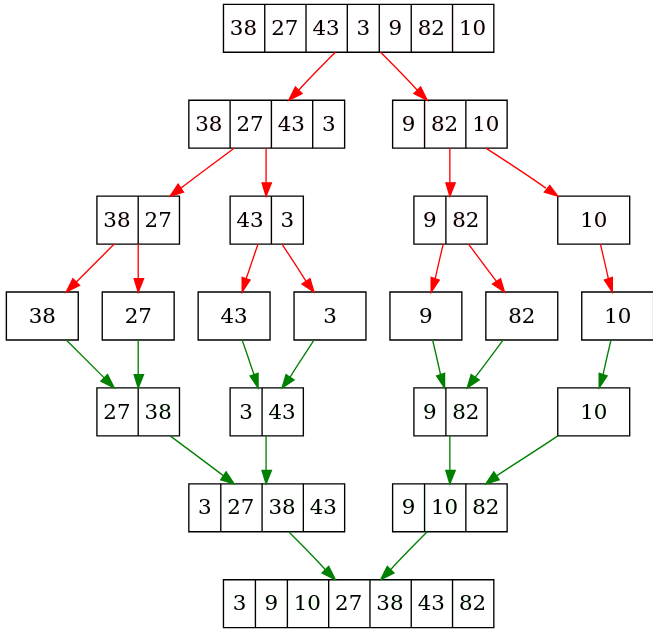
\includegraphics[width=200pt,height=150pt]{slike/mege.png} %merge-sort-example.png}
 	\label{fig:merge-sort}
 	\caption{Sortiranje spajanjem pomoću podijeli pa zavladaj paradigme: korak po korak}
 \end{figure}

\begin{example}

\textbf{\textit{Množenje cijelih brojeva}}. Za  množenje dva $n$-cifrena broja, metodom koji se uči u nižim razredima osnovne škole, množeći cifru po cifru, zahtijeva se vrijeme izvršavanja od $O(n^2)$.  Konstruisati algoritam zasnovan na paradigmi podijeli pa zavladaj za problem množenja dva broja. 
\end{example}
\begin{solution}
 
 
 Jednostavnosti radi, smatramo da su u ulazu binarni brojevi sa istim brojem cifara.
Pokušajmo sa alternativnom metodom koja će voditi paradigmi podijeli pa vladaj.  Napišimo svaki od brojeva u obliku: $x= x_1 2^{n/2} + x_2, y= y_1 2^{n/2} + y_2$.
Tada je 
$$ xy = (x_1 2^{n/2} + x_2) \cdot (y_1 2^{n/2} + y_2) = x_1 y_1 2^n + (x_1 y_2 + y_1 x_2)2^{n/2} + x_2y_2.$$
Dakle, da bismo izračunali proizvod dva (binarna) broja sa $n$ cifara, treba da izračunamo proizvod $q=4$ broja sa po $n/2$ cifara. Stoga, kompleksnost u ovom slučaju je i dalje $O(n^{\log_2 4}) = O(n^2)$. Da bismo ubrzali algoritam,   uradimo sljedeće operacije u datom redoslijedu:
\begin{itemize}
	\item Izračunajmo $x_1y_1$ i $x_2 y_2$.
	\item Izračunajmo $(x_1 + x_2 ) \cdot (y_1 + y_2) = x_1y_1 + x_1y_2 + x_2 y_1 + x_2 y_2$.
	\item Iz prethodnog izraza izvucimo vrijednost $x_1 y_2 + x_2 y_1$.
\end{itemize}
Iz Master teoreme, slijedi da je sada kompleksnost algoritma jednaka $O(n^{\log_2 3})$.
\end{solution}

\section{Algoritamska paradigma vraćanja unazad }

  \textit{Vraćanje unazad} (\textit{backtracking}) je algoritamska tehnika za rekurzivno rješavanje problema postepenom izgradnjom  rješenja, dio-po-dio, uklanjajući ona (parcijalna) rješenja koja ne zadovoljavaju ograničenja problema, momentalno nakon dodavanja nove komponente koja narušava uslove dopustivosti (odnosi se na vrijeme koje je proteklo do dostizanja bilo kojeg nivoa stabla pretraživanja). Za ovu paradigmu se može reći da je ona  poboljšanje pristupa grube sile.
  
  U osnovi,   traži  se  rješenje problema među svim dostupnim opcijama. U početku krećemo od jedne moguće opcije i ako se problem može riješiti tom opcijom, vraćamo dato rješenje. U suprotnom vraćamo se unazad, birajući drugu opciju među preostalim   opcijama. Slučaj u kojem  niti jedna od opcija ne daje rješenje rezultira scenarijem da se neće naći nikakvo rješenje za  određeni problem.  Vraćanje unazad predstavlja rekurzivni pristup jer se proces pronalaska rješenja iz različitih dostupnih opcija rekurzivno ponavlja, sve dok se ne nađe rješenje problema ili dok se dođe do konačnog stanja.
  
  
   Tehnika vraćanja unazad u svakom koraku eliminiše one izbore koji ne mogu dati rješenje i nastavlja   sa onim izborima koji imaju potencijal da odvedu do rješenja. Algoritmi vraćanja unatrag su generalno eksponencijalni i  vremenski i prostorno te se ne preporučuju za rješavanje teških problema.  
    
    Postavlja se pitanje kako prepoznati da se neki problem može riješiti pomoću ove algoritamske paradigme. Dakle, osnovna ideja je da se rješenja problema mogu konstruisati inkrementalno, dodavanjem jedne kompomente za drugom u svakom koraku u postojeće (parcijalno) rješenje, dok se ne dobije rješenje problema ili ne utvrdi da se tim izborom komponenete, nikada neće dobiti validno rješenje (nakon čega se pretraga vraća nazad, pretražujući druge opcije). Prevedeno na jezik rješavanja podproblema, algoritamska paradigma vraćanja unazad rješava sve podprobleme jedan za drugim, kako bi  došla do najboljeg mogućeg rješenja. 
    
    Pseudokod paradigme varaćanja unazad je dat Algoritmom~\ref{alg:backtrack}. 
    
    \begin{algorithm}
    	\begin{algorithmic}[1]
    		\Procedure{Backtrack}{$x$}
    		   \If{$x$ nije rješenje}
    		        \State return \textbf{false}
    		   \EndIf
    		  \If{$x$ je novo rješenje}
    		     \State dodaj $x$ u listu rješenja
    		  \EndIf
    		 \For{svaku moguću opciju $e$}
    		      \State \textsc{Backtrack}(proširi $x$ sa $e$)
    		  \EndFor
    		\EndProcedure
    	\end{algorithmic}

        \caption{Paradigma vraćanja unazad. }        \label{alg:backtrack}
    \end{algorithm}
    
    Napomenimo da je implementacija ovog algoritma vezana za konstruisanje stabla odluke, koje se češće naziva \textit{stablo stanja} (eng. \textit{state-space tree}). U okviru ovog kursa ne ulazimo u ovu notaciju, nego bez previše formalizma pokušavamo objasniti rad osnovnih algoritamskih paradigmi i način rješavanja problema pomoću svake od njih.    
    
    %https://www.programiz.com/dsa/backtracking-algorithm ==> primjer 1...
    
    \begin{example}
    	\textbf{\emph{Problem N kraljica}}.  Neka je data šahovska ploča dimenzije $N\times N$. Smjestiti $N $ kraljica na šahovsku ploču tako da se nikoje dvije kraljice međusobno ne napadaju.  Korisiti algoritam vraćanja unazad. 
    \end{example}

\begin{solution}
           
      Pogledajmo problem 8 kraljica, te jedno njeno rješenje dato na sljedećoj slici.  
      \begin{figure}[H]
      	\centering
      	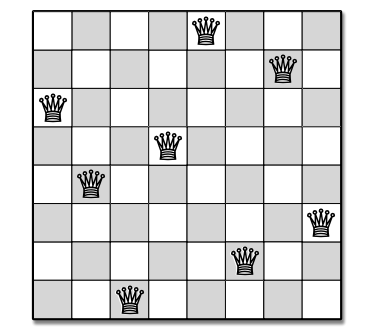
\includegraphics[width=200pt,height=180pt]{slike/n-queen-problem.png}
       \caption{Primjer jednog rješenja problema 8-kraljica.}\label{fig:8-queen-sol-example}
  \end{figure}

Jasno je da se po jedna kraljica smiješta u svakom redu šahovske ploče. Pozicija kraljice u $i$-tom redu je određena brojem kolone u kojoj je ta kraljica postavljena. U prevodu, svako rješenje koje odgovara poziciji kraljica na ploči možemo kodirati nizom \emph{niz} dužine $N$, gdje se na poziciji $i$ nalazi broj kolone u $i$-tom redu u kojoj je smještena kraljica. Konkretno, rješenje (pozicije kraljica)  na prethodnoj slici kodirano je nizom $[5, 7, 1, 4, 2, 8, 6, 3]$. 

Algoritam vraćanja unazad kreće od inicijalno prazne ploče i u svakom koraku nastoji dodati kraljicu u sljedeći (prazni) red. Dakle, kreće se od praznog rješenja, u koji se dodaje novi element   koji odgovara poziciji kraljice sljedećeg (nepopunjenog) reda. Stoga, pri dodavanju nove kraljice u rješenje \emph{niz}, ispitujemo da li pozicije kraljica u (produženom) rješenju  zadovoljavaju uslove zadatka (ne  postoje dvije kraljice koje napadaju jedna drugu). U slučaju da postoji konflikt između nekih kraljica, algoritam se vraća unazad na rješenje \emph{niz} prije dodavanja posljednje dodane kraljice, i razmatra nove pozicije za dodavanje kraljice u tom redu -- tj. za proširivanje trenutnog rješenja.  Ovaj proces se ponavlja sve dok se ne nađe prvo rješenje dužine $N$ koje zadovoljava uslove zadatka (tj. popune se svi redovi na ploči sa kraljicama koje se međusobno ne napadaju), ili se ustanovi da takvo rješenje ne postoji. 

   
Implementacija u Pajtonu koja rješava ovaj problem je data narednim k\^odom. 

\begin{minted}[fontsize=\footnotesize,scale=0.8]{python}
	
   def NQueens(niz, N):
       if len(niz) == N: # kompletno rješenje
               return niz
       else:
              for i in range(N):
                  niz = niz + [i]
                  if not valid(niz): #backtrack ako nije 
                     NQueens(niz + [i])

N = 8
sol = NQueens([], N)       
if sol != None:
   print("Rješenje je: ", sol)
else:
   print("Nema rješenja") #npr. za N=3
   
\end{minted}
%%https://codeahoy.com/learn/recursion/ch10/
\begin{figure}
	\centering
	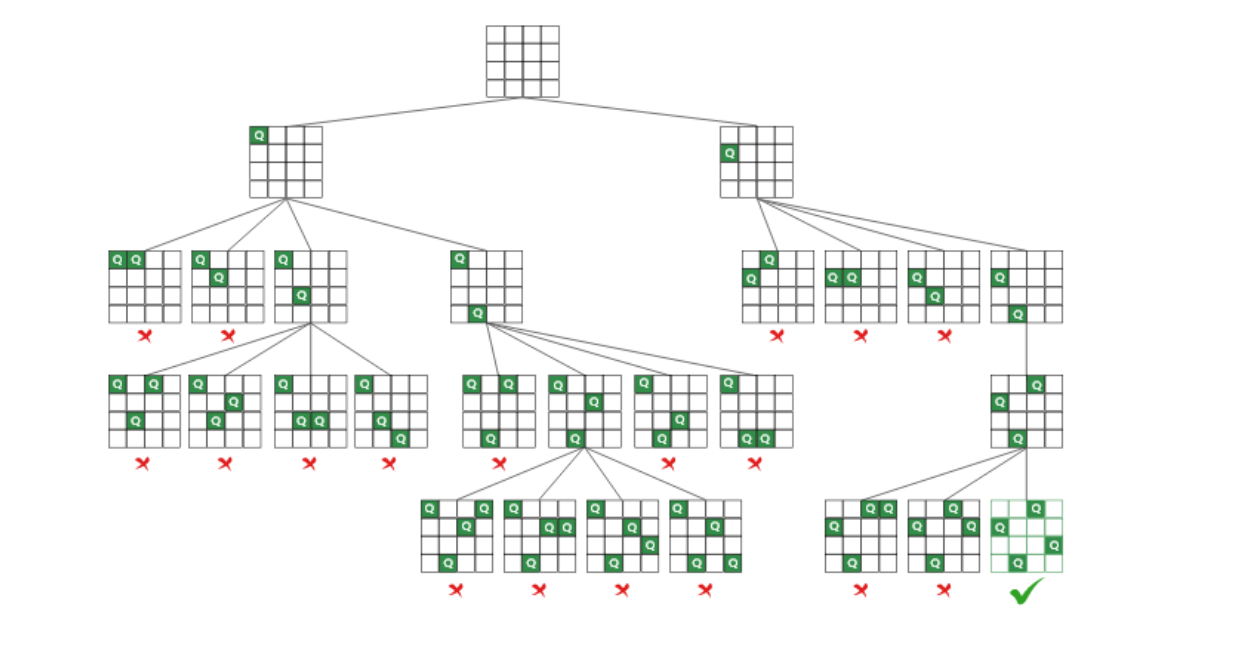
\includegraphics[width=450pt, height=300pt]{slike/n-queen-backtracking.png} %recursion-tree-backtracking-n-queens-1.png}
	\caption{Primjer stabla stanja formiranog algoritmom vraćanja unazad za problem 4 kraljice.}
\end{figure}
%\protect\footnotemark\footnotetext{Slika sa linka \url{https://towardsdatascience.com/genetic-algorithm-vs-backtracking-n-queen-problem-cdf38e15d73f}}

Napomenimo da ovdje nismo prikazali implementaciju funkcije \textit{valid}(), koja vraća \textit{True} ako je pozicija kraljica  validna, u protivnom vraća \textit{False}. Ovo ostavljamo čitaocu kao zadatak za vježbanje. 


\end{solution}


    
 % Što se tiče problema koje ova paradigma rješava, dijelimo ih na tri tipa:
  %\begin{itemize}
  %	\item   \textit{Problem odlučivanja} -- U ovom slučaju tražimo izvodljivo rješenje.
  %	\item   \textit{Problem optimizacije} – U ovome tražimo najbolje rješenje.
  %	\item   \textit{Problem enumeracije} – U ovome nalazimo sva izvodljiva rješenja.
  %\end{itemize}


%https://codeahoy.com/learn/recursion/ch11/: THE SUM OF 4 SQUARES:

\begin{example}
	\textit{Problem sume 4 kvadrata}. Lagranžova teorema o 4 kvadrata kaže da se svaki prirodni broj može napisati kao zbir četiri broja koji su kvadrati nekih brojeva. Neka je dat broj $n$. Naći četiri kvadratna broja koji u zbiru daju broj $n$ pomoću algoritma vraćanja unazad. \\
	Npr. za $n=2000$, vrijedi $1764 + 196 + 36 + 4 = 2000. $
\end{example}

\begin{solution}
	Rješenje problema predstavlja četvorka $sol = (a, b, c, d)$ prirodnih brojeva, tako da je $a^2 + b^2 + c^2 + d^2 = n$. Ideja rekurzije je odabrati svaki  od brojeva jedan po jedan, dok ne dobijemo četvorku koja odgovara uslovima zadatka. Svaki put kada dodamo novi broj $x$ u rješenje \emph{sol}, naredni rekurivni poziv ispituje trenutno zbir kvadrata brojeva u proširenom rješenju \emph{sol}. Ako ono prelazi $n$, algoritam vrši vraćanje unazad i bira novog kandidata za proširivanje rješenja. 
	
 Implementacija algoritma vraćanja unazad za ovaj problem je dat narednim k\^odom.
 
 \begin{minted}[fontsize=\footnotesize,scale=0.8]{python}
 	  
from math import sqrt, pow

def FourSquareSum(sol):
	sum = 0
	for s in sol:
		sum += pow(s, 2)
	return sum

def FourSumSquares(sol, n):
	if len(sol) == 4:
		if FourSquareSum(sol) == n:
			print(sol)
	else:
		for i in range(1, int(sqrt(n))+2):
			solI = sol + [i]
			sum_sol_i = FourSquareSum(solI)
			if sum_sol_i <= n-(4-len(solI)): # else backtrack  
				FourSumSquares(solI, n) 
# poziv metode
FourSumSquares([], 20)
 \end{minted}
	
	Kao što primijećujemo u prethodnom kodu, ako je \emph{sol} kardinalnosti 4, i ako je zbir kvadrata njegovih elemenata jednak $n$, ispisujemo \emph{sol} kao rješenje. U protivnom, ako je $|sol|<4$, (parcijalno) rješenje \emph{sol} proširujemo ubacujući naredni broj (varijabla $i\in \{1, \ldots, \lfloor\sqrt{n} \rfloor + 1 \}$), dobijajući niz \emph{solI}.  Ako je zbir kvadrata elemenata iz \emph{sol} veći od $n-(4 - |solI|)$, ovakva ekstenzija nikada neće voditi ka rješenju koje zadovoljava uslove zadatka, pa pretraga ide unazad, rekurzivno, provjeravajući druge kandidate za proširenje trenutnog rješenja \emph{sol}. Na početku, rješenje \emph{sol} je predstavljeno prazanim nizom.
	 
\end{solution}
 
 
\section{Pohlepni algoritmi}
 % https://www.programiz.com/dsa/greedy-algorithm
\textit{Pohlepni algoritam} je pristup rješavanju problema odabirom najbolje dostupne opcije u datom trenutku za trenutno rješenje u koristeći neki (pohlepni, intuitivni) kriterijum. Pristup ne brine da li će lokalno najbolji odabir uticati ili ne na optimalni rezultat. Algoritam nikada ne poništava raniju odluku čak i u slučaju da je izbor pogrešan. Upravo zbog toga se ovom algoritamskom paradigmom generalno ne može  garantovati nalazak optimalnog rješenja. Dakle, uvijek se traži najbolji lokalni izbor u nadi da će ta odluka voditi   najboljem globalnom rezultatu. U principu, ova paradigma pripada   pristupu \textit{odozgo prema dolje} (eng. \textit{top-down approach}). 

U neformalnom smislu, pohlepni algoritam je algoritam koji počinje jednostavnim, nekompletnim, tj. parcijalnim rješenjem (teškog) problema, a zatim iterativno traži najbolji način za poboljšanje rješenja proširujući ga iterativno, dok ono ne postane kompletno (neproširivo). Pseudokod ove algoritamske paradigme je dat Algoritmom~\ref{alg:greedy-algorithm}. 

Ulaz u algoritam su problem $\mathcal{P}$, instanca problema, te pohlepna funkcija $g$.  Algoritam kreće od nekog, obično praznog, parcijalnog rješenja koje se kroz iteracije nastoji proširiti najboljim mogućim odlukama (komponentama). U svakoj iteraciji izvršava se sljedeće:
 \begin{itemize}
 	\item Za trenutno rješenje $x$, izračunava se skup komponenti koje na dopustiv način (u odnosu na ograničenja problema $\mathcal{P}$) proširuju $x$;
 	\item Među svim takvim komponentama, bira se ono koje (naizgled) najviše doprinosi kvalitetu krajnjeg rješenja; ova odluka se donosi na osnovu pohepne funkcije $g$, koja se još naziva i \textit{heuristička} funkcija. 
 	\item Proširimo rješenje sa najboljom komponentom rješenja.
 \end{itemize}
Ovaj proces se izvršava sve dok je skup komponenti koje dopustivo proširuju trenutno rješenje neprazan. Nakon prekida, vraćamo dobijeno rješenje.

 %%Proces se ponavlja sve do nekog uslova zaustavljanja.

\begin{algorithm}
	\begin{algorithmic}[1]
		\State \textbf{Ulaz:}   instanca nekog problema $\mathcal{P}$, pohlepna funkcija $g$
		\State \textbf{Izlaz}: (aproksimativno) rješenje instance problema $\mathcal{P}$
		\State $x\gets$ inicijalno parcijalno rješenje problema $\mathcal{P}$
		\State $\mathcal{C}\gets$ odredi komponente rješenja koje dopustivo proširuju rješenje $x$
		\While{$\mathcal{C} \neq \emptyset$}
		    \State $e \gets$ odaberi lokalno najbolju komponentu iz $\mathcal{C}$ u odnosu na pohlepnu funkciju $g$
		    \State Proširi $x$ sa $e$
		     \State $\mathcal{C}\gets$ odredi komponente rješenja u odnosu na prošireno rješenje $x$
		\EndWhile
		%\If{$x$ je dopustivo}
		   \State \textbf{return} $x$
		%\Else
		 %   \State Poruka da (dopustivo) rješenje nije nađeno
		%\EndIf
	\end{algorithmic}

    \caption{Shema paradigme pohlepnih algoritama.}    \label{alg:greedy-algorithm}
\end{algorithm}

Dakle, da bimo primijenili pohlepni pristup u rješavanju problema, potrebno je definisati: ($i$) skup komponenti rješenja; ($ii$) strukturu parcijalnog rješenja; ($ii$) pohlepnu funkciju koja računa kvalitet komponente koja može proširiti postojeće parcijalno rješenje. 



Ovu paradigmu koristimo kada je potrebno dobiti rješenje razumnog kvaliteta   u relativno kratkom vremenskom intervalu, na jeftin način (kodirajući relativno brzo). Ovo je često jedna od prvih tehnika koja se primijenjuje u rješavanju teških 
problema.  Ovi algoritmi se takođe koriste u svrhu dobijanja početnog rješenja koje se zatim  poboljšava naprednijim tehnikama. U osnovi, ova paradigma nam nudi dobru polaznu osnovu da ``opipamo'' problem, da se osjeti  koliko je on težak, te da se dobije na uvid koliko heurističke, konstruktibilne (aproksimativne) metode mogu biti efikasne za rješavanje takvih problema.

U nastavku navodimo nekoliko primjena pohelpnih algoritama u rješavanju raznih tipova (kombinatornih) problema. 



\begin{example}\textbf{Problem razmjenjivanja novca}. 
 Imamo  $X$ KM-ova. Na rapolaganju su apoeni od $x_1, x_2, \ldots , x_k$ KM-ova, negoraničene količine. Pretpostavimo da su $X, x_i, i=1,\ldots, n$ prirodni brojevi.

Na koji način razmijeniti $X$ KM-ova tako da se dobije što manji broj
novčanica? Rješiti zadatak pomoću paradigme pohlepnih algoritama.
\end{example}

\begin{solution}
	 Definišimo rješenje problema i njegovu strukturu. Bilo koja $k$-torka $(p_1, p_2, \ldots , p_k )$, gdje je $p_i$ broj
	 apoena novčanice od $x_i$ KM-ova tako da je $\sum_i p_i = X$
	 (razmjenjena je količina od $X$ KM-ova) prestavlja (dopustivo) rješenje. 
	 Parcijalno rješenje problema je bilo koja $s$-torka $(p_1, p_2, \ldots , p_s )$ za koju je $\sum_i^s p_i \leq X, s \leq k$.  Ovakvo rješenje se može nadopuniti do dopustovog. \\ 
	 
	 Konstruišimo sada pohlepnu funkciju. Ideja je da prvo razmatramo novčanice najvećeg mogućeg apoena koji je manji od $X$. Uzmimo  koliko možemo takvih novčanica, ali da se ne premaši ukupna vrijednost od $X$. Od preostalog iznosa $X'$ koji treba da bude razmijenjen, uzmemo onoliko novčanica maksimalne vrijednosti apoena, koja je manji od $X'$, u količini koliko god je to  moguće. Ovaj proces nastavimo, dok ne dobijemo dopustivo rješenje. 
	 
	 Prema tome, prvo sortiramo vrijednosti apoena od najvećeg do najmanjeg. Pretpostavimo bez smanjenja opštosti da je  početni redoslijed apoena $x_1, \ldots, x_k$ dat u sortiranom poretku. Pohlepna funkcija od trenutnog parcijalnog rješenja $s_{partial}=(p_1, \ldots, p_s), s \leq k$ nalazi najmanji indeks apoena $i$ koji je veći od $s$, a da je pri tome $x_i \leq X'= X - \sum_i^s p_i x_i$. Tada je novo prošireno parcijalno rješenje jednako 
	 $$s'_{partial}=(p_1, \ldots, p_s,\underbrace{0,\ldots, 0}_{*}, \underbrace{\lfloor X'/x_i \rfloor}_{p_i} ).$$ 
	 Algoritam se zaustavlja ili kada razmotrimo sve apoene, ili prije toga, kada algoritam nađe (odgovarajuće) rješenje. Implementacija algoritma ovog problema  je data u nastavku.
	 \begin{minted}[fontsize=\footnotesize,scale=0.8]{python}
	 def razmijeni(P, X):
	 	rjesenje = []
	 	i = 0
	 	usitnjeno = 0
	 	brojNovcanica = 0
	 	sortApoeni = sort(P) # sort apoene opadajuće
	 	while i <  n and usitnjeno < X :
	 		pi = (X - usitnjeno) // P[i]  #br. novcanica sortApoeni[i]
	 		if pi > 0:
	 			usitnjeno = usitnjeno + pi * sortApoeni[i]
	 			brojNovcanica = brojNovcanica + pi
	 		i = i + 1
	 	if usitnjeno == X:
	 		return brojNovcanica
	 	else:
	 		return -1 # ne može se usitniti
	 \end{minted} 
\end{solution}

\textit{Kompleksnost algoritma}. Sortiranje algoritma zahtjeva vrijeme od $O(n \log n)$. Dalje, glavna petlja se izvršava u $O(n)$ vremenu, odakle slijedi da je ukupno vrijeme izvršavanja algoritma jednako $O(n \log n)$, što je, svakako, polinomijalno.  Naopmenimo da ovakvom strategijom garantujemo nalazak optimalnog rješenja problema (ili utvrđujemo da rješenje ne postoji). 


\begin{example} \textbf{Razlomljeni problem ruksaka}. 
  Ovaj problem predstavlja relaksiranu verziju problema ruksaka, obrađen u prethodnim sekcijama. Odluka da li uzeti (cio)  proizvod ili ne i staviti u ruksak se relaksira na to da se bilo koji (razlomljeni) dio tog proizoda može uzeti i staviti u ruksak. Zamislimo da je u pitanju proizvod kao što je šećer ili ulje koji (teorijski) može da se dijeli na bilo koji razlomljeni  (realni) dio.  \\
  
   Zadatak je odabrati proizvode (dijelove proizvoda) i staviti u ruksak, tako da je profit maksimalan, ali da se poštuje ograničenje za kapacitet  ruksaka. Koristiti paradigmu pohlepnih algoritama. 
\end{example}

\begin{solution}
	Posmatrajmo primjer instance: $$n = 3, w = [10, 20, 30], p = [60, 100, 120],$$  a 
	kapacitet $C = 50$.  Rješenje ove konkretne instance je uzeti prvi i drugi proizvod u potpunosti (svih 10 i
	20(kg)), dok uzimamo 2/3 trećeg proizvoda (20). Kapacitet ruksaka je zadovoljen,
	a vrijednost proizvoda u ruksaku je jednaka $60 + 100 + 2/3 \cdot  120
	= 240$. \\
	
    \textit{Rješenje i struktura problema}.  Rješenje $c = \{c_1,\ldots, c_n\}$, gdje je $0 \leq c_i \leq 1$ dio uzetog
    proizvoda $i$ koji je stavljen u ruksak, a pri tome je zadovoljen  uslov o poštovanju kapaciteta ruksaka u vrijednosti   $C$.
    
    \textit{Parcijalno rješenje i komponente rješenja}. Parcijalno rješenje je datu o obliku $c = \{ c_{i_1}, \ldots, c_{i_k}  \}$, pri čemu je $i_s \in [n],  i_s \neq i_r, s\neq r,   k \leq n$, a kapacitet ruksaka je zadovoljen. 
    Komponente rješenje u odnosu na parcijalno rješenje $s$ su svi oni proizvodi $C_s = [n] \setminus \{  {i_1}, \ldots, {i_k} \}$ koji se trenutno ne nalaze   u ruksaku. Proširenje parcijalnog rješenja podrazumijeva operaciju dodavanja  količine $c_r>0$ onog proizvoda $r \in C_s$, tako da proširivanjem rješenja $c$ ovom komponentom ne narušavamo kapacitet ruksaka. 
    
    \textit{Pohlepna funkcija}.  Razmotrimo sljedeću razumnu strategiju. Favorizujmo proizvode koji imaju veću cijenu po (jednici) težine, tj. kojima je količnik  $\frac{p_i}{w_i}$ veći u odnosu na ostale. Sortirajmo proizvode po ovom kriterijumu. Neka je, bez smanjenja opštosti, sortirani redosljed proizvoda po ovom kriterijumu dat sa (indeksima) $1,2, \ldots, n$.   \\
    
    
    Dodajmo dio $c_1$ proizvoda indekiranim sa $1$ koliko god je to moguće (maksimalno 1) u odnosu na kapacitet ruksaka. Ako je  $c_1 = 0$, to znači da je kapacitet ruksaka zadovoljen, pretraga se završava. Inače, nastavimo istom strategijom, ažurirajući preostalo stanje ruksaka koji treba da se popuni, a zatim posmatrajući naredni proizvod (sa indeksom 2). Potom određujemo maksimalni udio proizvoda $c_2\geq 0$ koji   (dopustivo) proširuje trenutno  parcijalno rješenje, itd. Petpostavimo da smo istom strategijom generisali rješenje $c = \{ c_{1}, \ldots, c_{k}\}$. %, i_1< \ldots < i_k$.
     Slično, posmatramo naredni proizvod sa indeksom $i =  k+1$, te izračunamo udio tog proizvoda $c_{i}$ kojeg ćemo ubaciti u ruksak, tj. proširiti rješenje $s$. Ako je $c_i = 0$, pretraga se završava. U protivnom, dodajemo komponentu u trenutno parcijalno rješenje, uz ažuriranje stanja o kapacitetu ruksaka koji je preostao za popunjavanje. Pretraga traje sve dok ne popunimo ruksak ili ne razmotrimo sve proizvode.  
      
   Implementacija algoritma je data naredim k\^odom. 
   
   \begin{minted}[fontsize=\footnotesize,scale=0.8]{python}
  def fraction(i):
  	return P[i]/ W[i]
  
  def fraction_knapsack():
  
  	products = [i for i in range(len(W))] #lsit of prods
  	products.sort(key = fraction, reverse=True)
  	#print(products)
  	current_C = C
  	sol = []
  	parts = []
  
  	for i in products:
  
  		part = min(current_C / W[i], 1)
  		if part > 0:
  			sol.append(i)
  			parts.append(part)
  			current_C -= part * W[i]
  
  		else: # knapsack filled
  			return sol, parts
          return sol, parts
    #instanca: 
    W = [10, 20, 30]
    P = [60, 100, 120]
    C = 50
    sol, parts = fraction_knapsack()
    print(sol, " parts: ", parts)
  
   \end{minted}

\textit{Kompleksnost algoritma}.  Najviše vremena je utrošeno na sortiranje proizvoda, što iznosi $O(n \log n)$ vremena. Dalje, u glavnoj petlji, koja se vrti najviše $n$ puta,  svaka iteracija se izvršava u konstantnom vremenu. Dakle, vrijeme izvršavanja petlje je $O(n)$. Prema tome, algoritam se izvršava u $O(n \log n)$ vremenu.

Napomenimo da ovaj algoritam takođe garantuje nalazak optimalnog rješenja. 
\end{solution}


\begin{example} \textbf{Problem pokrivanja skupa}. Neka je dat skup $X$ i podskup njegove familije podskupova $\mathcal{F} \subseteq P(x)$, pri čemu je
	$\cup_{f \in F} f = X$.
	
	Naći podskup $S \subseteq F$ minimalne kardinalnosti $|S|$, tako da je 
  $\cup_{s \in S} s = X$. Problem riješiti uz pomoć paradigme pohlepnih algoritama. 
	
\end{example}

\begin{solution}
	
	Neka je data instanca problema $X = \{1, 2, 3, 4, 5\},$ te $
	\mathcal{F} = \{\{1, 2, 3\}, \{1, 4\}, \{2, 4, 5\}, \{2, 3\}, \{4, 5\}, \{1, 5\}\}$. 
	Rješenje problema je dato sa $S =$ $ \{\{1, 2, 3\}, \{2, 4, 5\}\}$. Njegova kardinalnost je $|S| = 2$.
	
	Ovaj problem ima konkretnu praktičnu primjenu u odabiru minimalnog broja ljudi u komisiju, a da komisija bude kompetentna u svakoj od (traženih) oblasti. Konstruišimo sada algoritam. \\
\textit{Rješenje i struktura rješenja.} Skup (skupova) $S \subseteq \mathcal{F}$ je rješenje problema ako unijom elemenata svih skupova iz $S$ dobijamo skup $X$. 

\textit{Parcijalno rješenje i komponenta rješenja}. Pod parcijalnim rješenjem ovog problema podrazumijevamo bilo koji (pod)skup $S \subseteq \mathcal{F}$ koji ne mora obavezno zadovoljavati uslov o pokrivanju skupa $X$.  Komponenta rješenja $S$ je bilo koji skup iz $C \in \mathcal{F} \setminus S $, dok proširenje rješenja $S$ komponentom rješenja $C$ podrazumijeva operaciju unije, tj. $S' = S \cup \{ C \} $.

\textit{Pohlepna funkcija}. Neka je $S$ parcijalno rješenje i neka ono pokriva $X_S \subseteq X$ elemenata. Intuitivno, bolja opcija podrazumijeva biranje kompomente rješenja $C$ koja u presjeku sa skupom $X \setminus X_S$ ima više elemanta  nego neki drugi sa manjim takvim brojem. Razlog je taj što nastojimo pokriti što više skupa $X$ u što manjem broju koraka pohlepnog algoritma. U simboličkom zapisu, pohlepna funkcija ima sljedeći oblik
$$ g(S, C) = | C \cap ( X \setminus X_S) |,$$
dok biramo element $C^*$ tako da 
$$ C^* \gets argmax \{ g(s, C') \mid C'\in \mathcal{F} \setminus S\} $$
kao element koji će proširiti parcijalno rješenje $S$ u datoj iteraciji.


Algoritam u svakom koraku bira skup $C^*\in \mathcal{F}$ u odnosu na pohlepnu funkciju $g$  i dodaje ga u parcijalno rješenje dok god   rješenje ne pokrije čitav skup $X$, nakon čega se algoritam prekida. Napomenimo da se umjesto kompletnih skupova koji se čuvaju u rješenju $S$, mogu čuvati pozicije (indeksi) skupova iz $\mathcal{F}$ koji pripadaju rješenju $S$. 

Implementacija algoritma  je data u nastavku sljedećim k\^odom.

\begin{minted}[fontsize=\footnotesize,scale=0.8]{python}
	def g(X_S, C):
		return len((X.difference(X_S)).intersection(C))
	def cover_X():
		X_S = set(())
		S = [] # solution
	
		while(X_S != X):
			C_star = istar = None
			g_best = 0
	
			for i in range(len(F)):# iteration best-next
				if i  not  in S: 
					g_i = g(X_S, F[i])
					if g_best < g_i:
						g_best = g_i
						i_star = i
	
			X_S = X_S.union(F[i_star]) #update cover
			S.append(i_star)
		return  S            
	
	#instanca: 
	X = {1, 2, 3, 4, 5}
	F = [{1, 2, 3}, {1, 4}, {2, 4, 5}, {2, 3}, {4, 5}, {1, 5}]
	sol = []
	C = 50
	sol = cover_X()
	print(sol)
	
\end{minted}

\textit{Kompleksnost algoritma}. Glavna \texttt{while}-petlja se izvršava u najviše $n$ iteracija. Dalje, U unutrašnjoj \texttt{for}-petlji, koja se izvršava  $ |\mathcal{F}|$ puta, najskuplja operacija je pozivanje pohlepne \textit{g} funkcije, koja se izvršava u   najviše linearnom vremenu, tj. pripada $O(n)$. Dakle, kompleksnost čitave \texttt{for} petlje je $O(n \cdot  |\mathcal{F} |)$. Dakle, kompleksnost algoritma je $O(n^2 \cdot  |\mathcal{F} |)$. Prema tome, efikasnost algoritma najviše zavisi od veličine skupa $\mathcal{F}$. 

Napomenimo da ovako dizajniran algoritam ne garantuje nalazak optimalnog rješenja  kao u prethodna dva problema. 


  Uzmimo npr. instancu $X= \{1, 2, 3, 4, 5, 6\}$, te $$\mathcal{F}= \{\{1,2\}, \{3, 4\}, \{4, 5\}, \{3, 6\}, \{5\}, \{6\} \}.$$   
  Prva iteracija u algoritmu će uzeti, recimo, prvi skup $\{1, 2\}$ u parcijalno rješenje. Dalje, naredna iteracija uzima skup $\{3, 4\}$. Nakon toga, bira se $\{4, 5\}$, pa $\{6\}$. Dakle, konačno rješenje je kardinalnosti 4. Međutim, to očigledno nije optimalno rječenje. 
  
  Optimalno rješenje   je veličine 3 i dato je sa $\{ \{1, 2\}, \{3, 6\}, \{4,5\}\}$.  
	 
\end{solution}

\begin{example}  \textbf{\textit{Problem sekvencijalnog raspoređivanja poslova}}. Dat je skup  poslova, gdje svaki posao ima dozvoljeno krajnje
	vrijeme završetka (eng. \textit{deadline}) i odgovarajući profit, ako  posao bude završen 
	prije tog vremena. Pretpostavimo da je za izvršavanje svakog posla  potrebno identično (jedinično)
	vrijeme. Startno vrijeme za izvršavanje svih poslova je isto za sve poslove (pretpostavljamo da kreće od 0). \\
	
	  Maksimizovati ukupni profit, pod ograničenjem da se maksimalno jedan
	posao može izvršiti u svakoj jedinici vremena. Riješiti problem pomoću paradigme pohlepnih algoritma. 
\end{example} 

\begin{solution}
	Posmatrajmo primjer instance problema, data sljedećom tabelom.
\begin{center}
 
 
	\begin{tabular}{ccc }
	 \centering
	Posao (ID) & Krajnji rok (Deadline) & Profit \\ \hline \hline
	$1$	&	4	&	20 \\
	$2$	&	1	&	10\\
	$3$	&	1	&	40\\
	$4$	&	1	&	30\\ \hline
	\end{tabular}
\end{center}

Otimalan odabir poslova u slučaju ove instance je: $\{3, 1\}$, sa profitom od 60. 

Posmatrajmo narednu instancu problema.  
\begin{center}
	
	
	\begin{tabular}{ccc }
		\centering
		Posao (ID) & Krajnji rok (Deadline) & Profit \\ \hline \hline
		$1$	&	2	&	100 \\
		$2$	&	1	&	19\\
		$3$	&	2	&	27\\
		$4$	&	1	&	25\\  
	 $5$	&	3	&	15\\   \hline
	\end{tabular}
\end{center}
	
\end{solution}

Rješenje za ovu instancu je odabir poslova iz skupa $\{3, 1,5 \}$ redom kako su i navedeni. Profit ovog rješenja je 142. 


Prva ideja za rješavanje ovog problema je koristiti potpunu enumeraciju: generisati sve podskupove
skupa poslova te za svaki od njih provjeriti dopustivost i na taj način pratiti  
maksimalni profit. Međutim, razmotrimo  tehniku pohlepnih algoritama.   \\ \vspace{0.2cm}

\textit{Rješenje i struktura rješenja}. Svaki podskup $I_s$ skupa svih poslova $I=\{1,\ldots, n\}$ koji zadovoljava uslove zadatka (da se svi mogu izvršiti u okviru njihovog krajnjeg vremena izvršavanja, te nijedan se ne izvršava paralelno sa drugim),  predstavlja rješenje problema. Dalje, struktura rješenja može da bude predstavljena strukturom podataka koja odgovara skupu. 

\textit{Parcijalno rješenje i njegovo proširenje}.  Parcijalno rješenje je bilo koji podskup skupa poslova koji zadovoljava uslove zadatka. Ostatak poslova, koji može da se doda postojećem skupu poslova, a pri tome da ne naruši uslove zadatka, pripada skupu komponenti rješenja koje proširuju dato (parcijalno) rješenje. 

\textit{Pohlepna funkcija}. Za parcijalno rješenje $I_s$, odabrati komponentu rješenja (posao) $i \in I\setminus I_s$ sa maksimalnim profitom koji proširuje $I_s$ na dopustiv način (uslovi zadatka su ispunjeni). Taj posao se, pri tome, smiješta u prvi slobodan (jedinični) interval u kojem se izvršava. 


\textit{Algoritam}. Sortirajmo poslove u odnosu na njihov profit (opadajuće). Bez smanjenja opštosti, pretpostavimo da su oni dati u poretku $\{1, 2, \ldots, n\}$. U provoj iteraciji dodajemo posao 1 maksimalnog profita u parcijalno rješenje $I_s$, koje je inicijalno prazno.  Dalje, pretpostavimo da smo u $i$-toj iteraciji generisali parcijalno rješenje $I_s$. Tada, u narednoj iteraciji razmatramo posao indeksiran sa $i+1$. Moguća su dva scenarija.

\begin{itemize}
	\item Posao sa indeksom $i+1$ ne može da proširi trenutno parcijalno rješenje $I_s$; u tom slučaju idemo na naredni posao ($i+2$);
	\item Posao sa indeksom $i+1$ može da bude dodan u $I_s$. U tom slučaju, nalazimo prvi slobodan jedinični interval u kojem taj posao može da bude izvršen, u odnosu na već raspoređene poslove u trenutnom rješenju $I_s$.  
\end{itemize} 

Algoritam se izvršava sve dok se ne razmotre svi poslovi, nakon čega se vraća konačno rješenje. Implementacija algoritma je data sljedećim k\^odom. 
 
 \begin{minted}[fontsize=\footnotesize,scale=0.8]{python}
 
 def ProfitSort(i):
 	return Profit[i]
 
 # možemo li dodati i-ti proizvod ili ne (-1) u I_s
 def find_next_interval(I_s_covered, i):
 
 	for index, covered in enumerate(I_s_covered):
 		if index >= Deadline[i]:
 			return -1
 		if covered == False:
 			return index
 	return -1        
 
 def sequnetial_scheduling():
 
 	I_s_covered = [False] *  max(Deadline) 
 	I_s = []
 	#sortiranje jobs u odnosu na Profit (preprocessing):
 	Jobs.sort(key=ProfitSort, reverse=True)

 	for i in Jobs:
 
 		interval = find_next_interval(I_s_covered, i)
 		if interval >= 0: #nadjena (dopustiv) interval:
 			I_s_covered[interval] = True #zauzet
 			I_s.append(i)
 
 	return I_s, sum([ Profit[I_s[i]]  for i in range(len(I_s)) ])
 
 #instanca:
 num_jobs = 5
 Jobs = [i for i in range(num_jobs)]
 Deadline = [2, 1, 2, 1, 3]
 Profit = [100, 19, 27, 25, 15]
 # izvrsavanje algoritma:
 I_s, profit = sequnetial_scheduling()
 print(I_s, " profit: ", profit)
 \end{minted}

\textit{Kompleksnost algoritma}. Soritranje poslova se odvija u $O(n \log n)$. Dalje, glavna \texttt{while}-petlja se sastoji od $n$ iteracija. U svakoj iteraciji, najskuplja operacija je pozivanje funkcije \texttt{find\_next\_interval} koja se izvršava u $O(n)$ vremenskoj kompleksnosti. Prema tome,   glavna petlja se izvršava u $O(n^2)$. Zaključujemo da se algoritam izvršava u $O(n^2)$ vremenu. 

Napomenimo da se može pokazati da ovaj pohlepni algoritam garantuje nalazak optimalnog rješenja.

\section{Dinamičko programiranje} 
%https://www.programiz.com/dsa/dynamic-programming

\textit{Dinamičko programiranje} je algoritamska tehnika koja pomaže u efikasnom rješavanju klase problema koji se mogu podijeliti na podprobleme koji se preklapaju (eng. \textit{overlapping subproblems}) i za koje se može definisati \emph{svojstvo optimalne podstrukture} (eng. \textit{optimal substructure property}). Pod preklapajućim podproblemima podrazumijevamo 
one podprobleme čija se rješenja  potrebna više puta da bi se dobilo rješenje početnog problema. Pod optimalnim svojstvom podstrukture   podrazumijevamo da kombinovanjem optimalnih rješenja podproblema dobijamo  optimalno  rješenja datog problema. 

Ako se bilo koji problem može podijeliti na podprobleme, koji su zatim rekurzivno dijele na manje podprobleme, te ako postoji preklapanje među   njima, rješenja podproblema ima smisla  čuvati (u memoriji) za buduću upotrebu. Ovaj proces se naziva \textit{memoizacija}. Memoizacija poboljšava efikasnost rekurzivnog pristupa na taj način da onemogućuje ponovna  evaluacija  istog podproblema već se to rješenje  jednostavno pročita iz određene strukture podataka (poznata još kao heš struktura).   Međutim, ovaj pristup zahtjeva dodatnu memoriju  koja čuva rješenja podproblema.

Da bismo primijenili dinamičko programiranje u rješavanju određenog problema, potrebno je voditi brigu o sljedećim stvarima.
\begin{itemize}
	\item Raščlaniti problem na manje probleme; to uključuje izgradnju adekvatne \textit{rekurzije}, tj. matematičkog modela rješenja; 
	\item Čuvati rješenja podproblema u pogodno odabranoj strukturi podataka -- \textit{memoizacija} (pristup odozgo).
\end{itemize}
%https://www.geeksforgeeks.org/in
%troduction-to-dynamic-programming-data-structures-and-algorithm-tutorials/
Princip dinamičkog programiranja može se implementirati i pristupom odozdo prema gore (eng. \textit{bottom-up approach}), i tada se naziva \textit{tabuliranje} (eng. \textit{tabulation}). Tabuliranjem čuvamo rezultate podproblema u tabelu, potom koristimo te rezultate za rješavanje većih podproblema dok se ne riješi cijeli problem. Dakle, za razliku od pristupa odozgo prema dole, gdje  rekurzivno formulišemo rješenje problema  u smislu njegovih podproblema,  treba da  preformulišemo problem na način da se prvo riješe podproblemi, a potom koriste izračunata rješenja za nadogradnju i dolazak do rješenja većih podproblema.

%Koristi se najčešće kada problem možemo definisati nizom podproblema u kojem se podproblemi ne preklapaju. 
Tabuliranje se obično implementira iterativno i pogodno je za probleme za koje je skup ulaza velik.

Pogledajmo sljedeće primjere izračunavanja $n$-tog fibonačijevog broja u svrhu razumijevanja razlike između memoizacije i tabuliranja.   

\begin{minted}[fontsize=\footnotesize,scale=0.8]{python}
def fib(n, cache={}):# memoizacija
	if n in cache:
		return cache[n]
	if n == 0:
		return 0
	elif n == 1:
		return 1
	else:
		cache[n] = fib(n-1) + fib(n-2)
		return cache[n]
\end{minted}

\begin{minted}{python}  
def fib(n):#tabuliranje
	if n == 0:
		return 0
	elif n == 1:
		return 1
	else:
		tab = [0] * (n + 1) #init
		tab[0] = 0
		tab[1] = 1
		for i in range(2, n+1):
			tab[i] = tab[i-1] + tab[i-2]
		return tab[n]
\end{minted}
U implementaciji memoizacije koristimo objekat rječnika \textit{cache} za čuvanje rezultata poziva funkcija, a rekurzija se koristi za izračunavanje rezultata.

U implementaciji tabele koristimo niz nazvan \texttt{tab} za čuvanje rezultata podproblema, a koristimo iterativnu implementaciju za izračunavanje rezultata. Obje implementacije vraćaju isti rezultat, ali su zasnovane na drugačijoj implementaciji. %Memoizacija je pristup odozgo prema dolje zasnovana na  rekurziji, dok je tabeliranje pristup odozdo prema gore koji koristi iteraciju. 

Da zaključimo, princip dinamičkog programiranja ima smisla koristiti gdje god prepoznamo da rekurzivni pristup ima ponovljive pozive za iste ulaze, koji se optimizuju uz pomoć ove algoritamske paradigme.

\subsection{Rekurzija vs. Dinamičko programiranje}


Dinamičko programiranje se uglavnom primjenjuje na rekurzivne algoritme.  U  osnovi, velika većina problema optimizacije u rješavanju zahtijeva definisanje rekurzije, dok se za njenu  optimizaciju koristi dinamičko programiranje.

Ne mogu se svi problemi koji koriste rekurziju koristiti i dinamičko programiranje. Osim ako ne postoji prisustvo podproblema koji se preklapaju,  kao u problemu računanja fibonačijevog broja, rekurzija može doći do (jednako efikasnog) rješenja problema pomoću pristupa zavadi pa vladaj. U ovome nalazimo  razlog zašto rekurzivni algoritam koji realizuje  sortiranje spajanjem ne može koristiti dinamičko programiranje, jer se podproblemi ni na koji način ne preklapaju (dijeljenje niza na dva disjunktna podniza).


\subsection{Primjene dinamičkog programiranja}

\begin{example}
	Neka je data kvadratna matrica $A=(a_{ij})$ prirodnih brojeva. Pijun se nalazi u gornjem lijevom uglu. On se može kretati jedno polje dolje ili jedno polje dijagonalno dolje-desno u odnosu na trenutni položaj. 
	
	
	Na koji način izabrati putanju hoda pijuna po ploči, od početnog položaja do (bilo koje pozicije) donjeg reda tako da suma brojeva na putu bude maksimalna.
\end{example}

\begin{solution}
	Posmatrajmo jedan primjer validnog puta pijuna na slici~\ref{fig:pijun-putanja}. 
	
	
	\begin{figure}
		\centering
		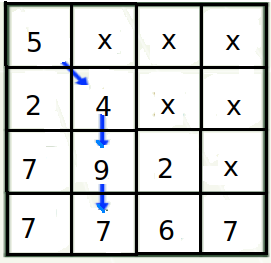
\includegraphics[width=100pt,height=100pt]{slike/dp-table-1.png}
		\caption{Primjer putanje pijuna. Ukupna težina označenog puta je 25.} \label{fig:pijun-putanja}
	\end{figure}

Memoizaciju izvršavamo matricom $M$: na polju $(i , j)$ pamtimo
vrijednost najboljeg puta od pozicije $(0, 0)$ (gornji lijevi ugao) do pozicije $(i , j)$. Pokušajmo   rekurzivno odrediti vrijednost $A(i,j)$ u zavisnosti od odgovarajućih podproblema. Moguća su dva scenarija, pijun je  došao iz pozicije $(i-1, j-1)$ u poziciju $(i,j)$ ili iz pozicije $(i-1, j)$ u poziciju $(i, j)$. Prema tome, vrijedi rekurzija: 

\begin{equation}
	A(i,j) = \max\{ A(i-1, j-1) + a_{ij}, A(i-1, j) + a_{ij}   \}.
\end{equation}
Bazni slučajevi rekurzije su dati sa 
\begin{equation}
	A(0, 0) = a_{00}, A(0, j) = 0, j > 1.
\end{equation}
Rješenje problema nalazimo sljedećom formulom:
\begin{equation}
	\max_{j=0, \ldots, n-1}A(n-1, j)
\end{equation}

Implementacija ovog rješenje je data sljedećim k\^odom (pristup odozgo prema dolje).

\begin{minted}[fontsize=\footnotesize,scale=0.8]{python}
	A = None #matrica sa svim -1
	def init(n):
        
            A = [ [-1] * n for _ in range(n)  ]
            A[0][0] = M[0][0] #bazni slučaj
	
	def solve():#tabuliranje
	
	    for i in range(1, len(M)):
	        for j in range(0, i):
	            best = A[i-1][j]  
	            if j>0 and A[i-1][j-1] != -1:
	                best = max(best,  A[i-1][j-1])
	        A[i][j] = best + A[i][j]
	 
 
		return A

	#instanca
	M=[[4, 5, 7, 0],
    	[2, 3, 1, 3],
    	[1, 1, 3, 1],
    	[2, 3, 3, 3]
        ]	
	init(len(A))
	A = solve()
	max_sum_path = 0
	for j in range(len(M)):
		max_sum_path = max(max_sum_path, A[len(A)-1, j])
		
	print(max_sum_path)
\end{minted}

\textit{Kompleksnost algoritma}. Funkcija \textit{solve} se izvršava u $O(n^2)$ vremenskoj kompleksnosti kao najzahtjevniji dio implementacije. Prema tome, ukupna kompleksnost algoritma je $O(n^2)$.

\end{solution}



\begin{example}
	Riješiti problem ruksaka pomoću dinamičkog programiranja. 
\end{example}

\begin{solution}
	\\
	\textit{Podproblemi}. Riješimo problem ruksaka kapaciteta $j\leq C$ birajući prvih $i\leq n$ proizvoda, tj. one proizvode indekirane sa indeksima $1, \ldots , i$.  Memorišimo rješenje matricom $DP$, konkretno sa $DP[i ][j]$. Dakle, podproblem je definisan parom brojeva $(i,j), i\in \{0, 1, \ldots, n\}, j \in \{0, \ldots, C \}$. 
	
	\textit{Rekurzija}. Posmatrajmo fiksirani podproblem dat parom indeksa $(i, j)$ i nađimo  (manje) podprobleme koji su relevantni za rješavanje njega samog. Vrijedi:
	
	\begin{itemize}
		\item Ako $i$-ti proizvod ne učestvuje u (optimalnom) rješenju podproblema $(i, j)$, tada je jednostavno $DP[i][j] = DP[i-1][j]  $
		\item     Inače, posmatrajmo podprobleme koji uzimaju u razmatranje prvih $k\in \{1, \ldots, i-1\}$ proizvoda. Prvo, podproblemi kojima je kapacitet veći od $C$ nisu relevantni za rješavanje podproblema $(i,j)$. Posmatrajmo neki podproblem $(k,l), k < i, 0 \leq l < j$. Ako možemo dopustivo dodati $i$-ti proizvod u rješenje ovog podproblema, dobijamo potencijalo rješenje većeg podproblema $(i,j)$. Dakle, ako je $l + w_i \leq j$, potencijalno rješenje podproblema je dato sa vrijednošću $D[k][l] + p_i$.  Prema tome, imamo rekurziju:
	   \begin{align*}
		      DP[i ][j ]& = \max\{ D[i-1][j], \max\{DP[k][j - w_i ] + p_i \mid   \\   & j - w_i \geq  0 \ \wedge\  k=1, \ldots, i-1, j \leq C\}\}.
		\end{align*}
	\end{itemize}
	
	 \textit{ Bazni slučajevi}. Ako je kapacitet ruksaka $C=0$, onda je i cijena takvog rješenja jednaka 0, za sve razmatrane proizvode (u ruksak koji ne može da stane ništa, pa ne  stavljamo proizvode). Dakle, $DP[i][0] = 0.$ Takođe, u ruksak bilo kog kapaciteta $j \leq C$, ukoliko ne postoje proizvodi koji se razmatraju za stavljanje u ruksak, pa je trivijalno $DP[0][j] = 0, 0 \leq j \leq C$.
	 
	 Rješenje proizvoda se memoriše u strukturi $DP$ na poziciji indeksa $(n, C)$.
	 
	 Implementacija paradigme dinamičkog programiranja za rješavanje problema ruksaka je data narednim k\^odom.
	 
	 \begin{minted}[fontsize=\footnotesize,scale=0.8]{python}
	 def knapsack(n, C, W, p):
	 	DP = [[0 for x in range(C + 1)] for x in range(n + 1)]
	 
	 	# tabuliranje
	 	for i in range(n + 1):
	 		for j in range(C + 1):
	 			if i == 0 or j == 0:
	 				DP[i][j] = 0
	 			elif W[i-1] <= j:
	 				DP[i][j] = max(p[i-1]
	 				         + DP[i-1][j-W[i-1]],
	 				         DP[i-1][j])
	 			else:
	 				DP[i][j] = DP[i-1][j]
	 
	 	return DP[n][C]
	 
	 #instanca:
	 p = [60, 100, 120]
	 W = [10, 20, 30]
	 C = 50
	 n = len(profit)
	 #poziv funkcije
	 print knapSack(n, C, W, p, n)
	 \end{minted}
	 
 \textit{Kompleksnost algoritma}. Najskuplji dio algoritma su dvije ugnježdene \texttt{for} petlje, koje izvršavaju $O(n \cdot C)$ iteracija. Svaka od iteracija se izvršava u konstantnom vremenu, pa je i ukupna kompleksnost algoritma jednaka $O(n \cdot C)$.
\end{solution}

Navedimo primjer jedne instance i $DP$ tabelu koja se kreira rekurzivno. 

Neka je $n = 4$, te neka je kapacitet ruksaka $C= 5$, dok je  $W = (2, 3, 4, 5)$, a $P = (3, 4, 5, 6)$. 
 %https://codecrucks.com/knapsack-problem-using-dynamic-programming/
 U prvom koraku ($i=0$ i $j =0$) se popunjavaju nule u prvoj vrsti i prvoj koloni matrice $DP$, kako je prikazano u sljedećoj tabeli:
  \begin{table}[H]
 	\centering
 	\begin{tabular}{|c|cc|cccccc|}\hline
 
  	$j\rightarrow$     & Proizvod   &              &	 	0	&1&	2	&3	&4	&5 \\ \hline
        
 $i=0$ & 	& 	    & 	        0	&0	&0	&0	&0	&0  \\
 $i=1$ &	$w_1=2$	&$p_1=3$ &	0	& 	& 	& 	& 	&\\ 
 $i=2$ &	$w_2=3$	&$p_2=4$ &	0   &	& 	& 	&	&\\	 
 $i=3$ &	$w_3=4$	&$p_3=5$ &	0	& 	& 	& 	& 	&\\ 
 $i=4$ &	$w_4=5$ &$p_4=6$ &	0	& 	& 	& 	& 	&\\ \hline
 \end{tabular}
\end{table}
 
 Dalje, za $i = 1$, imao sljedeće izračunavanje: 
 \begin{itemize}
 	\item proizvod 1 ima težinu 2 i vrijednost 3, pa u drugoj vrsti matrice $DP$ ($i=1$) sve do trećeg elementa ($j=2$) vrijednosti su 0, dok je krenuvši sa tim elementom, svakoj poziciji dodijeljena vrijednost 3 (=$p_1$). 
 \end{itemize}
Dakle, popunjavamo drugu vrstu kao u sljedećoj tabeli:
 
   \begin{table}[H]
 	\centering
 	\begin{tabular}{|c|cc|cccccc|}\hline
 		
 	$j\rightarrow$	& Proizvod   &              &	 	0	&1&	2	&3	&4	&5 \\ \hline
 		
 		$i=0$ & 	& 	    & 	    0	&0	&0	&0	&0	&0  \\
 		$i=1$ &	$w_1=2$	&$p_1=3$ &	0	&0 	&3 	&3 	&3 	&3\\ 
 		$i=2$ &	$w_2=3$	&$p_2=4$ &	0   &	& 	& 	&	&\\	 
 		$i=3$ &	$w_3=4$	&$p_3=5$ &	0	& 	& 	& 	& 	&\\ 
 		$i=4$ &	$w_4=5$ &$p_4=6$ &	0	& 	& 	& 	& 	&\\ \hline
 	\end{tabular}
 \end{table}
  
  Dalje, za treću vrstu ($i=2$) imamo sljedeću tabelu: 
  
   
  \begin{table}[H]
  	\centering
  	\begin{tabular}{|c|cc|cccccc|}\hline
  		
  		$j\rightarrow$	& Proizvod   &              &	 	0	&1&	2	&3	&4	&5 \\ \hline
  		
  		$i=0$ & 	& 	    & 	    0	&0	&0	&0	&0	&0  \\
  		$i=1$ &	$w_1=2$	&$p_1=3$ &	0	&0 	&3 	&3 	&3 	&3\\ 
  		$i=2$ &	$w_2=3$	&$p_2=4$ &	0   &0	&3 	&4 	&4	&7\\	 
  		$i=3$ &	$w_3=4$	&$p_3=5$ &	0	& 	& 	& 	& 	&\\ 
  		$i=4$ &	$w_4=5$ &$p_4=6$ &	0	& 	& 	& 	& 	&\\ \hline
  	\end{tabular}
  \end{table}
Diskutujmo slučaj $DP[2][4]=4$. Ako rješenje podproblema ne uzima proizvod 2, $DP[1][4]=3$ je potencijalno rješenje. U protivnom, ako se uzme, moguće rješenje razmatranog problema je $4 + DP[2][4-4] = 4 + 0 = 4$. Kako je $\max\{3, 4\}= 4$, slijedi da je $DP[2][4] = 4$.


  Narednom iteracijom, popunjavamo četvrtu vrstu ($i=3$) u prethodnoj tabeli, pa imamo: 

  \begin{table}[H]
	\centering
	\begin{tabular}{|c|cc|cccccc|}\hline
		
		$j\rightarrow$	& Proizvod   &              &	 	0	&1&	2	&3	&4	&5 \\ \hline
		
		$i=0$ & 	& 	    & 	    0	&0	&0	&0	&0	&0  \\
		$i=1$ &	$w_1=2$	&$p_1=3$ &	0	&0 	&3 	&3 	&3 	&3\\ 
		$i=2$ &	$w_2=3$	&$p_2=4$ &	0   &0	&3 	&4 	&4	&7\\	 
		$i=3$ &	$w_3=4$	&$p_3=5$ &	0	&0 	&3 	&4 	&5 	&7 \\ 
		$i=4$ &	$w_4=5$ &$p_4=6$ &	0	& 	& 	& 	& 	&\\ \hline
	\end{tabular}
\end{table}
 Diskutujmo slučaj $DP[3][4]=5$.   Ako rješenje podproblema ne uzima proizvod 3, $DP[2][4]=3 $ je potencijalno rješenje ovog podproblema. Dalje, ako uzima, onda je rješenje $DP[2][4-4] + 5 = 0 + 5 = 5$ potencijalni kandidat za razmatrani podproblem. Kako je $\max\{4, 5\}=5$, slijedi zaključak.
 
   Konačno, posljednjom iteracijom popunjavamo petu vrstu ($i=4$) u prethodnoj tabeli, pa imamo: 
 
 \begin{table}[H]
 	\centering
 	\begin{tabular}{|c|cc|cccccc|}\hline
 		
 		$j\rightarrow$	& Proizvod   &              &	 	0	&1&	2	&3	&4	&5 \\ \hline
 		
 		$i=0$ & 	& 	    & 	    0	&0	&0	&0	&0	&0  \\
 		$i=1$ &	$w_1=2$	&$p_1=3$ &	0	&0 	&3 	&3 	&3 	&3\\ 
 		$i=2$ &	$w_2=3$	&$p_2=4$ &	0   &0	&3 	&4 	&4	&7\\	 
 		$i=3$ &	$w_3=4$	&$p_3=5$ &	0	&0 	&3 	&4 	&5 	&7 \\ 
 		$i=4$ &	$w_4=5$ &$p_4=6$ &	0	&0 	&3 	&4 	&5 	&7\\ \hline
 	\end{tabular}
 \end{table}

 Diskutujmo slučaj $DP[4][5]=7$.  Ako rješenje podproblema ne uzima proizvod 4, $DP[3][5]=7$ je potencijalno rješenje ovog podproblema. Dalje, ako uzima proizvod 4, onda  je i rješenje $DP[4][5-5] + 6 = 0 + 6 = 6$ potencijalni kandidat za razmatrani podproblem. Kako je $\max\{6, 7\}=7$, slijedi zaključak.
 
 \begin{definition}
 	String $s$ je podniz stringa $s_1$ akko se $s$ može dobiti brisanjem (nula ili više)
 	karaktera iz stringa $s_1$ a čuvajući poredak ostalih karaktera. \\
 	Npr.  \texttt{acd} je podniz stringa \texttt{abbbcdef}.   
 	
 	Prefiks stringa $s$ dužine $k$ je podstring stringa $s$ koji se sastoji od prvih $k$ karaktera. Npr. prefiks dužine tri stringa \texttt{abbbcdef} je string \texttt{abb}. 
 	
 \end{definition}
 
 \begin{example}
 	\textit{Problem najdužeg zajedničkog podniza} (eng. \textit{the longest common subsequence problem}-- LCSP).  Neka su u ulazu data dva stringa $s_1$ i $s_2$. Naći najduži mogući string $s$ koji je podniz oba ulazna stringa.  \\
 	
 	Za instancu $s_1=$\texttt{aatdccddc} i $s_2=$\texttt{agccddta}, rješenje je string $s=$\texttt{accdd}. 
 	
 \end{example}

\begin{solution}
	    Definišimo podproblem indukovan parom cijelih brojeva $(i,j), 0 \leq i \leq |s_1|, 0 \leq j \leq |s_2|$  za dva stringa: prvi predstavlja  prefiksni string dužine $i$ stringa $s_1$,  a drugi predstavlja prefiks string dužine $j$ stringa $s_2$.  Čuvajmo rješenje ovakog para prefiksnih stringova indukovanog sa $(i,j)$ u matrici $DP$ na poziciji $(i, j)$, tj. $DP[i][j]$.
	    
	    \textit{Rekurzija}. Neka je dat podproblem $(i, j)$. Nađimo strategiju razbijanja problema na manje podprobleme kao i sve podprobleme relevantni za konstrukciju rješenja podproblema $(i, j)$. Posmatrajmo karaktere na pozicijama $i$ i $j$, prvog i drugog ulaznog stringa, redom.  Moguća su dva slučaja.
	    \begin{itemize}
	    	\item $s_1[i-1] = s_2[j-1]$: U ovom slučaju, vrijedi rekurzija $DP[i][j] = 1 + DP[i-1][j-1]$, jer  se optimalno rješenje podproblema $(i-1, j-1)$ tada može proširiti za 1 (karakter $s_1[i-1]$) tako da je novonastalo rješenje optimalno za podproblem $(i,j)$.
	    	\item  $s_1[i-1] \neq s_2[j-1]$: U ovom slučaju, sigurno karakter predstavljen komponentnim parom  $(s_1[i-1]$, $s_2[j-1])$ ne doprinosi optimalnom rješenju podproblema $(i,j)$. Dakle,  za određivanje optimuma podproblema $(i,j)$ relevantna su dva podproblema: $(i-1, j)$ i $(i, j-1)$, nastala izbacivanjem krajnjih karaktera prvo u prvom, pa onda u drugom prefiksu. Duže (optimalno) rješenje ta dva podproblema će činiti i optimalno rješenje za podproblem $(i,j)$. Dakle, u ovom slučaju vrijedi rekurzija:
	    	$$DP[i][j] = \max \{ DP[i-1][j], DP[i][j-1] \} $$ 
	    	
	    \end{itemize}
	    Rješenje problema nalazimo u $DP$ na poziciji $(|s_1|, |s_2|)$. 
	    
	    \textit{Bazni slučajevi}. Ako je jedan od ulaznih strigova prazan, rješenje je jednako 0, tj.  $DPi][0]= 0, 0 \leq i \leq |s_1|,  DP[0][j] = 0, 0 \leq j \leq |s_2|$. 
	    
	 Implementacija paradigme dinamičkog programiranja za rješavanje LCSP je data narednim k\^odom. 
 \begin{minted}[fontsize=\footnotesize,scale=0.8]{python}
	    	
	    	def LCS(s1, s2): #tabuliranje^
	    	      
	    	  if len(s1)==0 or len(s2)==0:
	    	     return 0
	    	     
	    	  DP = [ [0]*(len(s2)+1) for _ in range(len(s1)+1)]
	              for i in range(1, len(s1)+1):
	    	      for j in range(1, len(s2)+1):
	    		     if s1[i] == s2[i]: 
	    		         DP[i][j] = DP[i-1][j-1] + 1:
	    		     else:
	    		         DP[i][j] = max(DP[i-1][j], DP[i][j-1])
	    		          
	    	return DP[len(s1)][len(s2)]        
	    		           
	    	      
	    	#instanca:
	    	s1 = "abcdcdcdaa"
	    	s2 = "abbaabcccddd"
	    	#poziv DP metoda
	    	lcs = LCS(s1, s2)
	    	print("Duzina LCS-a je: ", lcs)     
 \end{minted}
	     Primijetimo da implementacija koristi princip odozdo-nagore.
	     
	     \textit{Kompleksnost algoritma}. Dvije \texttt{for}-petlje  izvršavaju ukupno $O(|s_1|\cdot |s_2|)$ iteracija. Svaka od iteracija se izvršava u konstantnom vremenu, pa je shodno tome ukupno vrijeme izvršavanja algoritma jednako $O(|s_1| \cdot |s_2|)$. Ako je $n = \max\{|s1|, |s2|\}$, dobijamo (kvadratnu) $O(n^2)$ kompleksnost. 
	     
	     %\begin{figure}[H]
	     %	\centering
	     %	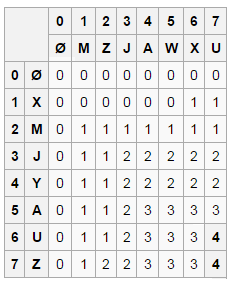
\includegraphics[width=150pt,height=150pt]{slike/dp-lcs-table.png}
	     %	\caption{DP matrica za dva stringa $s_1=$\texttt{MZJAWXU} i $s_2=$\texttt{XMJYAUZ}. Rješenje je dužine 4 (pogledati donji desni ugao matrice). }
	     %\end{figure}
     
     \begin{table}
     	  \centering
     	  \begin{tabular}{cc|cccccccc}
     	  	& & 0&1 &2 &3 &4 &5 &6 &7   \\
     	  
     	  	& & $\emptyset$&\texttt{M} &\texttt{Z} &\texttt{J} &\texttt{A} &\texttt{W} &\texttt{X} &\texttt{U}  \\ \hline \hline
     	  	
     	  	0&$\emptyset$ &0& 0& 0&  0&0 &0 & 0   & 0 	   \\
     	  	1& \texttt{X}& 0& 0& 0& 0& 0& 0&  1  & 1                \\	
     	  	2& \texttt{M}& 0& 1& 1& 1& 1& 1&  1  & 1                \\	
     	  	3& \texttt{J}& 0& 1& 1& 2& 2& 2&  2  & 2                \\	
     	  	4& \texttt{Y}&0 & 1& 1& 2& 2& 2&  2  & 2                 \\	
      	  	5& \texttt{A}& 0& 1& 1& 2& 3& 3&  3  & 3                \\	
      	  	6& \texttt{U}& 0& 1& 1& 2& 3& 3&  3  & 4                \\	
      	  	7& \texttt{Z}& 0& 1& 2& 2& 3& 3&  3  & 4                \\	 \hline \hline
     	  \end{tabular}
 	 \caption{DP matrica za dva stringa $s_1=$\texttt{MZJAWXU} i $s_2=$\texttt{XMJYAUZ}. Rješenje je dužine 4 (pogledati donji desni ugao matrice). }  \label{tab:dp-lcs-example} 
 	\end{table}
\end{solution}

%https://www.programiz.com/dsa/longest-common-subsequence ==> primjer tabele sa rješenjem...

\begin{example}
	\textbf{\textit{Problem sume podskupa}}. Neka je u ulazu dat niz \emph{niz} (od $n$) nenegativnih cijelih brojeva i broj \textit{sum}. 
	
	Da li postoji podniz datog niza \emph{niz} čija je suma elemenata
	  jednaka vrijednosti  \textit{sum}.
\end{example}

\begin{solution}
   Definišimo podproblem indukovan parom $(i, j)$, $0 \leq i \leq n, 0 \leq j \leq sum$ koji razmatra prvih $i$ brojeva niza \emph{niz} i za njih vraća odgovor ($True$ ili $False$) da li se među njima nalaze brojevi čiji je zbir jednak \emph{j}. Čuvajmo rješenje ovakvog podproblema u matrici $DP$, na poziciji $(i,j)$, tj. $DP[i][j]$.  \\ \vspace{0.15cm}
   
   \textit{Rekurzija}. Analizirajmo podprobleme koji su relevantni za rješavanje podproblema $(i,j)$. Razlikujemo dva slučaja:
   \begin{itemize}
   	\item $i$-ti element niza \emph{niz} može biti dio rješenja. Tada se podproblem $(i, j)$ redukuje na podprobleme $(i-1, j-niz[i-1])$ za sve $j$ za koje je  $j-niz[i-1]\geq  0$, dakle %--  i podproblem $(i-1, j)$
   	    $$ DP[i, j] =    DP[i-1][ j- niz[i-1] ]. $$ %DP[i-1, j]\ \vee\
   	\item $i$-ti element niza \emph{niz} nije dio rješenja. Tada se podproblem $(i, j)$ redukuje na podproblem $(i-1, j)$, a rekurzija data sa 
   	$$ DP[i][j] = DP[i-1][j]. $$

   \end{itemize}
   Kombinovanjem ova dva slučaja dobijamo da je
   $$DP[i, j] =   DP[i-1][ j- niz[i-1] ] \vee DP[i-1][j] $$ ako je  $j- niz[i-1]\geq 0$ ili  
     $$DP[i, j] =   DP[i-1][ j- niz[i-1] ] \vee DP[i-1][j],$$ inače. \\
   \textit{Bazni slučajevi}. $DP[i][0] = True, i \geq 0,$ i $DP[0][j] = False,$ za $ j \geq 1$. 
   
    Implementacija paradigme dinamičkog programiranja za rješavanje problema \emph{sume podskupa} je data narednim k\^odom. 
   
   \begin{minted}[fontsize=\footnotesize,scale=0.8]{python}
   	  def sum_array(niz, suma):
   	      #tabulation:
   	      DP = [[False] * (suma +1) for _ in range(len(niz) + 1) ]
   	      for i in range(len(niz)+1):
   	          DP[i][0] = True
   	      
   	      for i in range(1, len(niz)+1):   
   	          for j in range(1, suma+1):
   	              if j >= niz[i-1]:
   	                 DP[i][j] = DP[i-1][j-niz[i-1]] or DP[i-1][j]
   	              else:
   	                 DP[i][j] = DP[i-1][j]
   	  
   	  #instanca:
   	  niz = [3, 34, 4, 12, 5, 2]
   	  suma = 9
   	  postoji = sum_array(niz, suma)
   	  print("Postoji podniz sa sumom" if postoji else  
   	        "Ne postoji podniz sa sumom")
   \end{minted}
\end{solution}
Primijetimo da smo dinamičko programiranje implementirali pomoću pristupa \textit{odozdo prema gore}. 

Implementirajmo sada dinamičko programiranje za ovaj problem pristupom odozgo prema dolje.

   \begin{minted}[fontsize=\footnotesize,scale=0.8]{python}
	def init(niz, sum):
		global DP
		DP = [[-1] * (sum +1) for _ in range(len(niz) + 1) ]
	
	
	def sum_array_top_down(niz, sum, i, j, DP = [ ]):
	
		if DP[i][j] != -1:
			return DP[i][j]
	
		if j == 0:
			DP[i][0] = True
			return True 
		if i == 0: 
			DP[0][j] == False
			return False
		#recursion: 
		if j >= niz[i-1]:
			DP[i][j] = sum_array_top_down(niz, sum, i-1, j, DP) 
	                or sum_array_top_down(niz, sum, i, j-niz[i-1], DP)
			return DP[i][j]
		else:
			DP[i][j] = sum_array_top_down(niz, sum, i-1, j, DP)
			return DP[i][j]
\end{minted}  

\textit{Kompleksnost algoritma}. Broj iteracija koje se izvršavaju je jednak $O(n \cdot sum)$. Svaka iteracija se izvršava u konstantnom vremenu, pa je i ukupna kompleksnost algoritma jednaka  $O(n \cdot sum)$. Dakle, ako je vrijednost \emph{sum} ogromna, ekponencijalno velika u odnosu na veličinu niza, ovakav algoritam će biti neefikasan. 



\begin{example}
	\textbf{\textit{Problem rezanja štapa}}. Dat je štap dužine $n$ i lista cijena štapa dužine $i$, za sve $1 \leq i \leq n$.
	
	Pronaći optimalan način da se isiječe  štap na manje
	štapove da bi se maksimizovao ukupan profit.
\end{example}


\begin{solution}
	Posmatrajmo primjer jedne instance problema: 
	$$ price = [1, 5, 8, 9, 10,
	17, 17, 20].$$  Neka je štap dužine $d=4$.
	Rješenje konkretne instance je rezati štap na dva dijela dužine od po 2. Zarada je u tom slučaju jednaka $5 + 5 = 10$.  \\ \vspace{0.2cm}
	
	 Podprobleme datog problema indukujemo indeksima $i$, $0 \leq i \leq n$, gdje vrijednost indeksa $i$ označava instancu problem rezanja štapa dužine $i$. Pretpostavimo da vrijednost optimalnog rezanja (tj. optimalno rješenje)  instance dužine $i$ čuvamo u nizovnoj strukturi $DP$ na poziciji $i$, tj. $DP[i]$.
	 
	 \textit{Rekurzija}. Podproblem indukovan vrijednošću $i$ možemo  riješiti rješavajući podprobleme koji su indukovani sa $k$, $0 \leq k < i$. To znači da štap dužine $i$ dijelimo na dva dijela, dužine $k$ (sa cijenom $price[k-1]$) $i$ štap dužine $(i-k)$, koji opet razmatramo rekurzivno.  
	 
	 Rekurzija u ovom slučaju izgleda ovako:
	 
	 $$ DP[i] = \max \{ DP[i-k] + price[k-1] \mid 1 \leq k \leq i\}.$$
	 
	 Za bazne slučajeve je $DP[0] = 0$, dok je $DP[1] = price[0]$.
	 Rješenje inicijalnog problema se nalazi u $DP[n]$.
\end{solution}

 Implementacija paradigme dinamičkog programiranja za rješavanje problema  rezanja štapa je data narednim k\^odom. 
 
 \begin{minted}[fontsize=\footnotesize,scale=0.8]{python}
	def stick_cut(d, price):

		DP = [-1] * (d+1)  #init
		DP[0] = 0
		DP[1] = price[0]

		for i in range(2, d+1):
			for k in range(1, i+1):
				if DP[i] < DP[i-k] + price[k-1]: 
					DP[i] =  DP[i-k] + price[k-1]
		return DP[d]       
     
     #instanca
     d = 4
     price = [1, 5, 8, 9, 10, 17, 17, 20] 
     max_profit = stick_cut(d, price)      #poziv:
     print(max_profit)
 \end{minted}

\textit{Kompleksnost algoritma}. Dvije \texttt{for} petlje izvršavaju ukupno najviše $O(d^2)$. Kako se svaka iteracija izvršava u konstantnom vremenu, zaključujemo da je kompleksnost algoritma jednaka $O(d^2)$.

\textit{Napomena}. Pogledajmo drvo koje se kreira algoritmom grube sile na Slici~\ref{fig:brute-force-stick-cut}  pri rješavanju problema rezanja štapa za $d=4$. Ovaj pristup enumeriše sva moguća rješenja za rezanje štapa dužine $d=4$. Prvo uzima cio štap u razmatranje (i njegovu cijenu), zatim otkida dio štapa dužine 1, dok se ostatak štapa (dužine 3) rješava (dijeli) rekurzivno itd. Kompletno rješenje dobijamo sa listovima stabla (označeni sa 0). 
\begin{center}
	\begin{figure}[H]
		\centering
		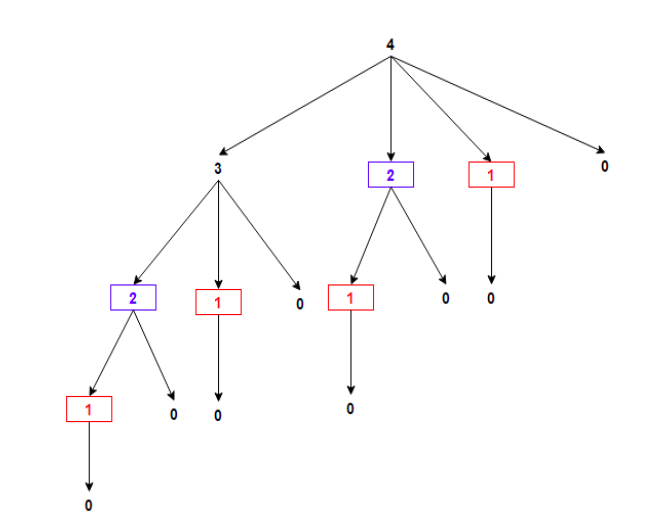
\includegraphics[width=270pt,height=220pt]{slike/brute-force-cutting-stick.png}
		
		\caption{Drvo grananja paradigme grube sile za rješavanje problema rezanja štapa.}\label{fig:brute-force-stick-cut}
	\end{figure}
\end{center}



  Npr. put koji posjećuje čvorove sa oznakama 4 $\rightarrow$ 3 $\rightarrow$ 2 $\rightarrow$ 1 $\rightarrow$ 0, odgovara rješenju u kojem se štap sječe na 4 manja štapa dužine 1 (cijene $4 \times price[0]$). Slično, za put koji posjećuje čvorove sa oznakama 4 $\rightarrow$ 3 $\rightarrow$ 1 $\rightarrow$ 0, odgovara rješenju u kojem se štap sječe na dva manja štapa dužine 1, te jedan dužine 2 (cijene $2 \times price[0] + price[1]$).   
  
   Jasno se vidi da se podproblemi isprepliću, tj. da se, npr. rješavanje problema štapa dužine dva računa više (dva) puta. U slučaju dinamičkog programiranja implementiran  pristupom odozgo prema dolje, stablo će biti značajno redukovano, jer neće postojati rekalkulacije istih podproblema (dakle, nema identičnih kopija podstabala u različitim regionima DP stabla). 
 

\section*{Zadaci}

\begin{enumerate}
	\item Riješiti problem trgovačkog putnika pomoću algoritamske paradigme grube sile.
	\item Riješiti problem ruksaka pomoću algoritamske paradigme grube sile.
	\item Dati  su brojevi  $0 \leq  M  <  N  \leq  1,000,000$. Odrediti  najmanji  broj  sastavljen  samo  od 
	neparnih cifara, koji pri dijeljenju sa $N$ daje ostatak $M$. Ukoliko traženi broj ne postoji, vratiti $−1$. 
	
	 \item Neka su dati prirodni brojevi $n$, koji označava broj promjenljivih, i $s$, koji označava sumu promjenljivih. Uz
pomoć rekurzivnih algoritama napisati program koji pronalazi sva moguća rješenja
za promjenljive  kojih ima $n$ i  čija   suma treba biti jednaka $ s$. 

\textit{Instanca}. $n = 5, s = 4$;
\textit{Rješenje}. 70. \\
\textit{Napomena}:
instanca predstavlja jednačinu $x_1 + x_2 + x_3 + x_4 + x_5 = 4, x_i \in \mathbb{N}$. 
Sva moguća rješenja su:
$(1\ 1\ 1\ 1\ 0), (1\ 0\ 1\ 1\ 1), (0\ 1\ 1\ 1\ 1), \ldots ,$ $(2\ 1\ 0\ 0\ 1), \ldots , (2\ 2\ 0\ 0\ 0)$ itd.
	%pohlepni algoritmi (dva zadatka) 
	%https://www.geeksforgeeks.org/minimum-product-subset-array/
	\item Pronaći podskup elemenata niza tako da je proizvod elemenata u podskupu minimalan. Koristiti paradigmu pohlepnih algoritama.\\
	 \textit{Instanca}. $niz = [ -1, -1, -2, 4, 3]$; \textit{Rješenje}.  -24 ($=(-2 )\cdot (-1) \cdot (-1) \cdot 4 \cdot 3$). 
	
	%https://www.geeksforgeeks.org/greedy-algorithm-egyptian-fraction/
	\item Svaki pozitivan razlomak možemo predstaviti predstaviti kao zbir jedinstvenih jediničnih razlomaka. Razlomak je jedinični razlomak ako je brojnik 1, a nazivnik pozitivan cijeli broj; npr. $1/3$ je jedinični razlomak. Npr. $2/3= 1/2 + 1/6, 3/7=1/3 + 1/11 + 1/231.$   Uz pomoć paradigme pohlepnih algoritama, za proizvoljan razlomak, naći jedinične razlomke koje u zbiru daju taj razlomak.  
	
	
	\item Riješiti problem nalaska najdužeg zajedničkog podniza dva stringa pomoću dinamičkog programiranja pristupom odozgo prema dolje. 
	
	\item Neka je dat niz brojeva u ulazu. Konstruisati algoritam dinamičkog programiranja koji daje odgovor na pitanje li postoji particionisanje niza na dva (disjunktna) skupa tako da je zbir u obje particije jednak.
	\item Implementirati metod dinamičkog progrmairanja  za problem rezanja štapa koristeći pristup odozgo prema dolje.
	
	\item Neka su u ulazu data dva striga $s_1$ i $s_2$. Uz pomoć dinamičkog programiranja, pronaći najkraći string $s$ tako da
	su stringovi $s_1$ i $s_2$ podnizovi stringa $s$.
	\item  Data  je riječ i riječnik (skup riječi). Ispitati da li se riječ može podijeliti na segmente (podstringove) tako da oni pripadaju riječniku. \\
	
	\textit{Instanca}. $$dict = \{\texttt{this}, \texttt{th}, \texttt{is}, \texttt{famous}, \texttt{Word}, \texttt{break}, \texttt{b}, \texttt{r}, \texttt{e}, \texttt{a}, \texttt{k},	\texttt{br}, \texttt{bre}, \texttt{brea}, \texttt{ak}, \texttt{problem} \} $$ te   $$word = \texttt{Wordbreakproblem}.$$  
	\textit{Rješenje}. \texttt{Word break problem},  kao jedno od rješenja.
	
	\item Neka je dat pravougaonik dimenzija $N\times M$. Pretpostavimo da imamo na raspolaganju beskonačan broj pločica
	formata $2^i \times 2^i$, $i = 0, 1, 2, 3, \ldots $. 
	
	Napisati program koji rekurzivno pronalazi minimalan broj pločica koji je potreban da bi se
	popločao pravougaonik datih dimenzija.
	
	\textit{Instanca}.  $N = 6, M=5$;	\textit{Rješenje}. 9 (pločica) -- vidjeti narednu sliku. %~\ref{fig:plocice}. 
	
	\begin{figure}[H]
	    \centering
		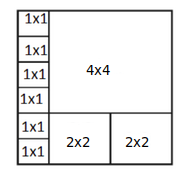
\includegraphics[width=120pt,height=100pt]{slike/plococe-dp-zadatak.png}
		\label{fig:plocice}
		\caption{Optimalno pokrivanje ploče 6 $\times$ 5}
	\end{figure}

\item Napisati program koji generiše sve mogućnosti da se stavi $+$ ili $-$ ili ništa između brojeva $1,2,\ldots,9$ (ovim redom) tako da se kao rezultat izvršenja operacija dobije vrijednost 100. Npr. jedno takvo rješenje je $1 + 2 + 3 - 4 + 5 + 6 + 78 + 9 = 100$.
 
 \item Za dva stringa, napisati program koji ispisuje najkraći niz umetanja i brisanja karaktera u prvi string čijom se primjenom  dobija drugi string.
\end{enumerate}
\chapter{Primjena algoritamskih paradigmi na probleme iz aritmetike}

% https://www.geeksforgeeks.org/dynamic-programming/

U ovoj glavi se bavimo rješavanjem nekih interesantnih problemi iz
aritmetike primijenjujući algoritamske paradigme koje smo obradili u prethodnoj glavi.

\section{Eratostenovo sito}

\begin{definition}
 	Broj $n \in \mathbb{N}$ je \textit{prost} akko je djeljiv isključivo sa 1 i sa samim sobom. 
\end{definition}

Npr. lista prvih 5 prostih brojeva se: 2, 3, 5, 7, i 11. Broj 6 nije prost, jer je djeljiv (pored 1 i 6) sa 2 i sa 3. 

Postavimo sljedeći zadatak. \emph{
Ispitati koliko se prostih brojeva može pronaći,
u nekom razumnom vremenu, među prvih ${N}$ prirodnih brojeva.} \\ 


Paradigmom brutalne sile, ovo bi se moglo riješiti sljedećim rezonovanjem: ispitajmo svaki od (prirodnih) brojeva u intervalu od $2$ do ${N}$ da li je prost ili ne, sljedećom jednostavnom procedurom:

\begin{minted}{python}
     
     def prost(n):
       
       for i in range(2, n):
           if n % i == 0:
              return false
       return True
\end{minted}
Kompleksnost ove procedure je $O(n)=O(N)$ i nju pozivamo $N-1$ puta. Dalje, kompleksnost ovog algoritma bi bila $O(N^2)$. Možemo  li bolje od ovoga? \\

 Iskoristimo ideju da se za neki prost broj $p$, niti jedan od brojeva $k\cdot p, k = 1, \ldots \lceil N/ p \rceil$ nije prost, osim za $k=1$. Dakle, ove brojeve možemo direktno profiltirati iz skupa $\{2, \ldots, N\}$. Zatim, isto se uradi  i za naredni prost broj $p' >p$ u nizu preostalih brojeva, i tako progresivno, sve dok ne dođemo do posljednjeg broja $N$. Dakle, u svakoj iteraciji algoritma, kroz ``sito'' prolaze (filtriraju se) brojevi koji nisu prosti, izvršavajući   provjeru da li je razmatrani broj prost ili ne u konstantnom vremenu. Brojevi koji preostanu u ``situ'' su upravo svi prosti brojevi koji su manji (ili jednaki) $N$.

Implementacija algoritma je data narednim k\^odom. 

\begin{minted}{python}
	def sieve(N):
	   
	   sieve = [True] * (N+1)
	   sieve[0] = sieve [1] = False
	   
	   p = 2
	   while p <= N:
	       
	       if  sieve[p]:
	        
	           index = 2 * p
	           while index <= N:
	               sieve[index] = False
	               index += p
	           
	        p = p + 1
	   
	   for i in range(N+1):
	       if sieve[i]: #broj je prost
	          print(i)
       #poziv funkcije:
       N = 1000
       sieve(N)
\end{minted}  
\textit{Kompleksnost algoritma}.  Može se pokazati da je kompleksnost prethodnog algoritma jednaka $O(N \log\log N )$. 


Demonstrirajmo   prvih nekoliko iteracija ovog algoritma u tabelarnom zapisu, za $N=50.$ 

U početnoj iteraciji, inicira se niz (tabela) brojeva gdje su svi brojevi označeni kao prosti (na poziciji koja odgovara broju se čuva vrijednost \emph{True}).

%\begin{figure}[H]
%	 \centering
%	 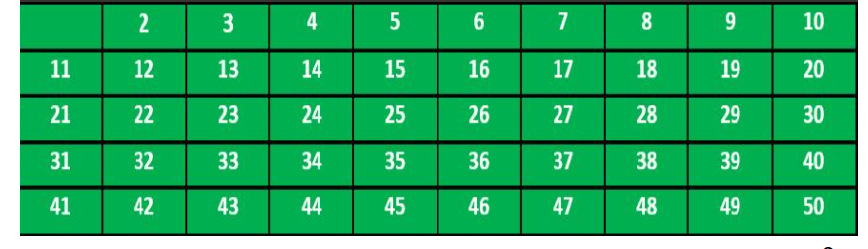
\includegraphics[width=340pt,height=120pt]{slike/sieve-it-0.png}
%\end{figure}

\begin{table}[H]
	\centering
	\begin{tabular}{|c|c|c|c|c|c|c|c|c|c|c} \hline
       & 2 & 3 & 4 & 5 & 6 & 7 & 8 & 9 & 10 \\ \hline
    11 & 12 & 13 & 14 & 15 & 16 & 17 & 18 & 19 & 20 \\ \hline
    21 & 22 & 23 & 24 & 25 & 26 & 27 & 28 & 29 & 30 \\ \hline
    31 & 32 & 33 & 34 & 35 & 36 & 37 & 38 & 39 & 40 \\ \hline
    41 & 42 & 43 & 44 & 45 & 46 & 47 & 48 & 49 & 50 \\ \hline     
	\end{tabular}
    \caption{Inicijalizacija.} \label{eratosten-sieve-it-0}
\end{table}


Dalje, u prvoj iteraciji, nalazimo se na poziciji 2, gdje elemente na pozicijama $2 \cdot k, k=2, \ldots, 50$ eliminišemo kroz sito (kao oni koji nisu prosti, dodijeljujući im vrijednost \emph{False}). Vizuelno, preostali brojevi za ispitivanje su oni neoznačeni:


%\begin{figure}[H]
%	\centering
%	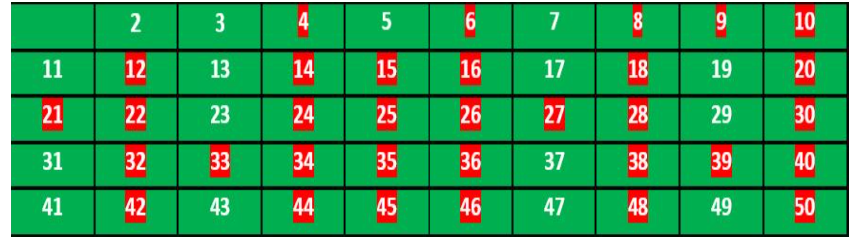
\includegraphics[width=340pt,height=120pt]{slike/sieve-it-1.png}
%\end{figure}

\begin{table}[H]
	\centering
	\begin{tabular}{|c|c|c|c|c|c|c|c|c|c|c} \hline
		& 2 & 3 & \cellcolor{red!30}  4 & 5 & \cellcolor{red!30} 6 & 7 & \cellcolor{red!30} 8 & 9 & \cellcolor{red!30} 10 \\ \hline
		11 &\cellcolor{red!30}  12 & 13 & \cellcolor{red!30} 14 & 15 & \cellcolor{red!30} 16 & 17 & \cellcolor{red!30} \cellcolor{red!30} 18 & 19 & \cellcolor{red!30} \cellcolor{red!30} 20 \\ \hline
		21 & \cellcolor{red!30} 22 & 23 & \cellcolor{red!30} 24 & 25 & \cellcolor{red!30} 26 & 27 &\cellcolor{red!30}  28 & 29 & \cellcolor{red!30} \cellcolor{red!30} 30 \\ \hline
		31 & \cellcolor{red!30} 32 & 33 & \cellcolor{red!30} 34 & 35 & \cellcolor{red!30} 36 & 37 & \cellcolor{red!30} 38 & 39 & \cellcolor{red!30} 40 \\ \hline
		41 & \cellcolor{red!30} 42 & 43 & \cellcolor{red!30} 44 & 45 & \cellcolor{red!30} 46 & 47 &\cellcolor{red!30}  48 & 49 &\cellcolor{red!30}  50 \\ \hline     
	\end{tabular}
        \caption{Eratostenovo sito: iteracija 1.} \label{eratosten-sieve-it-1}
\end{table}



Dalje, u drugoj iteraciji, prelazimo na poziciju 3. Kako je ona označena sa \emph{True} (prost broj), elemente na pozicijama $3\cdot k, k=2, \ldots, 16$ eliminišemo kroz sito (jer nisu prosti). Prelostali brojevi za ispitivanje su oni neoznačeni u narednoj tabeli. 

%\begin{figure}[H]
%	\centering
%	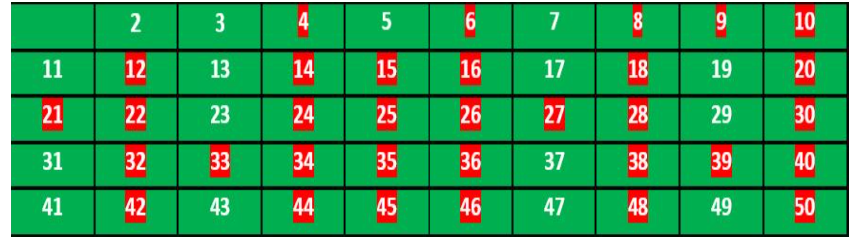
\includegraphics[width=340pt,height=120pt]{slike/sieve-it-1.png}
%\end{figure}

\begin{table}[H]
	\centering
	\begin{tabular}{|c|c|c|c|c|c|c|c|c|c|c} \hline
	& 2 & 3 & \cellcolor{red!30}  4 & 5 & \cellcolor{red!30} 6 & 7 & \cellcolor{red!30} 8 & \cellcolor{red!70} 9 & \cellcolor{red!30} 10 \\ \hline
	11 &\cellcolor{red!30}  12 & 13 & \cellcolor{red!30} 14 & 15 & \cellcolor{red!30} 16 & 17 & \cellcolor{red!30} \cellcolor{red!30} 18 & 19 & \cellcolor{red!30} \cellcolor{red!30} 20 \\ \hline
	21 & \cellcolor{red!30} 22 & 23 & \cellcolor{red!30} 24 & 25 & \cellcolor{red!30} 26 & \cellcolor{red!70}  27 &\cellcolor{red!30}  28 & 29 & \cellcolor{red!30} \cellcolor{red!30} 30 \\ \hline
	31 & \cellcolor{red!30} 32 & 33 & \cellcolor{red!30} 34 & 35 & \cellcolor{red!30} 36 & 37 & \cellcolor{red!30} 38 & 39 & \cellcolor{red!30} 40 \\ \hline
	41 & \cellcolor{red!30} 42 & 43 & \cellcolor{red!30} 44 & 45 & \cellcolor{red!30} 46 & 47 &\cellcolor{red!30}  48 & 49 &\cellcolor{red!30}  50 \\ \hline     
\end{tabular}
        \caption{Eratostenovo sito: iteracija 2.} \label{eratosten-sieve-it-2}
\end{table}

U narednoj iteraciji prelazimo na poziciji 4. Kako to nije prost broj (dakle filtriran prethodno), prelazimo na naredni broj (5), koji je prost, nakon čega ponavljamo operacije opisane prethodnim iteracijama. 


\begin{table}[H]
	\centering
	\begin{tabular}{|c|c|c|c|c|c|c|c|c|c|c} \hline
		& 2 & 3 & \cellcolor{red!30}  4 & 5 & \cellcolor{red!30} 6 & 7 & \cellcolor{red!30} 8 & \cellcolor{red!70} 9 & \cellcolor{red!30} 10 \\ \hline
		11 &\cellcolor{red!30}  12 & 13 & \cellcolor{red!30} 14 & 15 & \cellcolor{red!30} 16 & 17 & \cellcolor{red!30} \cellcolor{red!30} 18 & 19 & \cellcolor{red!30} \cellcolor{red!30} 20 \\ \hline
		21 & \cellcolor{red!30} 22 & 23 & \cellcolor{red!30} 24 & \cellcolor{red!90} 25 & \cellcolor{red!30} 26 & \cellcolor{red!70}  27 &\cellcolor{red!30}  28 & 29 & \cellcolor{red!30} \cellcolor{red!30} 30 \\ \hline
		31 & \cellcolor{red!30} 32 & 33 & \cellcolor{red!30} 34 & 35 & \cellcolor{red!30} 36 & 37 & \cellcolor{red!30} 38 & 39 & \cellcolor{red!30} 40 \\ \hline
		41 & \cellcolor{red!30} 42 & 43 & \cellcolor{red!30} 44 & 45 & \cellcolor{red!30} 46 & 47 &\cellcolor{red!30}  48 & 49 &\cellcolor{red!30}  50 \\ \hline     
	\end{tabular}
	\caption{Eratostenovo sito: iteracija 3.} \label{eratosten-sieve-it-3}
\end{table}

\section{Faktorizacija broja}

Fundamentalna teorema aritmetike nam kaže da se svaki broj $n \in \mathbb{N}$ može na jedinstven način faktorisati na proizvod prostih činilaca, do na redoslijed faktora. Dakle, svaki $n$ se može zapisati u formi
 $$n = \prod_{i=1}^k p_i^{n_i}$$
 za neke $k, n_1,\ldots, n_i, \ldots, n_k \in \mathbb{N}$.
 
 Npr. broj 120 se može faktorisati kao $2^3 \cdot 3^1 \cdot 5^1$.
 
 Sa stanovišta izračunavanja, postavlja se pitanje kako problem izračunavanja faktorizacije broja izvršiti efikasno.  U tu svrhu, iskoristićemo znanje o Eratostenovom situ. 
 
 Prvo primijenimo paradigmu podijeli pa zavladaj. Dake, za broj $n$, nađimo najmanji prost broj $p$ koji dijeli $n$. Tada vrijedi $n = p \cdot n/p$. Dalje, rekurzivno primijenjujemo istu akciju za broj $n/p$ sve dok je $n>1$. Bazni slučaj je kada je broj $n$ prost, i pri tome se kao takav i vraća, prekidajući momentalno rad rekurzije. 
 
 Dakle, potrebno je generisati strukturu podataka  tako da na poziciji $i$ čuva najmanji prost faktor broja $i$; ako je broj prost, čuvamo vrijednost 0.
 
 Implementacija ovakve (nizovne) strukture je data narednim k\^odom. 
 
 \begin{minted}{python}
 
   def sieve_adaptation(n):
   
       sieve_fact = [0] * (n+1)
       sieve_fact[0] = sieve_fact[1] = 0
       p = 2
       while p <= n:
           if sieve_fact[p] == 0:
       		  index = 2 * p
       		  while index <= n:
       			 sieve_fact[index] = p
       			 index += p
           p = p + 1
 	
	return sieve_fact
 	
   def factorization(n):
       
       factorize_min_p = sieve_fact(n)
       F = []
       while True: 
           i = factorize_min_p[n]
           if i == 0: 
              F.append(n)
              return F
           else:
              n = n // i
              F.append(i)
       return F  
   
   #ulaz: 
   n = 120
   F = factorization(n)
   print("Lista faktora je: ", F)
 \end{minted} 
 
\textit{Kompleksnost algoritma}. Najskuplja operacija u algoritmu je adaptacija algoritma Eratostenovog sita (funkcija \texttt{sieve\_adaptation}) i ona se izvršava u $O(n \log \log n)$ vremenu. Glavna \texttt{while}-petlja se izvršava u linearnom $O(n)$ vremenu. Dakle, čitav algoritma se izvršava u 
 $O(n \log \log n)$ vremenu.
 
  \section{Izračunavanje binomnih koeficijenata} 
  
  Binomni koeficijenti igraju bitnu ulogu u kombinatorici. Npr. broj načina na koji se $k$ ljudi može izabrati iz skupa od $n$ ljudi je predstavljen binomnim koeficijentom $\binom{n}{k}$. 
  
  \begin{definition}
  	 Binomni koeficijent $\binom{n}{k}$ gdje je $n, k \in \mathbb{N}, k > 0$  je dat sa 
  	 $$\binom{n}{k} = \frac{n(n-1) \cdots (n-k+1)}{k!}$$
  \end{definition}
  
~ Definišemo $\binom{n}{0} := 1$. Binomni koeficijent $\binom{n}{1} = n,$ dok je $\binom{n}{n} = 1$ za sve $n \in \mathbb{N}.$ Takođe, ako je $n <k$, vrijedi $\binom{n}{k}=0$.
 
  Lako se može pokazati da vrijedi Paskalova jednakost:
  $$ \binom{n}{k} = \binom{n-1}{k-1} + \binom{n-1}{k},$$
   što nam daje rekurziju za računanje binomnih koeficijenta. Dakle, ako označimo $binom(n, k) = \binom{n}{k}$, vrijedi:
   $$ binom(n, k)= binom(n-1, k-1) + binom(n-1, k).$$
   
   Implementacija rekurzivnog pristupa je data sljedećim k\^odom.
   
   \begin{minted}{python}
     def binom(n, k): 
         if k == 0:
            return 1
         if n < k:
            return 0
         return binom(n-1, k-1) + binom(n-1, k)
   \end{minted}
  \textit{Kompleksnost algoritma}. Faktor grananja rekurzije je 2. To znači da na svakoj narednoj dubini rekurzije imamo (najviše) duplo više rekurzivnih poziva nego je to slučaj na dubini prije.  Kako je dubina rekurzije maksimalno $n$ (vrijednost prvog ili drugog atributa se smanjuje za 1 u narednom pozivu rekurzije), zaključujemo da je maksimalni broj poziva rekurzije reda veličine $O(2^n)$, što nam daje eksponencijalnu kompleksnost. \\
  
  Pokušajmo optimizovati ovu naivnu implementaciju rekurzije za računanje binomnih koeficijenata.  Jasno se vidi da se većina podproblema rješava više puta iz nule. Zbog toga upotrebimo princip memoizacije. Struktura u koju čuvamo rješenja je matrica $B[i][j]= \binom{i}{j}$. Bazni slučaj je  dat sa $B(n, 0) = 1 = B(n,n)$. Takođe, ako je $i < j$, imamo $B[i][j] = 0$. Implementacija memoizacije za izračunavanje binomnog koeficijenta $\binom{n}{k}$ je data narednim k\^odom. 
  
  \begin{minted}{python}
  	
  	def initialization(n, k):
  	    Binom = [[-1] * (k+1)  for _ in range(n+1)] 
  	    return Binom 
  	    
  	def binom_memoization(i, j, Binom): 
  	    
  	    if Binom[i][j] != -1: # već računat
  	       return Binom[i][j] 
  	    if j == 0: 
  	       Binom[i][j] = 1
  	       return Binom[i][j] 
  	    if i < j: 
  	       Binom[i][j] = 0 
  	       return Binom[i][j]
  	    Binom[i][j] = binom_memoization(i-1, j-1, Binom) 
  	                + binom_memoization(i-1, j, Binom) 
  	    return Binom[i][j]

    #poziv metode:
    n = 10
    k = 4
    Binom = initialization(n, k) 
    n_over_k = binom_memoization(n, k, Binom) 
    print(n_over_k)
    
  \end{minted}  
  
  \textit{Kompleksnost algoritma}.  Kreiranje strukture se izvršava u $O(n\cdot k)$ vremenskoj kompleksnosti. Dalje,  broj podproblema koji se rješavaju je jednak $(n+1) \cdot (k+1)$.  U svakom rekurzivnom pozivu, izvršava se konstantan broj operacija. Sveukupno, kompleksnost algoritma je jednaka $O(n \cdot k)$. 
  
  
  
   
 \section{Izračunavanje Katalanovih brojeva}
 
 Katalanovi brojevi se pojavljuju u mnogim interesantnim (kombinatornim)
 problemima. Neki od tih problema su sljedeći. 
 
 \begin{itemize}
 	\item Broj različitih puteva sa $2n$ koraka na pravougaonoj mreži $n \times n$ koji polaze od 	donjeg lijevog ugla mreže, tj. koordinate $(n - 1, 0)$, pa do gornjeg desnog ugla $(0, n -1)$ uz dodatan uslov da put ne presijeca glavnu dijagonalu (već je može samo eventualno dodirivati) je predstavljen ovim brojevima.
 	
 	\begin{figure}[H]
 		\centering
 		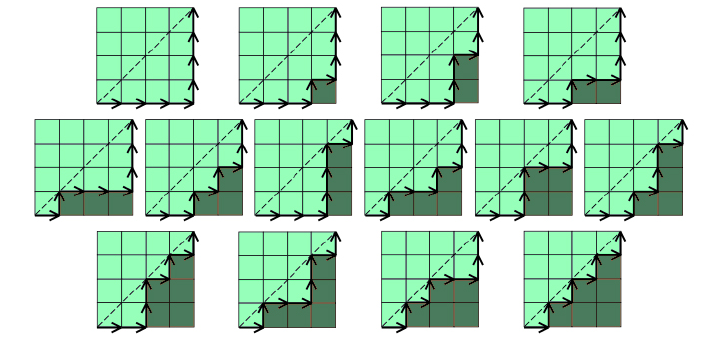
\includegraphics[width=280pt,height=160pt]{slike/catalan-net.png}
 		\caption{Putevi dužine 8 za tablu dimenzija $4\times 4$.} \label{fig:catalan-n-4}
 	\end{figure}
 	\item Broj permutacija skupa $\{1, \ldots, n \}$ koji ne sadrže patern \texttt{123} (ili bilo koji drugi, dužine 3) su predstavljeni Katalanovim brojevima. Npr. za $n = 3$, sljedeće permutacije zadovoljavaju uslove: $132,
 	213, 231, 312$ i $321$.  Dakle, ima ih ukupno 5. 
 \end{itemize}
 
 Prvih nekoliko Katalanovih brojeva su: $1, 1, 2, 5, 14, 42, 132,
 429, 1430, 4862, \ldots $
 
 
 Može se pokazati da za Katalanove brojeve vrijedi sljedeća rekurzija
 
 $$C(0) = 1, C(n+1) = \sum_{i=0}^{n} C(i) \cdot C(n-i), n \geq  0.$$
 
 Primijenimo metod brutalne sile (rekurzivno) pri računanju $n$-tog Katalanovog broja. Implementacija ovog pristupa je data sljedećim k\^odom. 
 
 \begin{minted}{python}
   def catalan(n):
       if n == 0:
          return 1
       catalan_n = 0 
       for i in range(n): 
           catalan_n += catalan(i) * catalan(n-1-i) 
       return catalan_n
        
 \end{minted}
  
  \emph{Kompleksnost algoritma}. Faktor grananja rekurzije je (najviše) $n$. Dubina rekurzije je $n+1$. Dakle, kompleksnost ovog algoritma je ogromna (eksponencijalna) i iznosi $O(n^n)$. 

Pokušajmo optimizovati ovaj (direktni) rekurzivni pristup. Iskoristimo princip memoizacije, zbog toga što se svaki podproblem izražunava iznova više puta. U nizovnoj strukturi $Cat(i)$ čuvajmo vrijednost $i$-tog Katalanovog broja prvi put kada se izračuna.  Vrijedi svojstvo optimalne podstrukture: $Cat(n+1) = \sum_{i=0}^{n} Cat(i) \cdot Cat(n-i).$ Bazni slučaj je dat sa $Cat(0) =1$.

Implementacija memoizacije je data sljedećim k\^odom.

  \begin{minted}{python}
	
	def initialization(n):
	   Cat = [ -1   for _ in range(n+1)  ] 
	   Cat[0]=1
	   return Cat 
	
	def catalan_i(i, Cat): 
	
	    if Cat[i] != -1:
	        return Cat[i]
     
            catalan_i = 0
            for k in range(i): 
                catalan_i += catalan_memoization(k, Cat) *
                     catalan_memoization(i-1-k, Cat)
    
            Cat[i] = catalan_i
            return Cat[i]
    
	   
	#poziv metode:
	n = 10
	Cat = initialization(n) 
	
	cat_n = catalan_n(n, Cat) 
	print(cat_n)
	
\end{minted}  

\emph{Kompleksnost algoritma}. Dubina rekurzije je (najviše) $n+1$. U svakoj rekurziji, broj iteracija koji se izvršava je linearne kompleksnosti $O(n)$. Prema tome, kompleksnost algoritma je $O(n) \cdot O(n) = O(n^2)$. 


 % sretni brojevi, semi-prosti brojevi... 
 
 %Lucky numbers... 
 Posmatrajmo konstrukciju niza brojeva opisanu sljedećom (iterativnom) procedurom.
 
 \begin{itemize}
 	\item Neka je dat niz brojeva:
 	$$1, 2, 3, 4, 5, 6, 7, 8, 9, 10, 11, 12, 13, 14, 15, 16, 17, 18, 19,\ldots $$
 	\item Izbrišemo svaki drugi broj iz skupa, čime dobijamo niz brojeva:
 	$$1, 3, 5, 7, 9, 11, 13, 15, 17, 19,\ldots$$
 	\item Iz prethodnog niza potom izbrišemo svaki treći broj, čime dobijamo novi niz brojeva: $1, 3, 7, 9, 13, 15, 19,\ldots$
 	\item Nastavljamo proceduru brisanja brojeva iz prethodnog niza tako što brišemo svaki četvrti broj u nizu itd.
 \end{itemize} 
 
 U ulazu se zadaje broj $n$. Ispitati da li je on \emph{srećan}, tj. da li neće biti obrisan prethodnom (iterativnom) konstrukcijom. 
 
 \begin{solution}
U prvoj iteraciji ($i=1$) će biti obrisani svi brojevi na parnoj poziciji u nizu, tj. oni koji su djeljivi sa $i+1=2$. Ako $n$ nije djeljiv sa $2$, preživjeće u ovoj iteraciji, te će se u novom (filtriranom) nizu pojaviti na poziciji $\lceil n/2 \rceil$. Dalje, u narednoj iteraciji ($i=2$) provjerimo da li je $\lceil n/2 \rceil < i+1=3$. Ako je to slučaj, broj $n$ nikad neće biti obrisan u narednim iteracijima, pa prekidamo pretragu, vraćajući rezultat \emph{True}. Inače, brišemo sve elemente novog niza čija je pozicija djeljiva sa $3=i+1$. Ako je $\lceil n/2 \rceil$ djeljiv sa 3, $n$ će biti obrisan (prekidamo pretragu, vraćajući rezultat \emph{False}). Inače, broj $n$ preživljava u ovoj iteraciji, te će se nakon operacije brisanja, pojaviti na poziciji $\lceil n/2 \rceil - \lceil n/2 /(i+1)\rceil = \lceil n/(i+1) \rceil = \lceil n/3 \rceil$ novonastalog niza. U narednoj iteraciji ($i=3$), sličnim rezonovanjem prvo provjeravamo da li je $\lceil n/3 \rceil < i+1=4$, pa vraćamo rezultat \emph{True}, ukoliko je to slučaj. Potom, provjeravamo da li je
 $\lceil n/3 \rceil$ djeljiv sa 4. Ako jeste, prekidamo pretragu i vraćamo rezultat \emph{False}. U protivnom, iz trenutnog niza brišemo sve elemente čija je pozicija djeljiva sa $4$, pa će se broj $n$ naći na poziciji $\lceil n/4 \rceil$ novonastalog niza. Ovaj proces ponavljamo, za svaku iteraciju, do prekida (u najgorem slučaju gornja granica broja iteracija je $n$).  
 
 
 Implementacija algoritma je data narednim k\^odom. 
 
 \begin{minted}{python}
 	from math import ceil
 	def lucky_number(n):
 
 	      
 	   for i in range(1, n): #iteracije
 	       if i+1 > ceil(n/i):
 	          return True 
 	       if ceil(n/i)  % (i+1) == 0:
 	          return False
 	   return True       
    
          #poziv funkcije
          print(lucky_number(7)) #True	       
  
 \end{minted}
  
 \end{solution}
 
 \section{Hornerov metod}
 %https://www.geeksforgeeks.org/mathematical-algorithms/
 %https://www.geeksforgeeks.org/horners-method-polynomial-evaluation/
\begin{definition}
	\textbf{\textit{Hornerov metod za računanje vrijednosti polinoma}}. Neka je dat polinom $P(x)=c_n x^n + c_{n-1}x^{n-1} + \cdots + c_1 x + c_0$ kao i tačka $x \in \mathbb{R}$. Naći vrijednost polinoma $P$ u tački $x$. Napomenimo da je ulaz vezan za polinom dat u obliku niza $ coef$ gdje   $coef[i]$ p˙redstavlja koeficijent uz monom  $x^{n-i}$, $i \in \{0, \ldots, n\}$. 

\end{definition}

\begin{solution}
	Pogledajmo primjer sljedeće instance: $coef = [1, -3, 2, -1], x = 3$. U ovom slučaju, riječ je o polinomu $P(x) =  x^3 - 3 x^2 + 2 x -1$. Izlaz    je $ P(3) = 5$.  \\
	
	Naivnim metodom, dakle računanjem vrijednosti $x^n$ običnom petljom se izvršava se u linearnoj $O(n)$ kompleksnosti. Kako imamo $n$ takvih vrijednosti za računanje (koji se potom sabiraju), ukupna kompleksnost ovakvog (naivnog) pristupa je $O(n^2)$.
	
	 Hornerovim metodom, računanje vrijednosti polinoma se može izvršiti u linearnoj $O(n)$ kompleksnosti. Ideju algoritma demonstrirajmo na primjeru polinoma iz prethodnog primjera, koji se može napisati kao:  $$((x - 3)x + 2)x -1.$$ 
	 Dakle, u tom slučaju, evaluacija ovako napisanog polinoma bi išla: prvo krećemo od koeficijenta $c_3=1$ kojeg množimo sa $x=3$ -- pri tome dobijamo (kumulativnu) vrijednost 3. Dalje, trenutnoj vrijednosti   dodajemo vrijednost narednog koeficijenta $c_2 = -3$, te dobijamo vrijednost 0, koju množimo sa $x=3$, dobijajući opet 0. Ponavljamo korak sa narednim koeficijentom $c_1 = 2$, čime dobijamo vrijednost 2, koju množimo sa $x=3$, dobijajući 6. Nadalje, posljednji koeficijent $c_0=-1$ jednostavno dodamo kumulativnoj vrijednosti, odakle dobijamo konačan rezultat, a to je 5. 
	 
	 Gledajući uopšteno, vrijedi: 
	 $$ c_n x^n + c_{n-1}x^{n-1} + \cdots + c_1 x + c_0 = ((\cdots ((c_n x + c_{n-1})x + c_{n-2})x + \cdots c_1) x + c_0  )$$
	 Trivijalni slučaj je  $n=0$, kada je $P(x) = c_0$. U tom slučaju, jednostavno vratimo vrijednost $ c_0$.
	 
	  
	 Implementacija algoritma Hornerovog metoda je data narednim k\^odom. 
	 
	 \begin{minted}{python}
	 	 def horner_metod(coef, n, x):
	 	    
	 	    if n == 0: 
	 	       return coef[0]
	 	    
	 	 	# inicijalizacija
	 	 	res = coef[n]  * x
	 	 	for i in range(1, n):
	 	     	res = res + coef[i]
	 	     	if i < n-1:
	 	     		res *= x
	 	 	return res
	 	 
	 	 # poziv funkcije
	 	 # Evaluacija:  x^3 - 3 x^2 + 2 x -1, x = 3
	 	 coef = [1, -3, 2, -1]
	 	 x = 3
	 	 n = len(coef)
	 	 print(horner_metod(coef, n, x))
	 \end{minted}

\textit{Kompleksnost algoritma.}  Jasno je da je najintenzivniji dio izvršavanja operacija smješten u \texttt{for}-petlju. Svaka iteracija se izvršava u konstantnom vremenu, pa zaključujemo da se algoritam izvršava u linearnom vremenu, tj. $O(n)$.  
\end{solution}
 
 %https://www.geeksforgeeks.org/sieve-of-atkin/ ==> SIEVE OF ATKIN ==> ako bude trebalo dodati...
 
 \section{Zadaci}
 
 \begin{enumerate}
 	\item Broj je poluprost (eng. \textit{semiprime}) ako se može predstaviti
 	kao proizvod dva (ne obavezno različita) prosta broja. Npr. $4, 6, 9, 10, \ldots$ su neki od poluprostih brojeva. Konstruisati (efikasan) algoritam koji ispituje da li je broj poluprost.
 	\item Broj je savršen akko je jednak zbiru svojih djelilaca (ne računajući njega samog). Npr. 6 i 28 su savršeni jer je $6 = 1 + 2 + 3; 28 = 1 + 2 + 4 + 7 + 14$. Napisati program koji ispituje da li je broj savršen korištenjem Eratostenovog sita. Kolika je vremenska složenost algoritma? Uporediti ovaj algoritam sa algoritamskom paradigmom brutalne sile.
 	\item Broj je ružan akko su mu jedini prosti faktori 2 ili 3 ili 5. Niz prvih ružnih brojeva je dat sa $1, 2, 3, 4, 5, 6, 8, 9, 10, 12, 15, \ldots$ (1 je po
 	konvenciji uključen). U ulazu je  dat broj $n$. Izračunati $n$-ti ružni broj. Koristiti paradigmu dinamičkog programiranja.
 	\item Sfenički brojevi su pozitivni cijeli brojevi koji se dobijaju kao proizvod tačno 3 različita prosta faktora. Npr. $30, 42, 66, 70, 78, 102, 105, 110, 114, \ldots$ su neki od takvih brojeva. U ulazu je dat broj $n$. Ispitati da li je on sfenički? 
 	
 	\textit{Primjer}. $30=2 \cdot 3 \cdot 5$ jeste sfenički, dok $60 = 2^2 \cdot 3 \cdot 5 $ nije sfenički. 
 	\item Za broj se kaže da je slobodan od kvadrata ako ga nijedan
 	prosti faktor ne dijeli više od jednom, tj. najveći stepen prostog
 	faktora koji dijeli $n$  je jedan.  Prvih nekoliko slobodnih kvadrata brojeva su $$1, 2, 3, 5, 6, 7,
 	10, 11, 13, 14, 15, 17, 19, 21.$$   Na ulazu je dat broj $n$. Ispitati da li je on broj 	slobodnog kvadrata.
 	\item Neka je dat broj $n$. Ispitati da li je to \textit{lažni} broj ili ne.
 	Pod lažnim brojem podrazumijevamo složeni broj, čiji je zbir cifara jednak zbiru cifara njegovih različitih prostih faktora.%https://www.geeksforgeeks.org/hoax-number/
 	
 	\item Dat je skup od $n$ elemenata, pronaći broj načina da se on particioniše (Belovi brojevi). Implementirati efikasnu proceduru računanja ovakvih brojeva u zavisnosti od $n$.  %https://www.geeksforgeeks.org/bell-numbers-number-of-ways-to-partition-a-set/
 \end{enumerate}
\backmatter
% bibliography, glossary and index would go here.
\begin{thebibliography}{9}
	\bibitem{comen}
	T.Cormen, C. Leiserson, R. Rives, Introduction to algorithms, MIT Press, Cambridge, 2001.
	\bibitem{citekey}
	Ognjanovic, Zoran, and Nenad Krdzavac. "Uvod u teorijsko racunarstvo." Fakultet organizacionih nauka, Beograd (2004).
	\bibitem{ziv}
	Živković, Dejan. Uvod u algoritme i strukture podataka. Univerzitet Singidunum, 2010.
    \bibitem{zivkovic-algoritmi}
    Miodrag Živković. Algoritmi. Matematički fakultet, Beograd, 2000
    \bibitem{alg-design}
    Steven S. Skiena. The Algorithm Design Manual, Springer
    \bibitem{alg-design-2} Jeff Erickson. Algorithms, 2023
    
    \bibitem{unizg-algoritmi} Robert Manger, Miljenko Marušić. Strukture podataka i algoritmi (skripta).
    Prirodoslovno Matematiči Fakultet, Sveučilište u Zagrebu
    	\bibitem{geeks}
    https://www.geeksforgeeks.org
    \bibitem{link-zadaci}  {https://adriann.github.io/programming\_problems.html}
    \bibitem{ram-model}
    http://people.seas.harvard.edu/~cs125/fall14/lec6.pdf
    \bibitem{citekey} Horowitz E., Sahni S., Anderson-Freed S., Fundamentals of Data Structures in C. W.H. Freeman \& Co., New York, 1992.
\end{thebibliography}

\end{document}